\documentclass[twoside]{book}

% Packages required by doxygen
\usepackage{fixltx2e}
\usepackage{calc}
\usepackage{doxygen}
\usepackage[export]{adjustbox} % also loads graphicx
\usepackage{graphicx}
\usepackage[utf8]{inputenc}
\usepackage{makeidx}
\usepackage{multicol}
\usepackage{multirow}
\PassOptionsToPackage{warn}{textcomp}
\usepackage{textcomp}
\usepackage[nointegrals]{wasysym}
\usepackage[table]{xcolor}

% Font selection
\usepackage[T1]{fontenc}
\usepackage[scaled=.90]{helvet}
\usepackage{courier}
\usepackage{amssymb}
\usepackage{sectsty}
\renewcommand{\familydefault}{\sfdefault}
\allsectionsfont{%
  \fontseries{bc}\selectfont%
  \color{darkgray}%
}
\renewcommand{\DoxyLabelFont}{%
  \fontseries{bc}\selectfont%
  \color{darkgray}%
}
\newcommand{\+}{\discretionary{\mbox{\scriptsize$\hookleftarrow$}}{}{}}

% Page & text layout
\usepackage{geometry}
\geometry{%
  a4paper,%
  top=2.5cm,%
  bottom=2.5cm,%
  left=2.5cm,%
  right=2.5cm%
}
\tolerance=750
\hfuzz=15pt
\hbadness=750
\setlength{\emergencystretch}{15pt}
\setlength{\parindent}{0cm}
\setlength{\parskip}{3ex plus 2ex minus 2ex}
\makeatletter
\renewcommand{\paragraph}{%
  \@startsection{paragraph}{4}{0ex}{-1.0ex}{1.0ex}{%
    \normalfont\normalsize\bfseries\SS@parafont%
  }%
}
\renewcommand{\subparagraph}{%
  \@startsection{subparagraph}{5}{0ex}{-1.0ex}{1.0ex}{%
    \normalfont\normalsize\bfseries\SS@subparafont%
  }%
}
\makeatother

% Headers & footers
\usepackage{fancyhdr}
\pagestyle{fancyplain}
\fancyhead[LE]{\fancyplain{}{\bfseries\thepage}}
\fancyhead[CE]{\fancyplain{}{}}
\fancyhead[RE]{\fancyplain{}{\bfseries\leftmark}}
\fancyhead[LO]{\fancyplain{}{\bfseries\rightmark}}
\fancyhead[CO]{\fancyplain{}{}}
\fancyhead[RO]{\fancyplain{}{\bfseries\thepage}}
\fancyfoot[LE]{\fancyplain{}{}}
\fancyfoot[CE]{\fancyplain{}{}}
\fancyfoot[RE]{\fancyplain{}{\bfseries\scriptsize Generated by Doxygen }}
\fancyfoot[LO]{\fancyplain{}{\bfseries\scriptsize Generated by Doxygen }}
\fancyfoot[CO]{\fancyplain{}{}}
\fancyfoot[RO]{\fancyplain{}{}}
\renewcommand{\footrulewidth}{0.4pt}
\renewcommand{\chaptermark}[1]{%
  \markboth{#1}{}%
}
\renewcommand{\sectionmark}[1]{%
  \markright{\thesection\ #1}%
}

% Indices & bibliography
\usepackage{natbib}
\usepackage[titles]{tocloft}
\setcounter{tocdepth}{3}
\setcounter{secnumdepth}{5}
\makeindex

% Hyperlinks (required, but should be loaded last)
\usepackage{ifpdf}
\ifpdf
  \usepackage[pdftex,pagebackref=true]{hyperref}
\else
  \usepackage[ps2pdf,pagebackref=true]{hyperref}
\fi
\hypersetup{%
  colorlinks=true,%
  linkcolor=blue,%
  citecolor=blue,%
  unicode%
}

% Custom commands
\newcommand{\clearemptydoublepage}{%
  \newpage{\pagestyle{empty}\cleardoublepage}%
}

\usepackage{caption}
\captionsetup{labelsep=space,justification=centering,font={bf},singlelinecheck=off,skip=4pt,position=top}

%===== C O N T E N T S =====

\begin{document}

% Titlepage & ToC
\hypersetup{pageanchor=false,
             bookmarksnumbered=true,
             pdfencoding=unicode
            }
\pagenumbering{roman}
\begin{titlepage}
\vspace*{7cm}
\begin{center}%
{\Large 2gis test task \\[1ex]\large 1.\+0 }\\
\vspace*{1cm}
{\large Generated by Doxygen 1.8.11}\\
\end{center}
\end{titlepage}
\clearemptydoublepage
\tableofcontents
\clearemptydoublepage
\pagenumbering{arabic}
\hypersetup{pageanchor=true}

%--- Begin generated contents ---
\chapter{Namespace Index}
\section{Namespace List}
Here is a list of all namespaces with brief descriptions\+:\begin{DoxyCompactList}
\item\contentsline{section}{\hyperlink{namespacetwo__gis__test}{two\+\_\+gis\+\_\+test} }{\pageref{namespacetwo__gis__test}}{}
\item\contentsline{section}{\hyperlink{namespacetwo__gis__test_1_1argument__parser}{two\+\_\+gis\+\_\+test\+::argument\+\_\+parser} }{\pageref{namespacetwo__gis__test_1_1argument__parser}}{}
\item\contentsline{section}{\hyperlink{namespacetwo__gis__test_1_1command__handler}{two\+\_\+gis\+\_\+test\+::command\+\_\+handler} }{\pageref{namespacetwo__gis__test_1_1command__handler}}{}
\item\contentsline{section}{\hyperlink{namespacetwo__gis__test_1_1service}{two\+\_\+gis\+\_\+test\+::service} }{\pageref{namespacetwo__gis__test_1_1service}}{}
\end{DoxyCompactList}

\chapter{Hierarchical Index}
\section{Class Hierarchy}
This inheritance list is sorted roughly, but not completely, alphabetically\+:\begin{DoxyCompactList}
\item \contentsline{section}{two\+\_\+gis\+\_\+test\+:\+:argument\+\_\+parser\+:\+:Argument\+Parser}{\pageref{classtwo__gis__test_1_1argument__parser_1_1_argument_parser}}{}
\item \contentsline{section}{two\+\_\+gis\+\_\+test\+:\+:command\+\_\+handler\+:\+:Command\+Handler}{\pageref{classtwo__gis__test_1_1command__handler_1_1_command_handler}}{}
\item \contentsline{section}{two\+\_\+gis\+\_\+test\+:\+:command\+\_\+handler\+:\+:I\+Command}{\pageref{classtwo__gis__test_1_1command__handler_1_1_i_command}}{}
\begin{DoxyCompactList}
\item \contentsline{section}{two\+\_\+gis\+\_\+test\+:\+:command\+\_\+handler\+:\+:Checksum\+Command}{\pageref{classtwo__gis__test_1_1command__handler_1_1_checksum_command}}{}
\item \contentsline{section}{two\+\_\+gis\+\_\+test\+:\+:command\+\_\+handler\+:\+:Count\+Occurrences\+Word\+Command}{\pageref{classtwo__gis__test_1_1command__handler_1_1_count_occurrences_word_command}}{}
\end{DoxyCompactList}
\item \contentsline{section}{two\+\_\+gis\+\_\+test\+:\+:command\+\_\+handler\+:\+:Invoker}{\pageref{classtwo__gis__test_1_1command__handler_1_1_invoker}}{}
\item logic\+\_\+error\begin{DoxyCompactList}
\item \contentsline{section}{two\+\_\+gis\+\_\+test\+:\+:argument\+\_\+parser\+:\+:Args\+Parse\+Exception}{\pageref{classtwo__gis__test_1_1argument__parser_1_1_args_parse_exception}}{}
\end{DoxyCompactList}
\end{DoxyCompactList}

\chapter{Class Index}
\section{Class List}
Here are the classes, structs, unions and interfaces with brief descriptions\+:\begin{DoxyCompactList}
\item\contentsline{section}{\hyperlink{classtwo__gis__test_1_1argument__parser_1_1_args_parse_exception}{two\+\_\+gis\+\_\+test\+::argument\+\_\+parser\+::\+Args\+Parse\+Exception} }{\pageref{classtwo__gis__test_1_1argument__parser_1_1_args_parse_exception}}{}
\item\contentsline{section}{\hyperlink{classtwo__gis__test_1_1argument__parser_1_1_argument_parser}{two\+\_\+gis\+\_\+test\+::argument\+\_\+parser\+::\+Argument\+Parser} }{\pageref{classtwo__gis__test_1_1argument__parser_1_1_argument_parser}}{}
\item\contentsline{section}{\hyperlink{classtwo__gis__test_1_1command__handler_1_1_checksum_command}{two\+\_\+gis\+\_\+test\+::command\+\_\+handler\+::\+Checksum\+Command} }{\pageref{classtwo__gis__test_1_1command__handler_1_1_checksum_command}}{}
\item\contentsline{section}{\hyperlink{classtwo__gis__test_1_1command__handler_1_1_command_handler}{two\+\_\+gis\+\_\+test\+::command\+\_\+handler\+::\+Command\+Handler} }{\pageref{classtwo__gis__test_1_1command__handler_1_1_command_handler}}{}
\item\contentsline{section}{\hyperlink{classtwo__gis__test_1_1command__handler_1_1_count_occurrences_word_command}{two\+\_\+gis\+\_\+test\+::command\+\_\+handler\+::\+Count\+Occurrences\+Word\+Command} }{\pageref{classtwo__gis__test_1_1command__handler_1_1_count_occurrences_word_command}}{}
\item\contentsline{section}{\hyperlink{classtwo__gis__test_1_1command__handler_1_1_i_command}{two\+\_\+gis\+\_\+test\+::command\+\_\+handler\+::\+I\+Command} }{\pageref{classtwo__gis__test_1_1command__handler_1_1_i_command}}{}
\item\contentsline{section}{\hyperlink{classtwo__gis__test_1_1command__handler_1_1_invoker}{two\+\_\+gis\+\_\+test\+::command\+\_\+handler\+::\+Invoker} }{\pageref{classtwo__gis__test_1_1command__handler_1_1_invoker}}{}
\end{DoxyCompactList}

\chapter{File Index}
\section{File List}
Here is a list of all files with brief descriptions\+:\begin{DoxyCompactList}
\item\contentsline{section}{/home/boa/\+C\+Lion\+Projects/word\+\_\+counter/\hyperlink{main_8cpp}{main.\+cpp} }{\pageref{main_8cpp}}{}
\item\contentsline{section}{/home/boa/\+C\+Lion\+Projects/word\+\_\+counter/args\+\_\+parser/include/\hyperlink{args__parse__exception_8hpp}{args\+\_\+parse\+\_\+exception.\+hpp} }{\pageref{args__parse__exception_8hpp}}{}
\item\contentsline{section}{/home/boa/\+C\+Lion\+Projects/word\+\_\+counter/args\+\_\+parser/include/\hyperlink{argument__parser_8hpp}{argument\+\_\+parser.\+hpp} }{\pageref{argument__parser_8hpp}}{}
\item\contentsline{section}{/home/boa/\+C\+Lion\+Projects/word\+\_\+counter/args\+\_\+parser/src/\hyperlink{args__parse__exception_8cpp}{args\+\_\+parse\+\_\+exception.\+cpp} }{\pageref{args__parse__exception_8cpp}}{}
\item\contentsline{section}{/home/boa/\+C\+Lion\+Projects/word\+\_\+counter/args\+\_\+parser/src/\hyperlink{argument__parser_8cpp}{argument\+\_\+parser.\+cpp} }{\pageref{argument__parser_8cpp}}{}
\item\contentsline{section}{/home/boa/\+C\+Lion\+Projects/word\+\_\+counter/args\+\_\+parser/test/\hyperlink{test_8cpp}{test.\+cpp} }{\pageref{test_8cpp}}{}
\item\contentsline{section}{/home/boa/\+C\+Lion\+Projects/word\+\_\+counter/command\+\_\+handler/include/\hyperlink{checksum__command_8hpp}{checksum\+\_\+command.\+hpp} }{\pageref{checksum__command_8hpp}}{}
\item\contentsline{section}{/home/boa/\+C\+Lion\+Projects/word\+\_\+counter/command\+\_\+handler/include/\hyperlink{command__handler_8hpp}{command\+\_\+handler.\+hpp} }{\pageref{command__handler_8hpp}}{}
\item\contentsline{section}{/home/boa/\+C\+Lion\+Projects/word\+\_\+counter/command\+\_\+handler/include/\hyperlink{count__occurrences__word__command_8hpp}{count\+\_\+occurrences\+\_\+word\+\_\+command.\+hpp} }{\pageref{count__occurrences__word__command_8hpp}}{}
\item\contentsline{section}{/home/boa/\+C\+Lion\+Projects/word\+\_\+counter/command\+\_\+handler/include/\hyperlink{icommand_8hpp}{icommand.\+hpp} }{\pageref{icommand_8hpp}}{}
\item\contentsline{section}{/home/boa/\+C\+Lion\+Projects/word\+\_\+counter/command\+\_\+handler/include/\hyperlink{invoker_8hpp}{invoker.\+hpp} }{\pageref{invoker_8hpp}}{}
\item\contentsline{section}{/home/boa/\+C\+Lion\+Projects/word\+\_\+counter/command\+\_\+handler/src/\hyperlink{checksum__command_8cpp}{checksum\+\_\+command.\+cpp} }{\pageref{checksum__command_8cpp}}{}
\item\contentsline{section}{/home/boa/\+C\+Lion\+Projects/word\+\_\+counter/command\+\_\+handler/src/\hyperlink{command__handler_8cpp}{command\+\_\+handler.\+cpp} }{\pageref{command__handler_8cpp}}{}
\item\contentsline{section}{/home/boa/\+C\+Lion\+Projects/word\+\_\+counter/command\+\_\+handler/src/\hyperlink{count__occurrences__word__command_8cpp}{count\+\_\+occurrences\+\_\+word\+\_\+command.\+cpp} }{\pageref{count__occurrences__word__command_8cpp}}{}
\item\contentsline{section}{/home/boa/\+C\+Lion\+Projects/word\+\_\+counter/command\+\_\+handler/src/\hyperlink{invoker_8cpp}{invoker.\+cpp} }{\pageref{invoker_8cpp}}{}
\item\contentsline{section}{/home/boa/\+C\+Lion\+Projects/word\+\_\+counter/service/include/\hyperlink{service_8hpp}{service.\+hpp} }{\pageref{service_8hpp}}{}
\item\contentsline{section}{/home/boa/\+C\+Lion\+Projects/word\+\_\+counter/service/src/\hyperlink{service_8cpp}{service.\+cpp} }{\pageref{service_8cpp}}{}
\end{DoxyCompactList}

\chapter{Namespace Documentation}
\hypertarget{namespacetwo__gis__test}{}\section{two\+\_\+gis\+\_\+test Namespace Reference}
\label{namespacetwo__gis__test}\index{two\+\_\+gis\+\_\+test@{two\+\_\+gis\+\_\+test}}
\subsection*{Namespaces}
\begin{DoxyCompactItemize}
\item 
 \hyperlink{namespacetwo__gis__test_1_1argument__parser}{argument\+\_\+parser}
\item 
 \hyperlink{namespacetwo__gis__test_1_1command__handler}{command\+\_\+handler}
\item 
 \hyperlink{namespacetwo__gis__test_1_1service}{service}
\end{DoxyCompactItemize}

\hypertarget{namespacetwo__gis__test_1_1argument__parser}{}\section{two\+\_\+gis\+\_\+test\+:\+:argument\+\_\+parser Namespace Reference}
\label{namespacetwo__gis__test_1_1argument__parser}\index{two\+\_\+gis\+\_\+test\+::argument\+\_\+parser@{two\+\_\+gis\+\_\+test\+::argument\+\_\+parser}}
\subsection*{Classes}
\begin{DoxyCompactItemize}
\item 
class \hyperlink{classtwo__gis__test_1_1argument__parser_1_1_args_parse_exception}{Args\+Parse\+Exception}
\item 
class \hyperlink{classtwo__gis__test_1_1argument__parser_1_1_argument_parser}{Argument\+Parser}
\end{DoxyCompactItemize}

\hypertarget{namespacetwo__gis__test_1_1command__handler}{}\section{two\+\_\+gis\+\_\+test\+:\+:command\+\_\+handler Namespace Reference}
\label{namespacetwo__gis__test_1_1command__handler}\index{two\+\_\+gis\+\_\+test\+::command\+\_\+handler@{two\+\_\+gis\+\_\+test\+::command\+\_\+handler}}
\subsection*{Classes}
\begin{DoxyCompactItemize}
\item 
class \hyperlink{classtwo__gis__test_1_1command__handler_1_1_checksum_command}{Checksum\+Command}
\item 
class \hyperlink{classtwo__gis__test_1_1command__handler_1_1_command_handler}{Command\+Handler}
\item 
class \hyperlink{classtwo__gis__test_1_1command__handler_1_1_count_occurrences_word_command}{Count\+Occurrences\+Word\+Command}
\item 
class \hyperlink{classtwo__gis__test_1_1command__handler_1_1_i_command}{I\+Command}
\item 
class \hyperlink{classtwo__gis__test_1_1command__handler_1_1_invoker}{Invoker}
\end{DoxyCompactItemize}

\hypertarget{namespacetwo__gis__test_1_1service}{}\section{two\+\_\+gis\+\_\+test\+:\+:service Namespace Reference}
\label{namespacetwo__gis__test_1_1service}\index{two\+\_\+gis\+\_\+test\+::service@{two\+\_\+gis\+\_\+test\+::service}}
\subsection*{Functions}
\begin{DoxyCompactItemize}
\item 
bool \hyperlink{namespacetwo__gis__test_1_1service_ae373eed74cdbd1fd23749a7cd25ec61f}{is\+Valid\+File} (const std\+::string \&filename, boost\+::system\+::error\+\_\+code \&error\+Code)
\begin{DoxyCompactList}\small\item\em is\+Valid\+File -\/ checks the existence of the file and its status \end{DoxyCompactList}\end{DoxyCompactItemize}


\subsection{Function Documentation}
\index{two\+\_\+gis\+\_\+test\+::service@{two\+\_\+gis\+\_\+test\+::service}!is\+Valid\+File@{is\+Valid\+File}}
\index{is\+Valid\+File@{is\+Valid\+File}!two\+\_\+gis\+\_\+test\+::service@{two\+\_\+gis\+\_\+test\+::service}}
\subsubsection[{\texorpdfstring{is\+Valid\+File(const std\+::string \&filename, boost\+::system\+::error\+\_\+code \&error\+Code)}{isValidFile(const std::string &filename, boost::system::error_code &errorCode)}}]{\setlength{\rightskip}{0pt plus 5cm}bool two\+\_\+gis\+\_\+test\+::service\+::is\+Valid\+File (
\begin{DoxyParamCaption}
\item[{const std\+::string \&}]{filename, }
\item[{boost\+::system\+::error\+\_\+code \&}]{error\+Code}
\end{DoxyParamCaption}
)}\hypertarget{namespacetwo__gis__test_1_1service_ae373eed74cdbd1fd23749a7cd25ec61f}{}\label{namespacetwo__gis__test_1_1service_ae373eed74cdbd1fd23749a7cd25ec61f}


is\+Valid\+File -\/ checks the existence of the file and its status 


\begin{DoxyParams}{Parameters}
{\em filename} & -\/ filename \\
\hline
{\em error\+Code} & -\/ boost\+::system\+::error\+\_\+code, return system error message \\
\hline
\end{DoxyParams}
\begin{DoxyReturn}{Returns}
true, if a file exists and it is a regular file 
\end{DoxyReturn}


Definition at line 13 of file service.\+cpp.



Here is the caller graph for this function\+:\nopagebreak
\begin{figure}[H]
\begin{center}
\leavevmode
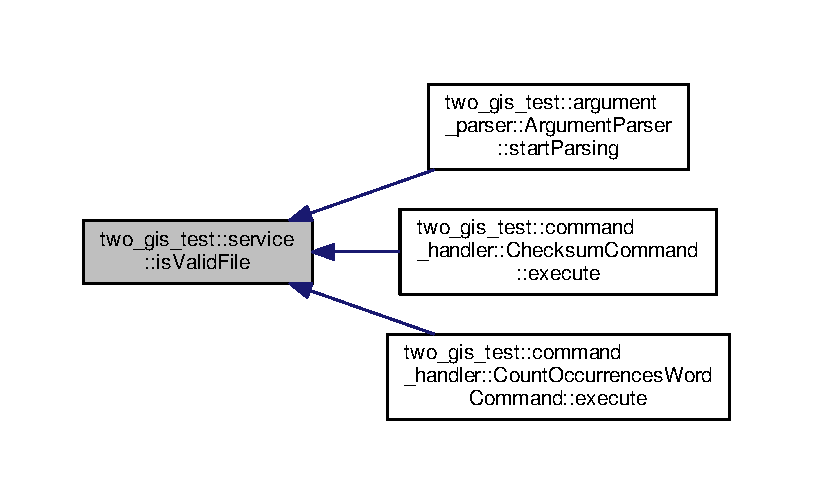
\includegraphics[width=350pt]{namespacetwo__gis__test_1_1service_ae373eed74cdbd1fd23749a7cd25ec61f_icgraph}
\end{center}
\end{figure}



\chapter{Class Documentation}
\hypertarget{classtwo__gis__test_1_1argument__parser_1_1_args_parse_exception}{}\section{two\+\_\+gis\+\_\+test\+:\+:argument\+\_\+parser\+:\+:Args\+Parse\+Exception Class Reference}
\label{classtwo__gis__test_1_1argument__parser_1_1_args_parse_exception}\index{two\+\_\+gis\+\_\+test\+::argument\+\_\+parser\+::\+Args\+Parse\+Exception@{two\+\_\+gis\+\_\+test\+::argument\+\_\+parser\+::\+Args\+Parse\+Exception}}


{\ttfamily \#include $<$args\+\_\+parse\+\_\+exception.\+hpp$>$}



Inheritance diagram for two\+\_\+gis\+\_\+test\+:\+:argument\+\_\+parser\+:\+:Args\+Parse\+Exception\+:\nopagebreak
\begin{figure}[H]
\begin{center}
\leavevmode
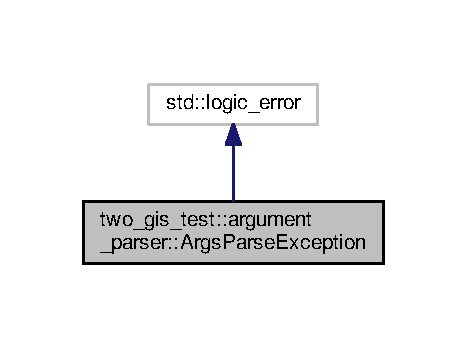
\includegraphics[width=224pt]{classtwo__gis__test_1_1argument__parser_1_1_args_parse_exception__inherit__graph}
\end{center}
\end{figure}


Collaboration diagram for two\+\_\+gis\+\_\+test\+:\+:argument\+\_\+parser\+:\+:Args\+Parse\+Exception\+:\nopagebreak
\begin{figure}[H]
\begin{center}
\leavevmode
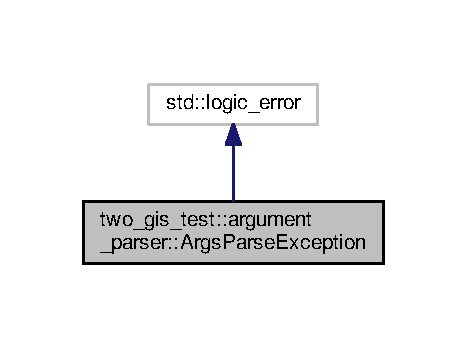
\includegraphics[width=224pt]{classtwo__gis__test_1_1argument__parser_1_1_args_parse_exception__coll__graph}
\end{center}
\end{figure}
\subsection*{Public Member Functions}
\begin{DoxyCompactItemize}
\item 
\hyperlink{classtwo__gis__test_1_1argument__parser_1_1_args_parse_exception_a768f3334c218c1f23729253926566325}{Args\+Parse\+Exception} (const std\+::string \&message)
\begin{DoxyCompactList}\small\item\em \hyperlink{classtwo__gis__test_1_1argument__parser_1_1_args_parse_exception}{Args\+Parse\+Exception} -\/ constructor. \end{DoxyCompactList}\item 
\hyperlink{classtwo__gis__test_1_1argument__parser_1_1_args_parse_exception_a6111f03bd59e8afe83de05c42aafebb2}{Args\+Parse\+Exception} (const char $\ast$message)
\begin{DoxyCompactList}\small\item\em \hyperlink{classtwo__gis__test_1_1argument__parser_1_1_args_parse_exception}{Args\+Parse\+Exception} -\/ constructor. \end{DoxyCompactList}\item 
\hyperlink{classtwo__gis__test_1_1argument__parser_1_1_args_parse_exception_ae9f418bfb4bf5ff1c5a4d8a0fe9a7ae5}{Args\+Parse\+Exception} (const \hyperlink{classtwo__gis__test_1_1argument__parser_1_1_args_parse_exception}{Args\+Parse\+Exception} \&)=default
\begin{DoxyCompactList}\small\item\em \hyperlink{classtwo__gis__test_1_1argument__parser_1_1_args_parse_exception}{Args\+Parse\+Exception} -\/ copy constructor. \end{DoxyCompactList}\item 
\hyperlink{classtwo__gis__test_1_1argument__parser_1_1_args_parse_exception}{Args\+Parse\+Exception} \& \hyperlink{classtwo__gis__test_1_1argument__parser_1_1_args_parse_exception_a93abbb3ad22dc77bc20dc9e09e7f3827}{operator=} (const \hyperlink{classtwo__gis__test_1_1argument__parser_1_1_args_parse_exception}{Args\+Parse\+Exception} \&)=default
\item 
\hyperlink{classtwo__gis__test_1_1argument__parser_1_1_args_parse_exception_a952e63dbd0b42100e44fa7a8b0572abb}{$\sim$\+Args\+Parse\+Exception} () override=default
\item 
const char $\ast$ \hyperlink{classtwo__gis__test_1_1argument__parser_1_1_args_parse_exception_a46924e2f070476eaf5091c2d19bdc57c}{what} () const override  throw ()
\begin{DoxyCompactList}\small\item\em what -\/ override method \end{DoxyCompactList}\end{DoxyCompactItemize}


\subsection{Detailed Description}
exception 

Definition at line 16 of file args\+\_\+parse\+\_\+exception.\+hpp.



\subsection{Constructor \& Destructor Documentation}
\index{two\+\_\+gis\+\_\+test\+::argument\+\_\+parser\+::\+Args\+Parse\+Exception@{two\+\_\+gis\+\_\+test\+::argument\+\_\+parser\+::\+Args\+Parse\+Exception}!Args\+Parse\+Exception@{Args\+Parse\+Exception}}
\index{Args\+Parse\+Exception@{Args\+Parse\+Exception}!two\+\_\+gis\+\_\+test\+::argument\+\_\+parser\+::\+Args\+Parse\+Exception@{two\+\_\+gis\+\_\+test\+::argument\+\_\+parser\+::\+Args\+Parse\+Exception}}
\subsubsection[{\texorpdfstring{Args\+Parse\+Exception(const std\+::string \&message)}{ArgsParseException(const std::string &message)}}]{\setlength{\rightskip}{0pt plus 5cm}two\+\_\+gis\+\_\+test\+::argument\+\_\+parser\+::\+Args\+Parse\+Exception\+::\+Args\+Parse\+Exception (
\begin{DoxyParamCaption}
\item[{const std\+::string \&}]{message}
\end{DoxyParamCaption}
)\hspace{0.3cm}{\ttfamily [explicit]}}\hypertarget{classtwo__gis__test_1_1argument__parser_1_1_args_parse_exception_a768f3334c218c1f23729253926566325}{}\label{classtwo__gis__test_1_1argument__parser_1_1_args_parse_exception_a768f3334c218c1f23729253926566325}


\hyperlink{classtwo__gis__test_1_1argument__parser_1_1_args_parse_exception}{Args\+Parse\+Exception} -\/ constructor. 


\begin{DoxyParams}{Parameters}
{\em message} & -\/ error message \\
\hline
\end{DoxyParams}


Definition at line 12 of file args\+\_\+parse\+\_\+exception.\+cpp.

\index{two\+\_\+gis\+\_\+test\+::argument\+\_\+parser\+::\+Args\+Parse\+Exception@{two\+\_\+gis\+\_\+test\+::argument\+\_\+parser\+::\+Args\+Parse\+Exception}!Args\+Parse\+Exception@{Args\+Parse\+Exception}}
\index{Args\+Parse\+Exception@{Args\+Parse\+Exception}!two\+\_\+gis\+\_\+test\+::argument\+\_\+parser\+::\+Args\+Parse\+Exception@{two\+\_\+gis\+\_\+test\+::argument\+\_\+parser\+::\+Args\+Parse\+Exception}}
\subsubsection[{\texorpdfstring{Args\+Parse\+Exception(const char $\ast$message)}{ArgsParseException(const char *message)}}]{\setlength{\rightskip}{0pt plus 5cm}two\+\_\+gis\+\_\+test\+::argument\+\_\+parser\+::\+Args\+Parse\+Exception\+::\+Args\+Parse\+Exception (
\begin{DoxyParamCaption}
\item[{const char $\ast$}]{message}
\end{DoxyParamCaption}
)\hspace{0.3cm}{\ttfamily [explicit]}}\hypertarget{classtwo__gis__test_1_1argument__parser_1_1_args_parse_exception_a6111f03bd59e8afe83de05c42aafebb2}{}\label{classtwo__gis__test_1_1argument__parser_1_1_args_parse_exception_a6111f03bd59e8afe83de05c42aafebb2}


\hyperlink{classtwo__gis__test_1_1argument__parser_1_1_args_parse_exception}{Args\+Parse\+Exception} -\/ constructor. 


\begin{DoxyParams}{Parameters}
{\em message} & \\
\hline
\end{DoxyParams}


Definition at line 19 of file args\+\_\+parse\+\_\+exception.\+cpp.

\index{two\+\_\+gis\+\_\+test\+::argument\+\_\+parser\+::\+Args\+Parse\+Exception@{two\+\_\+gis\+\_\+test\+::argument\+\_\+parser\+::\+Args\+Parse\+Exception}!Args\+Parse\+Exception@{Args\+Parse\+Exception}}
\index{Args\+Parse\+Exception@{Args\+Parse\+Exception}!two\+\_\+gis\+\_\+test\+::argument\+\_\+parser\+::\+Args\+Parse\+Exception@{two\+\_\+gis\+\_\+test\+::argument\+\_\+parser\+::\+Args\+Parse\+Exception}}
\subsubsection[{\texorpdfstring{Args\+Parse\+Exception(const Args\+Parse\+Exception \&)=default}{ArgsParseException(const ArgsParseException &)=default}}]{\setlength{\rightskip}{0pt plus 5cm}two\+\_\+gis\+\_\+test\+::argument\+\_\+parser\+::\+Args\+Parse\+Exception\+::\+Args\+Parse\+Exception (
\begin{DoxyParamCaption}
\item[{const {\bf Args\+Parse\+Exception} \&}]{}
\end{DoxyParamCaption}
)\hspace{0.3cm}{\ttfamily [default]}}\hypertarget{classtwo__gis__test_1_1argument__parser_1_1_args_parse_exception_ae9f418bfb4bf5ff1c5a4d8a0fe9a7ae5}{}\label{classtwo__gis__test_1_1argument__parser_1_1_args_parse_exception_ae9f418bfb4bf5ff1c5a4d8a0fe9a7ae5}


\hyperlink{classtwo__gis__test_1_1argument__parser_1_1_args_parse_exception}{Args\+Parse\+Exception} -\/ copy constructor. 

\index{two\+\_\+gis\+\_\+test\+::argument\+\_\+parser\+::\+Args\+Parse\+Exception@{two\+\_\+gis\+\_\+test\+::argument\+\_\+parser\+::\+Args\+Parse\+Exception}!````~Args\+Parse\+Exception@{$\sim$\+Args\+Parse\+Exception}}
\index{````~Args\+Parse\+Exception@{$\sim$\+Args\+Parse\+Exception}!two\+\_\+gis\+\_\+test\+::argument\+\_\+parser\+::\+Args\+Parse\+Exception@{two\+\_\+gis\+\_\+test\+::argument\+\_\+parser\+::\+Args\+Parse\+Exception}}
\subsubsection[{\texorpdfstring{$\sim$\+Args\+Parse\+Exception() override=default}{~ArgsParseException() override=default}}]{\setlength{\rightskip}{0pt plus 5cm}two\+\_\+gis\+\_\+test\+::argument\+\_\+parser\+::\+Args\+Parse\+Exception\+::$\sim$\+Args\+Parse\+Exception (
\begin{DoxyParamCaption}
{}
\end{DoxyParamCaption}
)\hspace{0.3cm}{\ttfamily [override]}, {\ttfamily [default]}}\hypertarget{classtwo__gis__test_1_1argument__parser_1_1_args_parse_exception_a952e63dbd0b42100e44fa7a8b0572abb}{}\label{classtwo__gis__test_1_1argument__parser_1_1_args_parse_exception_a952e63dbd0b42100e44fa7a8b0572abb}


\subsection{Member Function Documentation}
\index{two\+\_\+gis\+\_\+test\+::argument\+\_\+parser\+::\+Args\+Parse\+Exception@{two\+\_\+gis\+\_\+test\+::argument\+\_\+parser\+::\+Args\+Parse\+Exception}!operator=@{operator=}}
\index{operator=@{operator=}!two\+\_\+gis\+\_\+test\+::argument\+\_\+parser\+::\+Args\+Parse\+Exception@{two\+\_\+gis\+\_\+test\+::argument\+\_\+parser\+::\+Args\+Parse\+Exception}}
\subsubsection[{\texorpdfstring{operator=(const Args\+Parse\+Exception \&)=default}{operator=(const ArgsParseException &)=default}}]{\setlength{\rightskip}{0pt plus 5cm}{\bf Args\+Parse\+Exception}\& two\+\_\+gis\+\_\+test\+::argument\+\_\+parser\+::\+Args\+Parse\+Exception\+::operator= (
\begin{DoxyParamCaption}
\item[{const {\bf Args\+Parse\+Exception} \&}]{}
\end{DoxyParamCaption}
)\hspace{0.3cm}{\ttfamily [default]}}\hypertarget{classtwo__gis__test_1_1argument__parser_1_1_args_parse_exception_a93abbb3ad22dc77bc20dc9e09e7f3827}{}\label{classtwo__gis__test_1_1argument__parser_1_1_args_parse_exception_a93abbb3ad22dc77bc20dc9e09e7f3827}
\index{two\+\_\+gis\+\_\+test\+::argument\+\_\+parser\+::\+Args\+Parse\+Exception@{two\+\_\+gis\+\_\+test\+::argument\+\_\+parser\+::\+Args\+Parse\+Exception}!what@{what}}
\index{what@{what}!two\+\_\+gis\+\_\+test\+::argument\+\_\+parser\+::\+Args\+Parse\+Exception@{two\+\_\+gis\+\_\+test\+::argument\+\_\+parser\+::\+Args\+Parse\+Exception}}
\subsubsection[{\texorpdfstring{what() const override}{what() const override}}]{\setlength{\rightskip}{0pt plus 5cm}const char $\ast$ two\+\_\+gis\+\_\+test\+::argument\+\_\+parser\+::\+Args\+Parse\+Exception\+::what (
\begin{DoxyParamCaption}
{}
\end{DoxyParamCaption}
) const throw  ) \hspace{0.3cm}{\ttfamily [override]}}\hypertarget{classtwo__gis__test_1_1argument__parser_1_1_args_parse_exception_a46924e2f070476eaf5091c2d19bdc57c}{}\label{classtwo__gis__test_1_1argument__parser_1_1_args_parse_exception_a46924e2f070476eaf5091c2d19bdc57c}


what -\/ override method 

\begin{DoxyReturn}{Returns}
Returns a C-\/style character string describing the general cause of the current error (the same string passed to the ctor). 
\end{DoxyReturn}


Definition at line 15 of file args\+\_\+parse\+\_\+exception.\+cpp.



Here is the caller graph for this function\+:\nopagebreak
\begin{figure}[H]
\begin{center}
\leavevmode
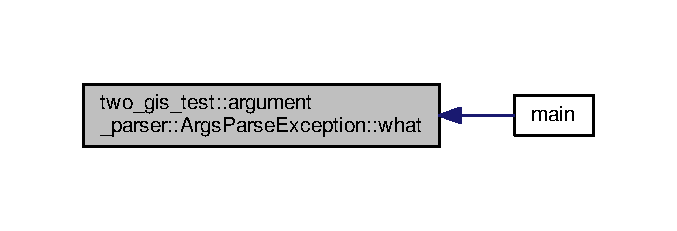
\includegraphics[width=325pt]{classtwo__gis__test_1_1argument__parser_1_1_args_parse_exception_a46924e2f070476eaf5091c2d19bdc57c_icgraph}
\end{center}
\end{figure}




The documentation for this class was generated from the following files\+:\begin{DoxyCompactItemize}
\item 
/home/boa/\+C\+Lion\+Projects/word\+\_\+counter/args\+\_\+parser/include/\hyperlink{args__parse__exception_8hpp}{args\+\_\+parse\+\_\+exception.\+hpp}\item 
/home/boa/\+C\+Lion\+Projects/word\+\_\+counter/args\+\_\+parser/src/\hyperlink{args__parse__exception_8cpp}{args\+\_\+parse\+\_\+exception.\+cpp}\end{DoxyCompactItemize}

\hypertarget{classtwo__gis__test_1_1argument__parser_1_1_argument_parser}{}\section{two\+\_\+gis\+\_\+test\+:\+:argument\+\_\+parser\+:\+:Argument\+Parser Class Reference}
\label{classtwo__gis__test_1_1argument__parser_1_1_argument_parser}\index{two\+\_\+gis\+\_\+test\+::argument\+\_\+parser\+::\+Argument\+Parser@{two\+\_\+gis\+\_\+test\+::argument\+\_\+parser\+::\+Argument\+Parser}}


{\ttfamily \#include $<$argument\+\_\+parser.\+hpp$>$}

\subsection*{Public Member Functions}
\begin{DoxyCompactItemize}
\item 
\hyperlink{classtwo__gis__test_1_1argument__parser_1_1_argument_parser_a60b6545a121f02ce271e98b40d7635fc}{Argument\+Parser} ()
\begin{DoxyCompactList}\small\item\em \hyperlink{classtwo__gis__test_1_1argument__parser_1_1_argument_parser}{Argument\+Parser} -\/ default constructor, init general\+Description\+\_\+. \end{DoxyCompactList}\item 
void \hyperlink{classtwo__gis__test_1_1argument__parser_1_1_argument_parser_a02248a1453c8dc2e947f173f9b5cfc9b}{start\+Parsing} (int argc, char $\ast$argv\mbox{[}$\,$\mbox{]})
\begin{DoxyCompactList}\small\item\em start\+Parsing start command line arguments parser \end{DoxyCompactList}\end{DoxyCompactItemize}
\subsection*{Public Attributes}
\begin{DoxyCompactItemize}
\item 
boost\+::signals2\+::signal$<$ void(std\+::string \&filename, std\+::string \&word)$>$ \hyperlink{classtwo__gis__test_1_1argument__parser_1_1_argument_parser_a9fdaea74b7ce00d7cc39c797745b9436}{count\+Occurrences\+Word}
\begin{DoxyCompactList}\small\item\em count -\/ program switching signal to word count mode \end{DoxyCompactList}\item 
boost\+::signals2\+::signal$<$ void(std\+::string \&filename)$>$ \hyperlink{classtwo__gis__test_1_1argument__parser_1_1_argument_parser_ac02b2454df0eb6f127cadb0ccfdad67c}{calculate\+Checksum}
\begin{DoxyCompactList}\small\item\em checksum -\/ the program switching signal to the Checksum calculation mode \end{DoxyCompactList}\end{DoxyCompactItemize}


\subsection{Detailed Description}


Definition at line 22 of file argument\+\_\+parser.\+hpp.



\subsection{Constructor \& Destructor Documentation}
\index{two\+\_\+gis\+\_\+test\+::argument\+\_\+parser\+::\+Argument\+Parser@{two\+\_\+gis\+\_\+test\+::argument\+\_\+parser\+::\+Argument\+Parser}!Argument\+Parser@{Argument\+Parser}}
\index{Argument\+Parser@{Argument\+Parser}!two\+\_\+gis\+\_\+test\+::argument\+\_\+parser\+::\+Argument\+Parser@{two\+\_\+gis\+\_\+test\+::argument\+\_\+parser\+::\+Argument\+Parser}}
\subsubsection[{\texorpdfstring{Argument\+Parser()}{ArgumentParser()}}]{\setlength{\rightskip}{0pt plus 5cm}two\+\_\+gis\+\_\+test\+::argument\+\_\+parser\+::\+Argument\+Parser\+::\+Argument\+Parser (
\begin{DoxyParamCaption}
{}
\end{DoxyParamCaption}
)}\hypertarget{classtwo__gis__test_1_1argument__parser_1_1_argument_parser_a60b6545a121f02ce271e98b40d7635fc}{}\label{classtwo__gis__test_1_1argument__parser_1_1_argument_parser_a60b6545a121f02ce271e98b40d7635fc}


\hyperlink{classtwo__gis__test_1_1argument__parser_1_1_argument_parser}{Argument\+Parser} -\/ default constructor, init general\+Description\+\_\+. 



Definition at line 9 of file argument\+\_\+parser.\+cpp.



\subsection{Member Function Documentation}
\index{two\+\_\+gis\+\_\+test\+::argument\+\_\+parser\+::\+Argument\+Parser@{two\+\_\+gis\+\_\+test\+::argument\+\_\+parser\+::\+Argument\+Parser}!start\+Parsing@{start\+Parsing}}
\index{start\+Parsing@{start\+Parsing}!two\+\_\+gis\+\_\+test\+::argument\+\_\+parser\+::\+Argument\+Parser@{two\+\_\+gis\+\_\+test\+::argument\+\_\+parser\+::\+Argument\+Parser}}
\subsubsection[{\texorpdfstring{start\+Parsing(int argc, char $\ast$argv[])}{startParsing(int argc, char *argv[])}}]{\setlength{\rightskip}{0pt plus 5cm}void two\+\_\+gis\+\_\+test\+::argument\+\_\+parser\+::\+Argument\+Parser\+::start\+Parsing (
\begin{DoxyParamCaption}
\item[{int}]{argc, }
\item[{char $\ast$}]{argv\mbox{[}$\,$\mbox{]}}
\end{DoxyParamCaption}
)}\hypertarget{classtwo__gis__test_1_1argument__parser_1_1_argument_parser_a02248a1453c8dc2e947f173f9b5cfc9b}{}\label{classtwo__gis__test_1_1argument__parser_1_1_argument_parser_a02248a1453c8dc2e947f173f9b5cfc9b}


start\+Parsing start command line arguments parser 


\begin{DoxyParams}{Parameters}
{\em argc} & count of arguments \\
\hline
{\em argv} & -\/ values of arguments \\
\hline
\end{DoxyParams}


Definition at line 36 of file argument\+\_\+parser.\+cpp.



Here is the call graph for this function\+:\nopagebreak
\begin{figure}[H]
\begin{center}
\leavevmode
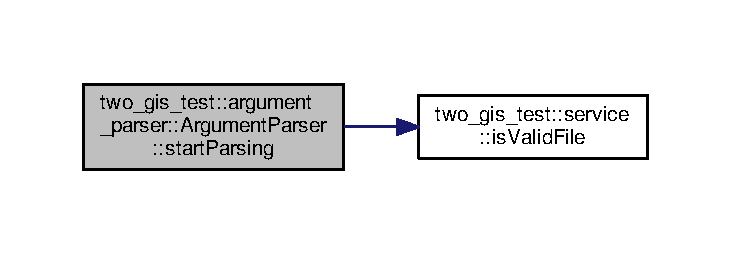
\includegraphics[width=350pt]{classtwo__gis__test_1_1argument__parser_1_1_argument_parser_a02248a1453c8dc2e947f173f9b5cfc9b_cgraph}
\end{center}
\end{figure}




\subsection{Member Data Documentation}
\index{two\+\_\+gis\+\_\+test\+::argument\+\_\+parser\+::\+Argument\+Parser@{two\+\_\+gis\+\_\+test\+::argument\+\_\+parser\+::\+Argument\+Parser}!calculate\+Checksum@{calculate\+Checksum}}
\index{calculate\+Checksum@{calculate\+Checksum}!two\+\_\+gis\+\_\+test\+::argument\+\_\+parser\+::\+Argument\+Parser@{two\+\_\+gis\+\_\+test\+::argument\+\_\+parser\+::\+Argument\+Parser}}
\subsubsection[{\texorpdfstring{calculate\+Checksum}{calculateChecksum}}]{\setlength{\rightskip}{0pt plus 5cm}boost\+::signals2\+::signal$<$void(std\+::string \&filename)$>$ two\+\_\+gis\+\_\+test\+::argument\+\_\+parser\+::\+Argument\+Parser\+::calculate\+Checksum}\hypertarget{classtwo__gis__test_1_1argument__parser_1_1_argument_parser_ac02b2454df0eb6f127cadb0ccfdad67c}{}\label{classtwo__gis__test_1_1argument__parser_1_1_argument_parser_ac02b2454df0eb6f127cadb0ccfdad67c}


checksum -\/ the program switching signal to the Checksum calculation mode 


\begin{DoxyParams}{Parameters}
{\em filename} & -\/ input file \\
\hline
\end{DoxyParams}


Definition at line 39 of file argument\+\_\+parser.\+hpp.

\index{two\+\_\+gis\+\_\+test\+::argument\+\_\+parser\+::\+Argument\+Parser@{two\+\_\+gis\+\_\+test\+::argument\+\_\+parser\+::\+Argument\+Parser}!count\+Occurrences\+Word@{count\+Occurrences\+Word}}
\index{count\+Occurrences\+Word@{count\+Occurrences\+Word}!two\+\_\+gis\+\_\+test\+::argument\+\_\+parser\+::\+Argument\+Parser@{two\+\_\+gis\+\_\+test\+::argument\+\_\+parser\+::\+Argument\+Parser}}
\subsubsection[{\texorpdfstring{count\+Occurrences\+Word}{countOccurrencesWord}}]{\setlength{\rightskip}{0pt plus 5cm}boost\+::signals2\+::signal$<$void(std\+::string \&filename, std\+::string \&word)$>$ two\+\_\+gis\+\_\+test\+::argument\+\_\+parser\+::\+Argument\+Parser\+::count\+Occurrences\+Word}\hypertarget{classtwo__gis__test_1_1argument__parser_1_1_argument_parser_a9fdaea74b7ce00d7cc39c797745b9436}{}\label{classtwo__gis__test_1_1argument__parser_1_1_argument_parser_a9fdaea74b7ce00d7cc39c797745b9436}


count -\/ program switching signal to word count mode 


\begin{DoxyParams}{Parameters}
{\em filename} & -\/ input file \\
\hline
{\em word} & -\/ search word \\
\hline
\end{DoxyParams}


Definition at line 33 of file argument\+\_\+parser.\+hpp.



The documentation for this class was generated from the following files\+:\begin{DoxyCompactItemize}
\item 
/home/boa/\+C\+Lion\+Projects/word\+\_\+counter/args\+\_\+parser/include/\hyperlink{argument__parser_8hpp}{argument\+\_\+parser.\+hpp}\item 
/home/boa/\+C\+Lion\+Projects/word\+\_\+counter/args\+\_\+parser/src/\hyperlink{argument__parser_8cpp}{argument\+\_\+parser.\+cpp}\end{DoxyCompactItemize}

\hypertarget{classtwo__gis__test_1_1command__handler_1_1_checksum_command}{}\section{two\+\_\+gis\+\_\+test\+:\+:command\+\_\+handler\+:\+:Checksum\+Command Class Reference}
\label{classtwo__gis__test_1_1command__handler_1_1_checksum_command}\index{two\+\_\+gis\+\_\+test\+::command\+\_\+handler\+::\+Checksum\+Command@{two\+\_\+gis\+\_\+test\+::command\+\_\+handler\+::\+Checksum\+Command}}


{\ttfamily \#include $<$checksum\+\_\+command.\+hpp$>$}



Inheritance diagram for two\+\_\+gis\+\_\+test\+:\+:command\+\_\+handler\+:\+:Checksum\+Command\+:\nopagebreak
\begin{figure}[H]
\begin{center}
\leavevmode
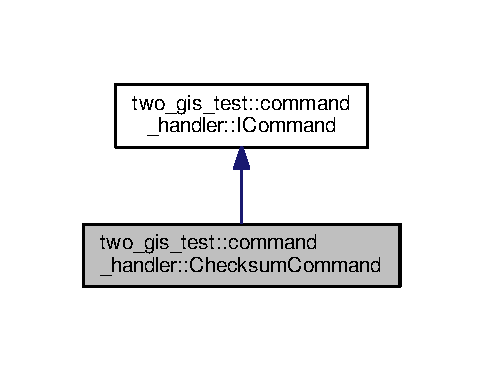
\includegraphics[width=232pt]{classtwo__gis__test_1_1command__handler_1_1_checksum_command__inherit__graph}
\end{center}
\end{figure}


Collaboration diagram for two\+\_\+gis\+\_\+test\+:\+:command\+\_\+handler\+:\+:Checksum\+Command\+:\nopagebreak
\begin{figure}[H]
\begin{center}
\leavevmode
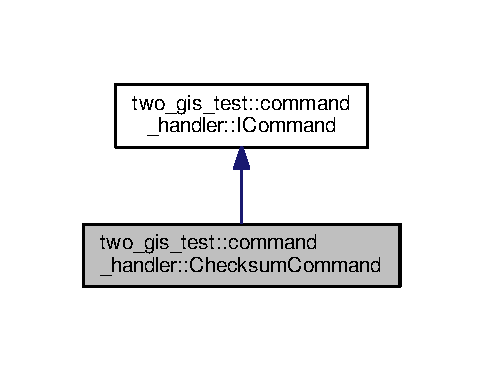
\includegraphics[width=232pt]{classtwo__gis__test_1_1command__handler_1_1_checksum_command__coll__graph}
\end{center}
\end{figure}
\subsection*{Public Member Functions}
\begin{DoxyCompactItemize}
\item 
\hyperlink{classtwo__gis__test_1_1command__handler_1_1_checksum_command_acd066f41f0b20846b6e593026695bdf5}{Checksum\+Command} (std\+::string \&filename)
\begin{DoxyCompactList}\small\item\em \hyperlink{classtwo__gis__test_1_1command__handler_1_1_checksum_command}{Checksum\+Command} -\/ constructor. \end{DoxyCompactList}\item 
\hyperlink{classtwo__gis__test_1_1command__handler_1_1_checksum_command_aba52fa430b7d227712e5edec74c78c20}{$\sim$\+Checksum\+Command} () override=default
\begin{DoxyCompactList}\small\item\em $\sim$\+Checksum\+Command -\/ destructor \end{DoxyCompactList}\item 
\hyperlink{classtwo__gis__test_1_1command__handler_1_1_checksum_command_a4be9b91a048631fdd97bcf28f2948cda}{Checksum\+Command} (const \hyperlink{classtwo__gis__test_1_1command__handler_1_1_checksum_command}{Checksum\+Command} \&)=default
\begin{DoxyCompactList}\small\item\em 
\begin{DoxyItemize}
\item \hyperlink{classtwo__gis__test_1_1command__handler_1_1_checksum_command}{Checksum\+Command} -\/ copy constructor 
\end{DoxyItemize}\end{DoxyCompactList}\item 
\hyperlink{classtwo__gis__test_1_1command__handler_1_1_checksum_command_a67da47fcd7e8d659ef8e030e5cd5fb2f}{Checksum\+Command} (\hyperlink{classtwo__gis__test_1_1command__handler_1_1_checksum_command}{Checksum\+Command} \&\&)=default
\begin{DoxyCompactList}\small\item\em \hyperlink{classtwo__gis__test_1_1command__handler_1_1_checksum_command}{Checksum\+Command} -\/ move constructor. \end{DoxyCompactList}\item 
\hyperlink{classtwo__gis__test_1_1command__handler_1_1_checksum_command}{Checksum\+Command} \& \hyperlink{classtwo__gis__test_1_1command__handler_1_1_checksum_command_a7603c6b9136cba7074cac4deb37e44ef}{operator=} (const \hyperlink{classtwo__gis__test_1_1command__handler_1_1_checksum_command}{Checksum\+Command} \&)=default
\begin{DoxyCompactList}\small\item\em operator= copy assignment operator \end{DoxyCompactList}\item 
\hyperlink{classtwo__gis__test_1_1command__handler_1_1_checksum_command}{Checksum\+Command} \& \hyperlink{classtwo__gis__test_1_1command__handler_1_1_checksum_command_a3095709e84c5cd873a181608cf543cc3}{operator=} (\hyperlink{classtwo__gis__test_1_1command__handler_1_1_checksum_command}{Checksum\+Command} \&\&)=default
\begin{DoxyCompactList}\small\item\em operator= move assignment operator \end{DoxyCompactList}\item 
void \hyperlink{classtwo__gis__test_1_1command__handler_1_1_checksum_command_a3ab082ac86155aa117e9870011a791f2}{execute} () override
\begin{DoxyCompactList}\small\item\em execute -\/ override method, calculate checksum \end{DoxyCompactList}\end{DoxyCompactItemize}


\subsection{Detailed Description}
\hyperlink{classtwo__gis__test_1_1command__handler_1_1_i_command}{I\+Command} interface 

Definition at line 17 of file checksum\+\_\+command.\+hpp.



\subsection{Constructor \& Destructor Documentation}
\index{two\+\_\+gis\+\_\+test\+::command\+\_\+handler\+::\+Checksum\+Command@{two\+\_\+gis\+\_\+test\+::command\+\_\+handler\+::\+Checksum\+Command}!Checksum\+Command@{Checksum\+Command}}
\index{Checksum\+Command@{Checksum\+Command}!two\+\_\+gis\+\_\+test\+::command\+\_\+handler\+::\+Checksum\+Command@{two\+\_\+gis\+\_\+test\+::command\+\_\+handler\+::\+Checksum\+Command}}
\subsubsection[{\texorpdfstring{Checksum\+Command(std\+::string \&filename)}{ChecksumCommand(std::string &filename)}}]{\setlength{\rightskip}{0pt plus 5cm}two\+\_\+gis\+\_\+test\+::command\+\_\+handler\+::\+Checksum\+Command\+::\+Checksum\+Command (
\begin{DoxyParamCaption}
\item[{std\+::string \&}]{filename}
\end{DoxyParamCaption}
)\hspace{0.3cm}{\ttfamily [explicit]}}\hypertarget{classtwo__gis__test_1_1command__handler_1_1_checksum_command_acd066f41f0b20846b6e593026695bdf5}{}\label{classtwo__gis__test_1_1command__handler_1_1_checksum_command_acd066f41f0b20846b6e593026695bdf5}


\hyperlink{classtwo__gis__test_1_1command__handler_1_1_checksum_command}{Checksum\+Command} -\/ constructor. 


\begin{DoxyParams}{Parameters}
{\em filename} & -\/ input file \\
\hline
\end{DoxyParams}


Definition at line 16 of file checksum\+\_\+command.\+cpp.

\index{two\+\_\+gis\+\_\+test\+::command\+\_\+handler\+::\+Checksum\+Command@{two\+\_\+gis\+\_\+test\+::command\+\_\+handler\+::\+Checksum\+Command}!````~Checksum\+Command@{$\sim$\+Checksum\+Command}}
\index{````~Checksum\+Command@{$\sim$\+Checksum\+Command}!two\+\_\+gis\+\_\+test\+::command\+\_\+handler\+::\+Checksum\+Command@{two\+\_\+gis\+\_\+test\+::command\+\_\+handler\+::\+Checksum\+Command}}
\subsubsection[{\texorpdfstring{$\sim$\+Checksum\+Command() override=default}{~ChecksumCommand() override=default}}]{\setlength{\rightskip}{0pt plus 5cm}two\+\_\+gis\+\_\+test\+::command\+\_\+handler\+::\+Checksum\+Command\+::$\sim$\+Checksum\+Command (
\begin{DoxyParamCaption}
{}
\end{DoxyParamCaption}
)\hspace{0.3cm}{\ttfamily [override]}, {\ttfamily [default]}}\hypertarget{classtwo__gis__test_1_1command__handler_1_1_checksum_command_aba52fa430b7d227712e5edec74c78c20}{}\label{classtwo__gis__test_1_1command__handler_1_1_checksum_command_aba52fa430b7d227712e5edec74c78c20}


$\sim$\+Checksum\+Command -\/ destructor 

\index{two\+\_\+gis\+\_\+test\+::command\+\_\+handler\+::\+Checksum\+Command@{two\+\_\+gis\+\_\+test\+::command\+\_\+handler\+::\+Checksum\+Command}!Checksum\+Command@{Checksum\+Command}}
\index{Checksum\+Command@{Checksum\+Command}!two\+\_\+gis\+\_\+test\+::command\+\_\+handler\+::\+Checksum\+Command@{two\+\_\+gis\+\_\+test\+::command\+\_\+handler\+::\+Checksum\+Command}}
\subsubsection[{\texorpdfstring{Checksum\+Command(const Checksum\+Command \&)=default}{ChecksumCommand(const ChecksumCommand &)=default}}]{\setlength{\rightskip}{0pt plus 5cm}two\+\_\+gis\+\_\+test\+::command\+\_\+handler\+::\+Checksum\+Command\+::\+Checksum\+Command (
\begin{DoxyParamCaption}
\item[{const {\bf Checksum\+Command} \&}]{}
\end{DoxyParamCaption}
)\hspace{0.3cm}{\ttfamily [default]}}\hypertarget{classtwo__gis__test_1_1command__handler_1_1_checksum_command_a4be9b91a048631fdd97bcf28f2948cda}{}\label{classtwo__gis__test_1_1command__handler_1_1_checksum_command_a4be9b91a048631fdd97bcf28f2948cda}



\begin{DoxyItemize}
\item \hyperlink{classtwo__gis__test_1_1command__handler_1_1_checksum_command}{Checksum\+Command} -\/ copy constructor 
\end{DoxyItemize}

\index{two\+\_\+gis\+\_\+test\+::command\+\_\+handler\+::\+Checksum\+Command@{two\+\_\+gis\+\_\+test\+::command\+\_\+handler\+::\+Checksum\+Command}!Checksum\+Command@{Checksum\+Command}}
\index{Checksum\+Command@{Checksum\+Command}!two\+\_\+gis\+\_\+test\+::command\+\_\+handler\+::\+Checksum\+Command@{two\+\_\+gis\+\_\+test\+::command\+\_\+handler\+::\+Checksum\+Command}}
\subsubsection[{\texorpdfstring{Checksum\+Command(\+Checksum\+Command \&\&)=default}{ChecksumCommand(ChecksumCommand &&)=default}}]{\setlength{\rightskip}{0pt plus 5cm}two\+\_\+gis\+\_\+test\+::command\+\_\+handler\+::\+Checksum\+Command\+::\+Checksum\+Command (
\begin{DoxyParamCaption}
\item[{{\bf Checksum\+Command} \&\&}]{}
\end{DoxyParamCaption}
)\hspace{0.3cm}{\ttfamily [default]}}\hypertarget{classtwo__gis__test_1_1command__handler_1_1_checksum_command_a67da47fcd7e8d659ef8e030e5cd5fb2f}{}\label{classtwo__gis__test_1_1command__handler_1_1_checksum_command_a67da47fcd7e8d659ef8e030e5cd5fb2f}


\hyperlink{classtwo__gis__test_1_1command__handler_1_1_checksum_command}{Checksum\+Command} -\/ move constructor. 



\subsection{Member Function Documentation}
\index{two\+\_\+gis\+\_\+test\+::command\+\_\+handler\+::\+Checksum\+Command@{two\+\_\+gis\+\_\+test\+::command\+\_\+handler\+::\+Checksum\+Command}!execute@{execute}}
\index{execute@{execute}!two\+\_\+gis\+\_\+test\+::command\+\_\+handler\+::\+Checksum\+Command@{two\+\_\+gis\+\_\+test\+::command\+\_\+handler\+::\+Checksum\+Command}}
\subsubsection[{\texorpdfstring{execute() override}{execute() override}}]{\setlength{\rightskip}{0pt plus 5cm}void two\+\_\+gis\+\_\+test\+::command\+\_\+handler\+::\+Checksum\+Command\+::execute (
\begin{DoxyParamCaption}
{}
\end{DoxyParamCaption}
)\hspace{0.3cm}{\ttfamily [override]}, {\ttfamily [virtual]}}\hypertarget{classtwo__gis__test_1_1command__handler_1_1_checksum_command_a3ab082ac86155aa117e9870011a791f2}{}\label{classtwo__gis__test_1_1command__handler_1_1_checksum_command_a3ab082ac86155aa117e9870011a791f2}


execute -\/ override method, calculate checksum 



Implements \hyperlink{classtwo__gis__test_1_1command__handler_1_1_i_command_a3674f79550d1ca7923a0c84c8fe0258f}{two\+\_\+gis\+\_\+test\+::command\+\_\+handler\+::\+I\+Command}.



Definition at line 19 of file checksum\+\_\+command.\+cpp.



Here is the call graph for this function\+:\nopagebreak
\begin{figure}[H]
\begin{center}
\leavevmode
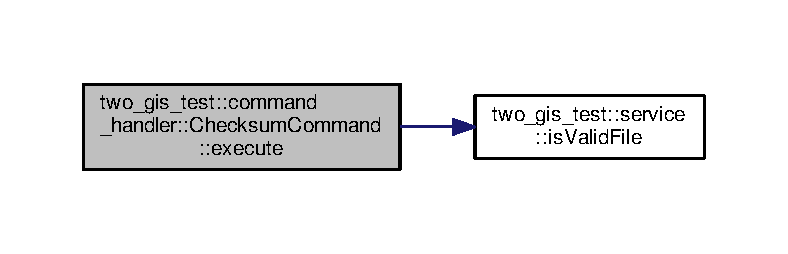
\includegraphics[width=350pt]{classtwo__gis__test_1_1command__handler_1_1_checksum_command_a3ab082ac86155aa117e9870011a791f2_cgraph}
\end{center}
\end{figure}


\index{two\+\_\+gis\+\_\+test\+::command\+\_\+handler\+::\+Checksum\+Command@{two\+\_\+gis\+\_\+test\+::command\+\_\+handler\+::\+Checksum\+Command}!operator=@{operator=}}
\index{operator=@{operator=}!two\+\_\+gis\+\_\+test\+::command\+\_\+handler\+::\+Checksum\+Command@{two\+\_\+gis\+\_\+test\+::command\+\_\+handler\+::\+Checksum\+Command}}
\subsubsection[{\texorpdfstring{operator=(const Checksum\+Command \&)=default}{operator=(const ChecksumCommand &)=default}}]{\setlength{\rightskip}{0pt plus 5cm}{\bf Checksum\+Command}\& two\+\_\+gis\+\_\+test\+::command\+\_\+handler\+::\+Checksum\+Command\+::operator= (
\begin{DoxyParamCaption}
\item[{const {\bf Checksum\+Command} \&}]{}
\end{DoxyParamCaption}
)\hspace{0.3cm}{\ttfamily [default]}}\hypertarget{classtwo__gis__test_1_1command__handler_1_1_checksum_command_a7603c6b9136cba7074cac4deb37e44ef}{}\label{classtwo__gis__test_1_1command__handler_1_1_checksum_command_a7603c6b9136cba7074cac4deb37e44ef}


operator= copy assignment operator 

\index{two\+\_\+gis\+\_\+test\+::command\+\_\+handler\+::\+Checksum\+Command@{two\+\_\+gis\+\_\+test\+::command\+\_\+handler\+::\+Checksum\+Command}!operator=@{operator=}}
\index{operator=@{operator=}!two\+\_\+gis\+\_\+test\+::command\+\_\+handler\+::\+Checksum\+Command@{two\+\_\+gis\+\_\+test\+::command\+\_\+handler\+::\+Checksum\+Command}}
\subsubsection[{\texorpdfstring{operator=(\+Checksum\+Command \&\&)=default}{operator=(ChecksumCommand &&)=default}}]{\setlength{\rightskip}{0pt plus 5cm}{\bf Checksum\+Command}\& two\+\_\+gis\+\_\+test\+::command\+\_\+handler\+::\+Checksum\+Command\+::operator= (
\begin{DoxyParamCaption}
\item[{{\bf Checksum\+Command} \&\&}]{}
\end{DoxyParamCaption}
)\hspace{0.3cm}{\ttfamily [default]}}\hypertarget{classtwo__gis__test_1_1command__handler_1_1_checksum_command_a3095709e84c5cd873a181608cf543cc3}{}\label{classtwo__gis__test_1_1command__handler_1_1_checksum_command_a3095709e84c5cd873a181608cf543cc3}


operator= move assignment operator 



The documentation for this class was generated from the following files\+:\begin{DoxyCompactItemize}
\item 
/home/boa/\+C\+Lion\+Projects/word\+\_\+counter/command\+\_\+handler/include/\hyperlink{checksum__command_8hpp}{checksum\+\_\+command.\+hpp}\item 
/home/boa/\+C\+Lion\+Projects/word\+\_\+counter/command\+\_\+handler/src/\hyperlink{checksum__command_8cpp}{checksum\+\_\+command.\+cpp}\end{DoxyCompactItemize}

\hypertarget{classtwo__gis__test_1_1command__handler_1_1_command_handler}{}\section{two\+\_\+gis\+\_\+test\+:\+:command\+\_\+handler\+:\+:Command\+Handler Class Reference}
\label{classtwo__gis__test_1_1command__handler_1_1_command_handler}\index{two\+\_\+gis\+\_\+test\+::command\+\_\+handler\+::\+Command\+Handler@{two\+\_\+gis\+\_\+test\+::command\+\_\+handler\+::\+Command\+Handler}}


{\ttfamily \#include $<$command\+\_\+handler.\+hpp$>$}

\subsection*{Public Member Functions}
\begin{DoxyCompactItemize}
\item 
\hyperlink{classtwo__gis__test_1_1command__handler_1_1_command_handler_ae9dd6f4dd96935fee159c1d896ff28a2}{Command\+Handler} ()=default
\begin{DoxyCompactList}\small\item\em \hyperlink{classtwo__gis__test_1_1command__handler_1_1_command_handler}{Command\+Handler} -\/ constructor. \end{DoxyCompactList}\item 
\hyperlink{classtwo__gis__test_1_1command__handler_1_1_command_handler_a845742e513ce6278dfd625629aa83d61}{$\sim$\+Command\+Handler} ()=default
\begin{DoxyCompactList}\small\item\em $\sim$\+Command\+Handler -\/ destructor \end{DoxyCompactList}\item 
\hyperlink{classtwo__gis__test_1_1command__handler_1_1_command_handler_a7e9058925ed115c7ef068a7e07cc1602}{Command\+Handler} (const \hyperlink{classtwo__gis__test_1_1command__handler_1_1_command_handler}{Command\+Handler} \&)=default
\begin{DoxyCompactList}\small\item\em \hyperlink{classtwo__gis__test_1_1command__handler_1_1_command_handler}{Command\+Handler} -\/ copy constructor. \end{DoxyCompactList}\item 
\hyperlink{classtwo__gis__test_1_1command__handler_1_1_command_handler_ae58ae9fd0d34f1ad2ee56fd454efc07d}{Command\+Handler} (\hyperlink{classtwo__gis__test_1_1command__handler_1_1_command_handler}{Command\+Handler} \&\&)=default
\begin{DoxyCompactList}\small\item\em 
\begin{DoxyItemize}
\item move constructor 
\end{DoxyItemize}\end{DoxyCompactList}\item 
\hyperlink{classtwo__gis__test_1_1command__handler_1_1_command_handler}{Command\+Handler} \& \hyperlink{classtwo__gis__test_1_1command__handler_1_1_command_handler_af1f40cd93f9c9d73356579f0cead177e}{operator=} (const \hyperlink{classtwo__gis__test_1_1command__handler_1_1_command_handler}{Command\+Handler} \&)=default
\begin{DoxyCompactList}\small\item\em operator= copy assignment operator \end{DoxyCompactList}\item 
\hyperlink{classtwo__gis__test_1_1command__handler_1_1_command_handler}{Command\+Handler} \& \hyperlink{classtwo__gis__test_1_1command__handler_1_1_command_handler_ac6132ef7dfcb0150b8cf12470f91a679}{operator=} (\hyperlink{classtwo__gis__test_1_1command__handler_1_1_command_handler}{Command\+Handler} \&\&)=default
\begin{DoxyCompactList}\small\item\em operator= move assignment operator \end{DoxyCompactList}\item 
void \hyperlink{classtwo__gis__test_1_1command__handler_1_1_command_handler_abbeae2ec331ce769bee29f324dde9f4a}{start} (std\+::shared\+\_\+ptr$<$ \hyperlink{classtwo__gis__test_1_1command__handler_1_1_i_command}{I\+Command} $>$ command)
\begin{DoxyCompactList}\small\item\em start -\/ run command execution of the command \end{DoxyCompactList}\end{DoxyCompactItemize}


\subsection{Detailed Description}
classical description (GoF) Receiver, executes commands 

Definition at line 20 of file command\+\_\+handler.\+hpp.



\subsection{Constructor \& Destructor Documentation}
\index{two\+\_\+gis\+\_\+test\+::command\+\_\+handler\+::\+Command\+Handler@{two\+\_\+gis\+\_\+test\+::command\+\_\+handler\+::\+Command\+Handler}!Command\+Handler@{Command\+Handler}}
\index{Command\+Handler@{Command\+Handler}!two\+\_\+gis\+\_\+test\+::command\+\_\+handler\+::\+Command\+Handler@{two\+\_\+gis\+\_\+test\+::command\+\_\+handler\+::\+Command\+Handler}}
\subsubsection[{\texorpdfstring{Command\+Handler()=default}{CommandHandler()=default}}]{\setlength{\rightskip}{0pt plus 5cm}two\+\_\+gis\+\_\+test\+::command\+\_\+handler\+::\+Command\+Handler\+::\+Command\+Handler (
\begin{DoxyParamCaption}
{}
\end{DoxyParamCaption}
)\hspace{0.3cm}{\ttfamily [default]}}\hypertarget{classtwo__gis__test_1_1command__handler_1_1_command_handler_ae9dd6f4dd96935fee159c1d896ff28a2}{}\label{classtwo__gis__test_1_1command__handler_1_1_command_handler_ae9dd6f4dd96935fee159c1d896ff28a2}


\hyperlink{classtwo__gis__test_1_1command__handler_1_1_command_handler}{Command\+Handler} -\/ constructor. 

\index{two\+\_\+gis\+\_\+test\+::command\+\_\+handler\+::\+Command\+Handler@{two\+\_\+gis\+\_\+test\+::command\+\_\+handler\+::\+Command\+Handler}!````~Command\+Handler@{$\sim$\+Command\+Handler}}
\index{````~Command\+Handler@{$\sim$\+Command\+Handler}!two\+\_\+gis\+\_\+test\+::command\+\_\+handler\+::\+Command\+Handler@{two\+\_\+gis\+\_\+test\+::command\+\_\+handler\+::\+Command\+Handler}}
\subsubsection[{\texorpdfstring{$\sim$\+Command\+Handler()=default}{~CommandHandler()=default}}]{\setlength{\rightskip}{0pt plus 5cm}two\+\_\+gis\+\_\+test\+::command\+\_\+handler\+::\+Command\+Handler\+::$\sim$\+Command\+Handler (
\begin{DoxyParamCaption}
{}
\end{DoxyParamCaption}
)\hspace{0.3cm}{\ttfamily [default]}}\hypertarget{classtwo__gis__test_1_1command__handler_1_1_command_handler_a845742e513ce6278dfd625629aa83d61}{}\label{classtwo__gis__test_1_1command__handler_1_1_command_handler_a845742e513ce6278dfd625629aa83d61}


$\sim$\+Command\+Handler -\/ destructor 

\index{two\+\_\+gis\+\_\+test\+::command\+\_\+handler\+::\+Command\+Handler@{two\+\_\+gis\+\_\+test\+::command\+\_\+handler\+::\+Command\+Handler}!Command\+Handler@{Command\+Handler}}
\index{Command\+Handler@{Command\+Handler}!two\+\_\+gis\+\_\+test\+::command\+\_\+handler\+::\+Command\+Handler@{two\+\_\+gis\+\_\+test\+::command\+\_\+handler\+::\+Command\+Handler}}
\subsubsection[{\texorpdfstring{Command\+Handler(const Command\+Handler \&)=default}{CommandHandler(const CommandHandler &)=default}}]{\setlength{\rightskip}{0pt plus 5cm}two\+\_\+gis\+\_\+test\+::command\+\_\+handler\+::\+Command\+Handler\+::\+Command\+Handler (
\begin{DoxyParamCaption}
\item[{const {\bf Command\+Handler} \&}]{}
\end{DoxyParamCaption}
)\hspace{0.3cm}{\ttfamily [default]}}\hypertarget{classtwo__gis__test_1_1command__handler_1_1_command_handler_a7e9058925ed115c7ef068a7e07cc1602}{}\label{classtwo__gis__test_1_1command__handler_1_1_command_handler_a7e9058925ed115c7ef068a7e07cc1602}


\hyperlink{classtwo__gis__test_1_1command__handler_1_1_command_handler}{Command\+Handler} -\/ copy constructor. 

\index{two\+\_\+gis\+\_\+test\+::command\+\_\+handler\+::\+Command\+Handler@{two\+\_\+gis\+\_\+test\+::command\+\_\+handler\+::\+Command\+Handler}!Command\+Handler@{Command\+Handler}}
\index{Command\+Handler@{Command\+Handler}!two\+\_\+gis\+\_\+test\+::command\+\_\+handler\+::\+Command\+Handler@{two\+\_\+gis\+\_\+test\+::command\+\_\+handler\+::\+Command\+Handler}}
\subsubsection[{\texorpdfstring{Command\+Handler(\+Command\+Handler \&\&)=default}{CommandHandler(CommandHandler &&)=default}}]{\setlength{\rightskip}{0pt plus 5cm}two\+\_\+gis\+\_\+test\+::command\+\_\+handler\+::\+Command\+Handler\+::\+Command\+Handler (
\begin{DoxyParamCaption}
\item[{{\bf Command\+Handler} \&\&}]{}
\end{DoxyParamCaption}
)\hspace{0.3cm}{\ttfamily [default]}}\hypertarget{classtwo__gis__test_1_1command__handler_1_1_command_handler_ae58ae9fd0d34f1ad2ee56fd454efc07d}{}\label{classtwo__gis__test_1_1command__handler_1_1_command_handler_ae58ae9fd0d34f1ad2ee56fd454efc07d}



\begin{DoxyItemize}
\item move constructor 
\end{DoxyItemize}



\subsection{Member Function Documentation}
\index{two\+\_\+gis\+\_\+test\+::command\+\_\+handler\+::\+Command\+Handler@{two\+\_\+gis\+\_\+test\+::command\+\_\+handler\+::\+Command\+Handler}!operator=@{operator=}}
\index{operator=@{operator=}!two\+\_\+gis\+\_\+test\+::command\+\_\+handler\+::\+Command\+Handler@{two\+\_\+gis\+\_\+test\+::command\+\_\+handler\+::\+Command\+Handler}}
\subsubsection[{\texorpdfstring{operator=(const Command\+Handler \&)=default}{operator=(const CommandHandler &)=default}}]{\setlength{\rightskip}{0pt plus 5cm}{\bf Command\+Handler}\& two\+\_\+gis\+\_\+test\+::command\+\_\+handler\+::\+Command\+Handler\+::operator= (
\begin{DoxyParamCaption}
\item[{const {\bf Command\+Handler} \&}]{}
\end{DoxyParamCaption}
)\hspace{0.3cm}{\ttfamily [default]}}\hypertarget{classtwo__gis__test_1_1command__handler_1_1_command_handler_af1f40cd93f9c9d73356579f0cead177e}{}\label{classtwo__gis__test_1_1command__handler_1_1_command_handler_af1f40cd93f9c9d73356579f0cead177e}


operator= copy assignment operator 

\index{two\+\_\+gis\+\_\+test\+::command\+\_\+handler\+::\+Command\+Handler@{two\+\_\+gis\+\_\+test\+::command\+\_\+handler\+::\+Command\+Handler}!operator=@{operator=}}
\index{operator=@{operator=}!two\+\_\+gis\+\_\+test\+::command\+\_\+handler\+::\+Command\+Handler@{two\+\_\+gis\+\_\+test\+::command\+\_\+handler\+::\+Command\+Handler}}
\subsubsection[{\texorpdfstring{operator=(\+Command\+Handler \&\&)=default}{operator=(CommandHandler &&)=default}}]{\setlength{\rightskip}{0pt plus 5cm}{\bf Command\+Handler}\& two\+\_\+gis\+\_\+test\+::command\+\_\+handler\+::\+Command\+Handler\+::operator= (
\begin{DoxyParamCaption}
\item[{{\bf Command\+Handler} \&\&}]{}
\end{DoxyParamCaption}
)\hspace{0.3cm}{\ttfamily [default]}}\hypertarget{classtwo__gis__test_1_1command__handler_1_1_command_handler_ac6132ef7dfcb0150b8cf12470f91a679}{}\label{classtwo__gis__test_1_1command__handler_1_1_command_handler_ac6132ef7dfcb0150b8cf12470f91a679}


operator= move assignment operator 

\index{two\+\_\+gis\+\_\+test\+::command\+\_\+handler\+::\+Command\+Handler@{two\+\_\+gis\+\_\+test\+::command\+\_\+handler\+::\+Command\+Handler}!start@{start}}
\index{start@{start}!two\+\_\+gis\+\_\+test\+::command\+\_\+handler\+::\+Command\+Handler@{two\+\_\+gis\+\_\+test\+::command\+\_\+handler\+::\+Command\+Handler}}
\subsubsection[{\texorpdfstring{start(std\+::shared\+\_\+ptr$<$ I\+Command $>$ command)}{start(std::shared_ptr< ICommand > command)}}]{\setlength{\rightskip}{0pt plus 5cm}void two\+\_\+gis\+\_\+test\+::command\+\_\+handler\+::\+Command\+Handler\+::start (
\begin{DoxyParamCaption}
\item[{std\+::shared\+\_\+ptr$<$ {\bf I\+Command} $>$}]{command}
\end{DoxyParamCaption}
)}\hypertarget{classtwo__gis__test_1_1command__handler_1_1_command_handler_abbeae2ec331ce769bee29f324dde9f4a}{}\label{classtwo__gis__test_1_1command__handler_1_1_command_handler_abbeae2ec331ce769bee29f324dde9f4a}


start -\/ run command execution of the command 


\begin{DoxyParams}{Parameters}
{\em command} & -\/ command to be executed \\
\hline
\end{DoxyParams}


Definition at line 9 of file command\+\_\+handler.\+cpp.



The documentation for this class was generated from the following files\+:\begin{DoxyCompactItemize}
\item 
/home/boa/\+C\+Lion\+Projects/word\+\_\+counter/command\+\_\+handler/include/\hyperlink{command__handler_8hpp}{command\+\_\+handler.\+hpp}\item 
/home/boa/\+C\+Lion\+Projects/word\+\_\+counter/command\+\_\+handler/src/\hyperlink{command__handler_8cpp}{command\+\_\+handler.\+cpp}\end{DoxyCompactItemize}

\hypertarget{classtwo__gis__test_1_1command__handler_1_1_count_occurrences_word_command}{}\section{two\+\_\+gis\+\_\+test\+:\+:command\+\_\+handler\+:\+:Count\+Occurrences\+Word\+Command Class Reference}
\label{classtwo__gis__test_1_1command__handler_1_1_count_occurrences_word_command}\index{two\+\_\+gis\+\_\+test\+::command\+\_\+handler\+::\+Count\+Occurrences\+Word\+Command@{two\+\_\+gis\+\_\+test\+::command\+\_\+handler\+::\+Count\+Occurrences\+Word\+Command}}


{\ttfamily \#include $<$count\+\_\+occurrences\+\_\+word\+\_\+command.\+hpp$>$}



Inheritance diagram for two\+\_\+gis\+\_\+test\+:\+:command\+\_\+handler\+:\+:Count\+Occurrences\+Word\+Command\+:\nopagebreak
\begin{figure}[H]
\begin{center}
\leavevmode
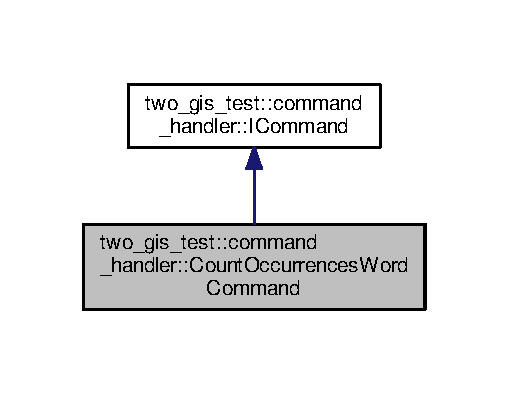
\includegraphics[width=244pt]{classtwo__gis__test_1_1command__handler_1_1_count_occurrences_word_command__inherit__graph}
\end{center}
\end{figure}


Collaboration diagram for two\+\_\+gis\+\_\+test\+:\+:command\+\_\+handler\+:\+:Count\+Occurrences\+Word\+Command\+:\nopagebreak
\begin{figure}[H]
\begin{center}
\leavevmode
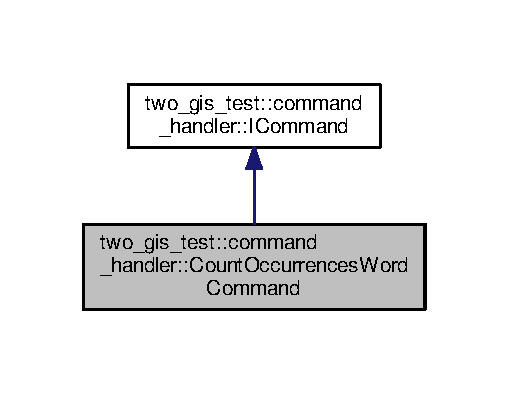
\includegraphics[width=244pt]{classtwo__gis__test_1_1command__handler_1_1_count_occurrences_word_command__coll__graph}
\end{center}
\end{figure}
\subsection*{Public Member Functions}
\begin{DoxyCompactItemize}
\item 
\hyperlink{classtwo__gis__test_1_1command__handler_1_1_count_occurrences_word_command_a08527c551b89b5dcaf41b05364bff426}{Count\+Occurrences\+Word\+Command} (std\+::string \&filename, std\+::string \&search\+Word)
\begin{DoxyCompactList}\small\item\em \hyperlink{classtwo__gis__test_1_1command__handler_1_1_count_occurrences_word_command}{Count\+Occurrences\+Word\+Command} -\/ constructor. \end{DoxyCompactList}\item 
\hyperlink{classtwo__gis__test_1_1command__handler_1_1_count_occurrences_word_command_a774bf6c5dc0ec6e458633e35cff74afa}{$\sim$\+Count\+Occurrences\+Word\+Command} () override=default
\begin{DoxyCompactList}\small\item\em $\sim$\+Count\+Occurrences\+Word\+Command -\/ destructor \end{DoxyCompactList}\item 
\hyperlink{classtwo__gis__test_1_1command__handler_1_1_count_occurrences_word_command_abf0daa24ed02f804727da6976559bf17}{Count\+Occurrences\+Word\+Command} (const \hyperlink{classtwo__gis__test_1_1command__handler_1_1_count_occurrences_word_command}{Count\+Occurrences\+Word\+Command} \&)=default
\begin{DoxyCompactList}\small\item\em \hyperlink{classtwo__gis__test_1_1command__handler_1_1_count_occurrences_word_command}{Count\+Occurrences\+Word\+Command} -\/ copy constructor. \end{DoxyCompactList}\item 
\hyperlink{classtwo__gis__test_1_1command__handler_1_1_count_occurrences_word_command_acc6f52581a2419d43ed669a947e137b3}{Count\+Occurrences\+Word\+Command} (\hyperlink{classtwo__gis__test_1_1command__handler_1_1_count_occurrences_word_command}{Count\+Occurrences\+Word\+Command} \&\&)=default
\begin{DoxyCompactList}\small\item\em \hyperlink{classtwo__gis__test_1_1command__handler_1_1_count_occurrences_word_command}{Count\+Occurrences\+Word\+Command} -\/ move constructor. \end{DoxyCompactList}\item 
\hyperlink{classtwo__gis__test_1_1command__handler_1_1_count_occurrences_word_command}{Count\+Occurrences\+Word\+Command} \& \hyperlink{classtwo__gis__test_1_1command__handler_1_1_count_occurrences_word_command_afa3993b6f75a0090bafde445e61c1e8a}{operator=} (const \hyperlink{classtwo__gis__test_1_1command__handler_1_1_count_occurrences_word_command}{Count\+Occurrences\+Word\+Command} \&)=default
\begin{DoxyCompactList}\small\item\em operator= copy assignment operator \end{DoxyCompactList}\item 
\hyperlink{classtwo__gis__test_1_1command__handler_1_1_count_occurrences_word_command}{Count\+Occurrences\+Word\+Command} \& \hyperlink{classtwo__gis__test_1_1command__handler_1_1_count_occurrences_word_command_a62e184ff22ad93cd7ff17a9c30321d11}{operator=} (\hyperlink{classtwo__gis__test_1_1command__handler_1_1_count_occurrences_word_command}{Count\+Occurrences\+Word\+Command} \&\&)=default
\begin{DoxyCompactList}\small\item\em operator= move assignment operator \end{DoxyCompactList}\item 
void \hyperlink{classtwo__gis__test_1_1command__handler_1_1_count_occurrences_word_command_a1933874918ecfc6090f8512abca372b3}{execute} () override
\begin{DoxyCompactList}\small\item\em start -\/ run command execution of the command \end{DoxyCompactList}\end{DoxyCompactItemize}


\subsection{Detailed Description}
\hyperlink{classtwo__gis__test_1_1command__handler_1_1_i_command}{I\+Command} interface 

Definition at line 18 of file count\+\_\+occurrences\+\_\+word\+\_\+command.\+hpp.



\subsection{Constructor \& Destructor Documentation}
\index{two\+\_\+gis\+\_\+test\+::command\+\_\+handler\+::\+Count\+Occurrences\+Word\+Command@{two\+\_\+gis\+\_\+test\+::command\+\_\+handler\+::\+Count\+Occurrences\+Word\+Command}!Count\+Occurrences\+Word\+Command@{Count\+Occurrences\+Word\+Command}}
\index{Count\+Occurrences\+Word\+Command@{Count\+Occurrences\+Word\+Command}!two\+\_\+gis\+\_\+test\+::command\+\_\+handler\+::\+Count\+Occurrences\+Word\+Command@{two\+\_\+gis\+\_\+test\+::command\+\_\+handler\+::\+Count\+Occurrences\+Word\+Command}}
\subsubsection[{\texorpdfstring{Count\+Occurrences\+Word\+Command(std\+::string \&filename, std\+::string \&search\+Word)}{CountOccurrencesWordCommand(std::string &filename, std::string &searchWord)}}]{\setlength{\rightskip}{0pt plus 5cm}two\+\_\+gis\+\_\+test\+::command\+\_\+handler\+::\+Count\+Occurrences\+Word\+Command\+::\+Count\+Occurrences\+Word\+Command (
\begin{DoxyParamCaption}
\item[{std\+::string \&}]{filename, }
\item[{std\+::string \&}]{search\+Word}
\end{DoxyParamCaption}
)}\hypertarget{classtwo__gis__test_1_1command__handler_1_1_count_occurrences_word_command_a08527c551b89b5dcaf41b05364bff426}{}\label{classtwo__gis__test_1_1command__handler_1_1_count_occurrences_word_command_a08527c551b89b5dcaf41b05364bff426}


\hyperlink{classtwo__gis__test_1_1command__handler_1_1_count_occurrences_word_command}{Count\+Occurrences\+Word\+Command} -\/ constructor. 


\begin{DoxyParams}{Parameters}
{\em filename} & -\/ input file \\
\hline
{\em search\+Word} & -\/ search word \\
\hline
\end{DoxyParams}


Definition at line 16 of file count\+\_\+occurrences\+\_\+word\+\_\+command.\+cpp.

\index{two\+\_\+gis\+\_\+test\+::command\+\_\+handler\+::\+Count\+Occurrences\+Word\+Command@{two\+\_\+gis\+\_\+test\+::command\+\_\+handler\+::\+Count\+Occurrences\+Word\+Command}!````~Count\+Occurrences\+Word\+Command@{$\sim$\+Count\+Occurrences\+Word\+Command}}
\index{````~Count\+Occurrences\+Word\+Command@{$\sim$\+Count\+Occurrences\+Word\+Command}!two\+\_\+gis\+\_\+test\+::command\+\_\+handler\+::\+Count\+Occurrences\+Word\+Command@{two\+\_\+gis\+\_\+test\+::command\+\_\+handler\+::\+Count\+Occurrences\+Word\+Command}}
\subsubsection[{\texorpdfstring{$\sim$\+Count\+Occurrences\+Word\+Command() override=default}{~CountOccurrencesWordCommand() override=default}}]{\setlength{\rightskip}{0pt plus 5cm}two\+\_\+gis\+\_\+test\+::command\+\_\+handler\+::\+Count\+Occurrences\+Word\+Command\+::$\sim$\+Count\+Occurrences\+Word\+Command (
\begin{DoxyParamCaption}
{}
\end{DoxyParamCaption}
)\hspace{0.3cm}{\ttfamily [override]}, {\ttfamily [default]}}\hypertarget{classtwo__gis__test_1_1command__handler_1_1_count_occurrences_word_command_a774bf6c5dc0ec6e458633e35cff74afa}{}\label{classtwo__gis__test_1_1command__handler_1_1_count_occurrences_word_command_a774bf6c5dc0ec6e458633e35cff74afa}


$\sim$\+Count\+Occurrences\+Word\+Command -\/ destructor 

\index{two\+\_\+gis\+\_\+test\+::command\+\_\+handler\+::\+Count\+Occurrences\+Word\+Command@{two\+\_\+gis\+\_\+test\+::command\+\_\+handler\+::\+Count\+Occurrences\+Word\+Command}!Count\+Occurrences\+Word\+Command@{Count\+Occurrences\+Word\+Command}}
\index{Count\+Occurrences\+Word\+Command@{Count\+Occurrences\+Word\+Command}!two\+\_\+gis\+\_\+test\+::command\+\_\+handler\+::\+Count\+Occurrences\+Word\+Command@{two\+\_\+gis\+\_\+test\+::command\+\_\+handler\+::\+Count\+Occurrences\+Word\+Command}}
\subsubsection[{\texorpdfstring{Count\+Occurrences\+Word\+Command(const Count\+Occurrences\+Word\+Command \&)=default}{CountOccurrencesWordCommand(const CountOccurrencesWordCommand &)=default}}]{\setlength{\rightskip}{0pt plus 5cm}two\+\_\+gis\+\_\+test\+::command\+\_\+handler\+::\+Count\+Occurrences\+Word\+Command\+::\+Count\+Occurrences\+Word\+Command (
\begin{DoxyParamCaption}
\item[{const {\bf Count\+Occurrences\+Word\+Command} \&}]{}
\end{DoxyParamCaption}
)\hspace{0.3cm}{\ttfamily [default]}}\hypertarget{classtwo__gis__test_1_1command__handler_1_1_count_occurrences_word_command_abf0daa24ed02f804727da6976559bf17}{}\label{classtwo__gis__test_1_1command__handler_1_1_count_occurrences_word_command_abf0daa24ed02f804727da6976559bf17}


\hyperlink{classtwo__gis__test_1_1command__handler_1_1_count_occurrences_word_command}{Count\+Occurrences\+Word\+Command} -\/ copy constructor. 

\index{two\+\_\+gis\+\_\+test\+::command\+\_\+handler\+::\+Count\+Occurrences\+Word\+Command@{two\+\_\+gis\+\_\+test\+::command\+\_\+handler\+::\+Count\+Occurrences\+Word\+Command}!Count\+Occurrences\+Word\+Command@{Count\+Occurrences\+Word\+Command}}
\index{Count\+Occurrences\+Word\+Command@{Count\+Occurrences\+Word\+Command}!two\+\_\+gis\+\_\+test\+::command\+\_\+handler\+::\+Count\+Occurrences\+Word\+Command@{two\+\_\+gis\+\_\+test\+::command\+\_\+handler\+::\+Count\+Occurrences\+Word\+Command}}
\subsubsection[{\texorpdfstring{Count\+Occurrences\+Word\+Command(\+Count\+Occurrences\+Word\+Command \&\&)=default}{CountOccurrencesWordCommand(CountOccurrencesWordCommand &&)=default}}]{\setlength{\rightskip}{0pt plus 5cm}two\+\_\+gis\+\_\+test\+::command\+\_\+handler\+::\+Count\+Occurrences\+Word\+Command\+::\+Count\+Occurrences\+Word\+Command (
\begin{DoxyParamCaption}
\item[{{\bf Count\+Occurrences\+Word\+Command} \&\&}]{}
\end{DoxyParamCaption}
)\hspace{0.3cm}{\ttfamily [default]}}\hypertarget{classtwo__gis__test_1_1command__handler_1_1_count_occurrences_word_command_acc6f52581a2419d43ed669a947e137b3}{}\label{classtwo__gis__test_1_1command__handler_1_1_count_occurrences_word_command_acc6f52581a2419d43ed669a947e137b3}


\hyperlink{classtwo__gis__test_1_1command__handler_1_1_count_occurrences_word_command}{Count\+Occurrences\+Word\+Command} -\/ move constructor. 



\subsection{Member Function Documentation}
\index{two\+\_\+gis\+\_\+test\+::command\+\_\+handler\+::\+Count\+Occurrences\+Word\+Command@{two\+\_\+gis\+\_\+test\+::command\+\_\+handler\+::\+Count\+Occurrences\+Word\+Command}!execute@{execute}}
\index{execute@{execute}!two\+\_\+gis\+\_\+test\+::command\+\_\+handler\+::\+Count\+Occurrences\+Word\+Command@{two\+\_\+gis\+\_\+test\+::command\+\_\+handler\+::\+Count\+Occurrences\+Word\+Command}}
\subsubsection[{\texorpdfstring{execute() override}{execute() override}}]{\setlength{\rightskip}{0pt plus 5cm}void two\+\_\+gis\+\_\+test\+::command\+\_\+handler\+::\+Count\+Occurrences\+Word\+Command\+::execute (
\begin{DoxyParamCaption}
{}
\end{DoxyParamCaption}
)\hspace{0.3cm}{\ttfamily [override]}, {\ttfamily [virtual]}}\hypertarget{classtwo__gis__test_1_1command__handler_1_1_count_occurrences_word_command_a1933874918ecfc6090f8512abca372b3}{}\label{classtwo__gis__test_1_1command__handler_1_1_count_occurrences_word_command_a1933874918ecfc6090f8512abca372b3}


start -\/ run command execution of the command 


\begin{DoxyParams}{Parameters}
{\em command} & -\/ command to be executed execute -\/ override method \hyperlink{classtwo__gis__test_1_1command__handler_1_1_i_command}{I\+Command} interface, count number of occurrences word in file filename\+\_\+ \\
\hline
\end{DoxyParams}


Implements \hyperlink{classtwo__gis__test_1_1command__handler_1_1_i_command_a3674f79550d1ca7923a0c84c8fe0258f}{two\+\_\+gis\+\_\+test\+::command\+\_\+handler\+::\+I\+Command}.



Definition at line 21 of file count\+\_\+occurrences\+\_\+word\+\_\+command.\+cpp.



Here is the call graph for this function\+:\nopagebreak
\begin{figure}[H]
\begin{center}
\leavevmode
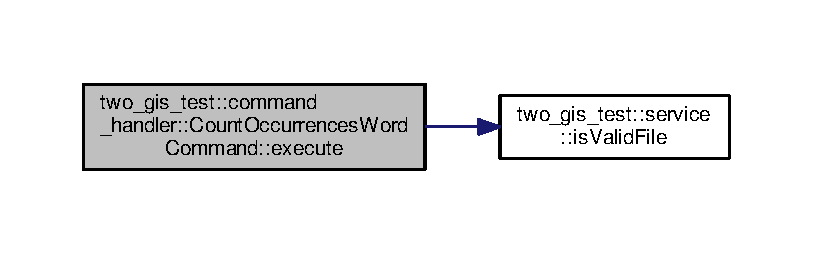
\includegraphics[width=350pt]{classtwo__gis__test_1_1command__handler_1_1_count_occurrences_word_command_a1933874918ecfc6090f8512abca372b3_cgraph}
\end{center}
\end{figure}


\index{two\+\_\+gis\+\_\+test\+::command\+\_\+handler\+::\+Count\+Occurrences\+Word\+Command@{two\+\_\+gis\+\_\+test\+::command\+\_\+handler\+::\+Count\+Occurrences\+Word\+Command}!operator=@{operator=}}
\index{operator=@{operator=}!two\+\_\+gis\+\_\+test\+::command\+\_\+handler\+::\+Count\+Occurrences\+Word\+Command@{two\+\_\+gis\+\_\+test\+::command\+\_\+handler\+::\+Count\+Occurrences\+Word\+Command}}
\subsubsection[{\texorpdfstring{operator=(const Count\+Occurrences\+Word\+Command \&)=default}{operator=(const CountOccurrencesWordCommand &)=default}}]{\setlength{\rightskip}{0pt plus 5cm}{\bf Count\+Occurrences\+Word\+Command}\& two\+\_\+gis\+\_\+test\+::command\+\_\+handler\+::\+Count\+Occurrences\+Word\+Command\+::operator= (
\begin{DoxyParamCaption}
\item[{const {\bf Count\+Occurrences\+Word\+Command} \&}]{}
\end{DoxyParamCaption}
)\hspace{0.3cm}{\ttfamily [default]}}\hypertarget{classtwo__gis__test_1_1command__handler_1_1_count_occurrences_word_command_afa3993b6f75a0090bafde445e61c1e8a}{}\label{classtwo__gis__test_1_1command__handler_1_1_count_occurrences_word_command_afa3993b6f75a0090bafde445e61c1e8a}


operator= copy assignment operator 

\index{two\+\_\+gis\+\_\+test\+::command\+\_\+handler\+::\+Count\+Occurrences\+Word\+Command@{two\+\_\+gis\+\_\+test\+::command\+\_\+handler\+::\+Count\+Occurrences\+Word\+Command}!operator=@{operator=}}
\index{operator=@{operator=}!two\+\_\+gis\+\_\+test\+::command\+\_\+handler\+::\+Count\+Occurrences\+Word\+Command@{two\+\_\+gis\+\_\+test\+::command\+\_\+handler\+::\+Count\+Occurrences\+Word\+Command}}
\subsubsection[{\texorpdfstring{operator=(\+Count\+Occurrences\+Word\+Command \&\&)=default}{operator=(CountOccurrencesWordCommand &&)=default}}]{\setlength{\rightskip}{0pt plus 5cm}{\bf Count\+Occurrences\+Word\+Command}\& two\+\_\+gis\+\_\+test\+::command\+\_\+handler\+::\+Count\+Occurrences\+Word\+Command\+::operator= (
\begin{DoxyParamCaption}
\item[{{\bf Count\+Occurrences\+Word\+Command} \&\&}]{}
\end{DoxyParamCaption}
)\hspace{0.3cm}{\ttfamily [default]}}\hypertarget{classtwo__gis__test_1_1command__handler_1_1_count_occurrences_word_command_a62e184ff22ad93cd7ff17a9c30321d11}{}\label{classtwo__gis__test_1_1command__handler_1_1_count_occurrences_word_command_a62e184ff22ad93cd7ff17a9c30321d11}


operator= move assignment operator 



The documentation for this class was generated from the following files\+:\begin{DoxyCompactItemize}
\item 
/home/boa/\+C\+Lion\+Projects/word\+\_\+counter/command\+\_\+handler/include/\hyperlink{count__occurrences__word__command_8hpp}{count\+\_\+occurrences\+\_\+word\+\_\+command.\+hpp}\item 
/home/boa/\+C\+Lion\+Projects/word\+\_\+counter/command\+\_\+handler/src/\hyperlink{count__occurrences__word__command_8cpp}{count\+\_\+occurrences\+\_\+word\+\_\+command.\+cpp}\end{DoxyCompactItemize}

\hypertarget{classtwo__gis__test_1_1command__handler_1_1_i_command}{}\section{two\+\_\+gis\+\_\+test\+:\+:command\+\_\+handler\+:\+:I\+Command Class Reference}
\label{classtwo__gis__test_1_1command__handler_1_1_i_command}\index{two\+\_\+gis\+\_\+test\+::command\+\_\+handler\+::\+I\+Command@{two\+\_\+gis\+\_\+test\+::command\+\_\+handler\+::\+I\+Command}}


{\ttfamily \#include $<$icommand.\+hpp$>$}



Inheritance diagram for two\+\_\+gis\+\_\+test\+:\+:command\+\_\+handler\+:\+:I\+Command\+:\nopagebreak
\begin{figure}[H]
\begin{center}
\leavevmode
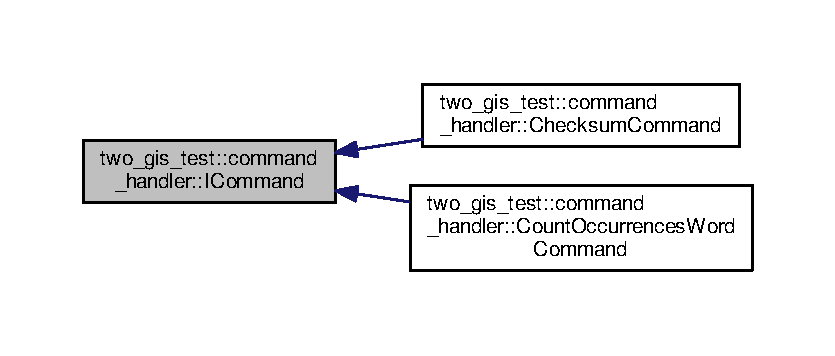
\includegraphics[width=350pt]{classtwo__gis__test_1_1command__handler_1_1_i_command__inherit__graph}
\end{center}
\end{figure}
\subsection*{Public Member Functions}
\begin{DoxyCompactItemize}
\item 
\hyperlink{classtwo__gis__test_1_1command__handler_1_1_i_command_ac6780eb9536e81697fdb4afa289f438a}{I\+Command} ()=default
\begin{DoxyCompactList}\small\item\em \hyperlink{classtwo__gis__test_1_1command__handler_1_1_i_command}{I\+Command} -\/ default constructor. \end{DoxyCompactList}\item 
virtual \hyperlink{classtwo__gis__test_1_1command__handler_1_1_i_command_a403d04e9061e1c708a7b726c2f7565dd}{$\sim$\+I\+Command} ()=default
\begin{DoxyCompactList}\small\item\em $\sim$\+I\+Command -\/ destructor \end{DoxyCompactList}\item 
\hyperlink{classtwo__gis__test_1_1command__handler_1_1_i_command_acf9cf2fcc9a9882db58d75607eb8259d}{I\+Command} (const \hyperlink{classtwo__gis__test_1_1command__handler_1_1_i_command}{I\+Command} \&)=default
\begin{DoxyCompactList}\small\item\em 
\begin{DoxyItemize}
\item copy constructor 
\end{DoxyItemize}\end{DoxyCompactList}\item 
\hyperlink{classtwo__gis__test_1_1command__handler_1_1_i_command_a07222bf1b8f0408d02abd263e6ea8b2d}{I\+Command} (\hyperlink{classtwo__gis__test_1_1command__handler_1_1_i_command}{I\+Command} \&\&)=default
\begin{DoxyCompactList}\small\item\em 
\begin{DoxyItemize}
\item move constructor 
\end{DoxyItemize}\end{DoxyCompactList}\item 
\hyperlink{classtwo__gis__test_1_1command__handler_1_1_i_command}{I\+Command} \& \hyperlink{classtwo__gis__test_1_1command__handler_1_1_i_command_aa617eba952feb604bea2a0defd9ec0c7}{operator=} (const \hyperlink{classtwo__gis__test_1_1command__handler_1_1_i_command}{I\+Command} \&)=default
\begin{DoxyCompactList}\small\item\em operator= copy assignment operator \end{DoxyCompactList}\item 
\hyperlink{classtwo__gis__test_1_1command__handler_1_1_i_command}{I\+Command} \& \hyperlink{classtwo__gis__test_1_1command__handler_1_1_i_command_a1dddaf84cffae471aa8bcd2417239f37}{operator=} (\hyperlink{classtwo__gis__test_1_1command__handler_1_1_i_command}{I\+Command} \&\&)=default
\begin{DoxyCompactList}\small\item\em operator= move assignment operator \end{DoxyCompactList}\item 
virtual void \hyperlink{classtwo__gis__test_1_1command__handler_1_1_i_command_a3674f79550d1ca7923a0c84c8fe0258f}{execute} ()=0
\begin{DoxyCompactList}\small\item\em execute -\/ pure virtual method, override in derived classes \end{DoxyCompactList}\end{DoxyCompactItemize}


\subsection{Detailed Description}
Command interface 

Definition at line 13 of file icommand.\+hpp.



\subsection{Constructor \& Destructor Documentation}
\index{two\+\_\+gis\+\_\+test\+::command\+\_\+handler\+::\+I\+Command@{two\+\_\+gis\+\_\+test\+::command\+\_\+handler\+::\+I\+Command}!I\+Command@{I\+Command}}
\index{I\+Command@{I\+Command}!two\+\_\+gis\+\_\+test\+::command\+\_\+handler\+::\+I\+Command@{two\+\_\+gis\+\_\+test\+::command\+\_\+handler\+::\+I\+Command}}
\subsubsection[{\texorpdfstring{I\+Command()=default}{ICommand()=default}}]{\setlength{\rightskip}{0pt plus 5cm}two\+\_\+gis\+\_\+test\+::command\+\_\+handler\+::\+I\+Command\+::\+I\+Command (
\begin{DoxyParamCaption}
{}
\end{DoxyParamCaption}
)\hspace{0.3cm}{\ttfamily [default]}}\hypertarget{classtwo__gis__test_1_1command__handler_1_1_i_command_ac6780eb9536e81697fdb4afa289f438a}{}\label{classtwo__gis__test_1_1command__handler_1_1_i_command_ac6780eb9536e81697fdb4afa289f438a}


\hyperlink{classtwo__gis__test_1_1command__handler_1_1_i_command}{I\+Command} -\/ default constructor. 

\index{two\+\_\+gis\+\_\+test\+::command\+\_\+handler\+::\+I\+Command@{two\+\_\+gis\+\_\+test\+::command\+\_\+handler\+::\+I\+Command}!````~I\+Command@{$\sim$\+I\+Command}}
\index{````~I\+Command@{$\sim$\+I\+Command}!two\+\_\+gis\+\_\+test\+::command\+\_\+handler\+::\+I\+Command@{two\+\_\+gis\+\_\+test\+::command\+\_\+handler\+::\+I\+Command}}
\subsubsection[{\texorpdfstring{$\sim$\+I\+Command()=default}{~ICommand()=default}}]{\setlength{\rightskip}{0pt plus 5cm}virtual two\+\_\+gis\+\_\+test\+::command\+\_\+handler\+::\+I\+Command\+::$\sim$\+I\+Command (
\begin{DoxyParamCaption}
{}
\end{DoxyParamCaption}
)\hspace{0.3cm}{\ttfamily [virtual]}, {\ttfamily [default]}}\hypertarget{classtwo__gis__test_1_1command__handler_1_1_i_command_a403d04e9061e1c708a7b726c2f7565dd}{}\label{classtwo__gis__test_1_1command__handler_1_1_i_command_a403d04e9061e1c708a7b726c2f7565dd}


$\sim$\+I\+Command -\/ destructor 

\index{two\+\_\+gis\+\_\+test\+::command\+\_\+handler\+::\+I\+Command@{two\+\_\+gis\+\_\+test\+::command\+\_\+handler\+::\+I\+Command}!I\+Command@{I\+Command}}
\index{I\+Command@{I\+Command}!two\+\_\+gis\+\_\+test\+::command\+\_\+handler\+::\+I\+Command@{two\+\_\+gis\+\_\+test\+::command\+\_\+handler\+::\+I\+Command}}
\subsubsection[{\texorpdfstring{I\+Command(const I\+Command \&)=default}{ICommand(const ICommand &)=default}}]{\setlength{\rightskip}{0pt plus 5cm}two\+\_\+gis\+\_\+test\+::command\+\_\+handler\+::\+I\+Command\+::\+I\+Command (
\begin{DoxyParamCaption}
\item[{const {\bf I\+Command} \&}]{}
\end{DoxyParamCaption}
)\hspace{0.3cm}{\ttfamily [default]}}\hypertarget{classtwo__gis__test_1_1command__handler_1_1_i_command_acf9cf2fcc9a9882db58d75607eb8259d}{}\label{classtwo__gis__test_1_1command__handler_1_1_i_command_acf9cf2fcc9a9882db58d75607eb8259d}



\begin{DoxyItemize}
\item copy constructor 
\end{DoxyItemize}

\index{two\+\_\+gis\+\_\+test\+::command\+\_\+handler\+::\+I\+Command@{two\+\_\+gis\+\_\+test\+::command\+\_\+handler\+::\+I\+Command}!I\+Command@{I\+Command}}
\index{I\+Command@{I\+Command}!two\+\_\+gis\+\_\+test\+::command\+\_\+handler\+::\+I\+Command@{two\+\_\+gis\+\_\+test\+::command\+\_\+handler\+::\+I\+Command}}
\subsubsection[{\texorpdfstring{I\+Command(\+I\+Command \&\&)=default}{ICommand(ICommand &&)=default}}]{\setlength{\rightskip}{0pt plus 5cm}two\+\_\+gis\+\_\+test\+::command\+\_\+handler\+::\+I\+Command\+::\+I\+Command (
\begin{DoxyParamCaption}
\item[{{\bf I\+Command} \&\&}]{}
\end{DoxyParamCaption}
)\hspace{0.3cm}{\ttfamily [default]}}\hypertarget{classtwo__gis__test_1_1command__handler_1_1_i_command_a07222bf1b8f0408d02abd263e6ea8b2d}{}\label{classtwo__gis__test_1_1command__handler_1_1_i_command_a07222bf1b8f0408d02abd263e6ea8b2d}



\begin{DoxyItemize}
\item move constructor 
\end{DoxyItemize}



\subsection{Member Function Documentation}
\index{two\+\_\+gis\+\_\+test\+::command\+\_\+handler\+::\+I\+Command@{two\+\_\+gis\+\_\+test\+::command\+\_\+handler\+::\+I\+Command}!execute@{execute}}
\index{execute@{execute}!two\+\_\+gis\+\_\+test\+::command\+\_\+handler\+::\+I\+Command@{two\+\_\+gis\+\_\+test\+::command\+\_\+handler\+::\+I\+Command}}
\subsubsection[{\texorpdfstring{execute()=0}{execute()=0}}]{\setlength{\rightskip}{0pt plus 5cm}virtual void two\+\_\+gis\+\_\+test\+::command\+\_\+handler\+::\+I\+Command\+::execute (
\begin{DoxyParamCaption}
{}
\end{DoxyParamCaption}
)\hspace{0.3cm}{\ttfamily [pure virtual]}}\hypertarget{classtwo__gis__test_1_1command__handler_1_1_i_command_a3674f79550d1ca7923a0c84c8fe0258f}{}\label{classtwo__gis__test_1_1command__handler_1_1_i_command_a3674f79550d1ca7923a0c84c8fe0258f}


execute -\/ pure virtual method, override in derived classes 



Implemented in \hyperlink{classtwo__gis__test_1_1command__handler_1_1_count_occurrences_word_command_a1933874918ecfc6090f8512abca372b3}{two\+\_\+gis\+\_\+test\+::command\+\_\+handler\+::\+Count\+Occurrences\+Word\+Command}, and \hyperlink{classtwo__gis__test_1_1command__handler_1_1_checksum_command_a3ab082ac86155aa117e9870011a791f2}{two\+\_\+gis\+\_\+test\+::command\+\_\+handler\+::\+Checksum\+Command}.

\index{two\+\_\+gis\+\_\+test\+::command\+\_\+handler\+::\+I\+Command@{two\+\_\+gis\+\_\+test\+::command\+\_\+handler\+::\+I\+Command}!operator=@{operator=}}
\index{operator=@{operator=}!two\+\_\+gis\+\_\+test\+::command\+\_\+handler\+::\+I\+Command@{two\+\_\+gis\+\_\+test\+::command\+\_\+handler\+::\+I\+Command}}
\subsubsection[{\texorpdfstring{operator=(const I\+Command \&)=default}{operator=(const ICommand &)=default}}]{\setlength{\rightskip}{0pt plus 5cm}{\bf I\+Command}\& two\+\_\+gis\+\_\+test\+::command\+\_\+handler\+::\+I\+Command\+::operator= (
\begin{DoxyParamCaption}
\item[{const {\bf I\+Command} \&}]{}
\end{DoxyParamCaption}
)\hspace{0.3cm}{\ttfamily [default]}}\hypertarget{classtwo__gis__test_1_1command__handler_1_1_i_command_aa617eba952feb604bea2a0defd9ec0c7}{}\label{classtwo__gis__test_1_1command__handler_1_1_i_command_aa617eba952feb604bea2a0defd9ec0c7}


operator= copy assignment operator 

\index{two\+\_\+gis\+\_\+test\+::command\+\_\+handler\+::\+I\+Command@{two\+\_\+gis\+\_\+test\+::command\+\_\+handler\+::\+I\+Command}!operator=@{operator=}}
\index{operator=@{operator=}!two\+\_\+gis\+\_\+test\+::command\+\_\+handler\+::\+I\+Command@{two\+\_\+gis\+\_\+test\+::command\+\_\+handler\+::\+I\+Command}}
\subsubsection[{\texorpdfstring{operator=(\+I\+Command \&\&)=default}{operator=(ICommand &&)=default}}]{\setlength{\rightskip}{0pt plus 5cm}{\bf I\+Command}\& two\+\_\+gis\+\_\+test\+::command\+\_\+handler\+::\+I\+Command\+::operator= (
\begin{DoxyParamCaption}
\item[{{\bf I\+Command} \&\&}]{}
\end{DoxyParamCaption}
)\hspace{0.3cm}{\ttfamily [default]}}\hypertarget{classtwo__gis__test_1_1command__handler_1_1_i_command_a1dddaf84cffae471aa8bcd2417239f37}{}\label{classtwo__gis__test_1_1command__handler_1_1_i_command_a1dddaf84cffae471aa8bcd2417239f37}


operator= move assignment operator 



The documentation for this class was generated from the following file\+:\begin{DoxyCompactItemize}
\item 
/home/boa/\+C\+Lion\+Projects/word\+\_\+counter/command\+\_\+handler/include/\hyperlink{icommand_8hpp}{icommand.\+hpp}\end{DoxyCompactItemize}

\hypertarget{classtwo__gis__test_1_1command__handler_1_1_invoker}{}\section{two\+\_\+gis\+\_\+test\+:\+:command\+\_\+handler\+:\+:Invoker Class Reference}
\label{classtwo__gis__test_1_1command__handler_1_1_invoker}\index{two\+\_\+gis\+\_\+test\+::command\+\_\+handler\+::\+Invoker@{two\+\_\+gis\+\_\+test\+::command\+\_\+handler\+::\+Invoker}}


{\ttfamily \#include $<$invoker.\+hpp$>$}

\subsection*{Public Member Functions}
\begin{DoxyCompactItemize}
\item 
\hyperlink{classtwo__gis__test_1_1command__handler_1_1_invoker_a18951d9324c7b97c0f4652591cbafb97}{Invoker} ()=default
\begin{DoxyCompactList}\small\item\em \hyperlink{classtwo__gis__test_1_1command__handler_1_1_invoker}{Invoker} -\/ constructor. \end{DoxyCompactList}\item 
virtual \hyperlink{classtwo__gis__test_1_1command__handler_1_1_invoker_ab6aec58f3120f3c5fe7d6cc75d5d2fa8}{$\sim$\+Invoker} ()=default
\begin{DoxyCompactList}\small\item\em $\sim$\+Invoker -\/ destructor \end{DoxyCompactList}\item 
\hyperlink{classtwo__gis__test_1_1command__handler_1_1_invoker_aa7ea20637e71826d4287050fc5d7ec49}{Invoker} (const \hyperlink{classtwo__gis__test_1_1command__handler_1_1_invoker}{Invoker} \&)=default
\begin{DoxyCompactList}\small\item\em \hyperlink{classtwo__gis__test_1_1command__handler_1_1_invoker}{Invoker} -\/ copy contructor. \end{DoxyCompactList}\item 
\hyperlink{classtwo__gis__test_1_1command__handler_1_1_invoker_aa6dc501d5aba59816c3167a04bc6ef18}{Invoker} (\hyperlink{classtwo__gis__test_1_1command__handler_1_1_invoker}{Invoker} \&\&)=default
\begin{DoxyCompactList}\small\item\em \hyperlink{classtwo__gis__test_1_1command__handler_1_1_invoker}{Invoker} -\/ move constructor. \end{DoxyCompactList}\item 
\hyperlink{classtwo__gis__test_1_1command__handler_1_1_invoker}{Invoker} \& \hyperlink{classtwo__gis__test_1_1command__handler_1_1_invoker_ab0f46886672dd682e4c3da7de24afb16}{operator=} (const \hyperlink{classtwo__gis__test_1_1command__handler_1_1_invoker}{Invoker} \&)=default
\begin{DoxyCompactList}\small\item\em operator= -\/ copy assignment operator \end{DoxyCompactList}\item 
\hyperlink{classtwo__gis__test_1_1command__handler_1_1_invoker}{Invoker} \& \hyperlink{classtwo__gis__test_1_1command__handler_1_1_invoker_a0e5ad5a769bf4ad41793ef577fbd36f7}{operator=} (\hyperlink{classtwo__gis__test_1_1command__handler_1_1_invoker}{Invoker} \&\&)=default
\begin{DoxyCompactList}\small\item\em operator= move assignment operator \end{DoxyCompactList}\item 
void \hyperlink{classtwo__gis__test_1_1command__handler_1_1_invoker_aa883eef9d0cdc7d9d2b299a656fc0dc0}{count\+Occurrences\+Word} (std\+::string \&filename, std\+::string \&search\+Word)
\begin{DoxyCompactList}\small\item\em count\+Occurrences\+Word -\/ create \hyperlink{classtwo__gis__test_1_1command__handler_1_1_count_occurrences_word_command}{Count\+Occurrences\+Word\+Command} and send to \hyperlink{classtwo__gis__test_1_1command__handler_1_1_command_handler}{Command\+Handler} \end{DoxyCompactList}\item 
void \hyperlink{classtwo__gis__test_1_1command__handler_1_1_invoker_ae8fcf1764c98033f7fe855f4924eab7f}{calculate\+Check\+Sum} (std\+::string \&filename)
\begin{DoxyCompactList}\small\item\em calculate\+Check\+Sum -\/ create \hyperlink{classtwo__gis__test_1_1command__handler_1_1_checksum_command}{Checksum\+Command} and sent to \hyperlink{classtwo__gis__test_1_1command__handler_1_1_command_handler}{Command\+Handler} \end{DoxyCompactList}\end{DoxyCompactItemize}
\subsection*{Public Attributes}
\begin{DoxyCompactItemize}
\item 
boost\+::signals2\+::signal$<$ void(std\+::shared\+\_\+ptr$<$ \hyperlink{classtwo__gis__test_1_1command__handler_1_1_i_command}{I\+Command} $>$ command)$>$ \hyperlink{classtwo__gis__test_1_1command__handler_1_1_invoker_a93519fc81bdc3f6e1832c6e3c1b5ad3a}{start}
\begin{DoxyCompactList}\small\item\em start -\/ boost signal for sending command to \hyperlink{classtwo__gis__test_1_1command__handler_1_1_command_handler}{Command\+Handler} \end{DoxyCompactList}\end{DoxyCompactItemize}
\subsection*{Protected Member Functions}
\begin{DoxyCompactItemize}
\item 
std\+::shared\+\_\+ptr$<$ \hyperlink{classtwo__gis__test_1_1command__handler_1_1_i_command}{I\+Command} $>$ \hyperlink{classtwo__gis__test_1_1command__handler_1_1_invoker_aaa8657d1d2b7724976ddbaca0817415d}{create\+Count\+Occurrences\+Word\+Command} (std\+::string \&filename, std\+::string \&search\+Word)
\begin{DoxyCompactList}\small\item\em create\+Count\+Occurrences\+Word\+Command -\/ create new exemplar of \hyperlink{classtwo__gis__test_1_1command__handler_1_1_count_occurrences_word_command}{Count\+Occurrences\+Word\+Command} class \end{DoxyCompactList}\item 
std\+::shared\+\_\+ptr$<$ \hyperlink{classtwo__gis__test_1_1command__handler_1_1_i_command}{I\+Command} $>$ \hyperlink{classtwo__gis__test_1_1command__handler_1_1_invoker_a9ad77345397bfea08fe5319388fcd91a}{create\+Checksum\+Command} (std\+::string \&filename)
\begin{DoxyCompactList}\small\item\em create\+Checksum\+Command -\/ create new exemplar of \hyperlink{classtwo__gis__test_1_1command__handler_1_1_checksum_command}{Checksum\+Command} class \end{DoxyCompactList}\end{DoxyCompactItemize}


\subsection{Detailed Description}
on the input data received from the client, it generates commands and passes it on to execution 

Definition at line 19 of file invoker.\+hpp.



\subsection{Constructor \& Destructor Documentation}
\index{two\+\_\+gis\+\_\+test\+::command\+\_\+handler\+::\+Invoker@{two\+\_\+gis\+\_\+test\+::command\+\_\+handler\+::\+Invoker}!Invoker@{Invoker}}
\index{Invoker@{Invoker}!two\+\_\+gis\+\_\+test\+::command\+\_\+handler\+::\+Invoker@{two\+\_\+gis\+\_\+test\+::command\+\_\+handler\+::\+Invoker}}
\subsubsection[{\texorpdfstring{Invoker()=default}{Invoker()=default}}]{\setlength{\rightskip}{0pt plus 5cm}two\+\_\+gis\+\_\+test\+::command\+\_\+handler\+::\+Invoker\+::\+Invoker (
\begin{DoxyParamCaption}
{}
\end{DoxyParamCaption}
)\hspace{0.3cm}{\ttfamily [default]}}\hypertarget{classtwo__gis__test_1_1command__handler_1_1_invoker_a18951d9324c7b97c0f4652591cbafb97}{}\label{classtwo__gis__test_1_1command__handler_1_1_invoker_a18951d9324c7b97c0f4652591cbafb97}


\hyperlink{classtwo__gis__test_1_1command__handler_1_1_invoker}{Invoker} -\/ constructor. 

\index{two\+\_\+gis\+\_\+test\+::command\+\_\+handler\+::\+Invoker@{two\+\_\+gis\+\_\+test\+::command\+\_\+handler\+::\+Invoker}!````~Invoker@{$\sim$\+Invoker}}
\index{````~Invoker@{$\sim$\+Invoker}!two\+\_\+gis\+\_\+test\+::command\+\_\+handler\+::\+Invoker@{two\+\_\+gis\+\_\+test\+::command\+\_\+handler\+::\+Invoker}}
\subsubsection[{\texorpdfstring{$\sim$\+Invoker()=default}{~Invoker()=default}}]{\setlength{\rightskip}{0pt plus 5cm}virtual two\+\_\+gis\+\_\+test\+::command\+\_\+handler\+::\+Invoker\+::$\sim$\+Invoker (
\begin{DoxyParamCaption}
{}
\end{DoxyParamCaption}
)\hspace{0.3cm}{\ttfamily [virtual]}, {\ttfamily [default]}}\hypertarget{classtwo__gis__test_1_1command__handler_1_1_invoker_ab6aec58f3120f3c5fe7d6cc75d5d2fa8}{}\label{classtwo__gis__test_1_1command__handler_1_1_invoker_ab6aec58f3120f3c5fe7d6cc75d5d2fa8}


$\sim$\+Invoker -\/ destructor 

\index{two\+\_\+gis\+\_\+test\+::command\+\_\+handler\+::\+Invoker@{two\+\_\+gis\+\_\+test\+::command\+\_\+handler\+::\+Invoker}!Invoker@{Invoker}}
\index{Invoker@{Invoker}!two\+\_\+gis\+\_\+test\+::command\+\_\+handler\+::\+Invoker@{two\+\_\+gis\+\_\+test\+::command\+\_\+handler\+::\+Invoker}}
\subsubsection[{\texorpdfstring{Invoker(const Invoker \&)=default}{Invoker(const Invoker &)=default}}]{\setlength{\rightskip}{0pt plus 5cm}two\+\_\+gis\+\_\+test\+::command\+\_\+handler\+::\+Invoker\+::\+Invoker (
\begin{DoxyParamCaption}
\item[{const {\bf Invoker} \&}]{}
\end{DoxyParamCaption}
)\hspace{0.3cm}{\ttfamily [default]}}\hypertarget{classtwo__gis__test_1_1command__handler_1_1_invoker_aa7ea20637e71826d4287050fc5d7ec49}{}\label{classtwo__gis__test_1_1command__handler_1_1_invoker_aa7ea20637e71826d4287050fc5d7ec49}


\hyperlink{classtwo__gis__test_1_1command__handler_1_1_invoker}{Invoker} -\/ copy contructor. 

\index{two\+\_\+gis\+\_\+test\+::command\+\_\+handler\+::\+Invoker@{two\+\_\+gis\+\_\+test\+::command\+\_\+handler\+::\+Invoker}!Invoker@{Invoker}}
\index{Invoker@{Invoker}!two\+\_\+gis\+\_\+test\+::command\+\_\+handler\+::\+Invoker@{two\+\_\+gis\+\_\+test\+::command\+\_\+handler\+::\+Invoker}}
\subsubsection[{\texorpdfstring{Invoker(\+Invoker \&\&)=default}{Invoker(Invoker &&)=default}}]{\setlength{\rightskip}{0pt plus 5cm}two\+\_\+gis\+\_\+test\+::command\+\_\+handler\+::\+Invoker\+::\+Invoker (
\begin{DoxyParamCaption}
\item[{{\bf Invoker} \&\&}]{}
\end{DoxyParamCaption}
)\hspace{0.3cm}{\ttfamily [default]}}\hypertarget{classtwo__gis__test_1_1command__handler_1_1_invoker_aa6dc501d5aba59816c3167a04bc6ef18}{}\label{classtwo__gis__test_1_1command__handler_1_1_invoker_aa6dc501d5aba59816c3167a04bc6ef18}


\hyperlink{classtwo__gis__test_1_1command__handler_1_1_invoker}{Invoker} -\/ move constructor. 



\subsection{Member Function Documentation}
\index{two\+\_\+gis\+\_\+test\+::command\+\_\+handler\+::\+Invoker@{two\+\_\+gis\+\_\+test\+::command\+\_\+handler\+::\+Invoker}!calculate\+Check\+Sum@{calculate\+Check\+Sum}}
\index{calculate\+Check\+Sum@{calculate\+Check\+Sum}!two\+\_\+gis\+\_\+test\+::command\+\_\+handler\+::\+Invoker@{two\+\_\+gis\+\_\+test\+::command\+\_\+handler\+::\+Invoker}}
\subsubsection[{\texorpdfstring{calculate\+Check\+Sum(std\+::string \&filename)}{calculateCheckSum(std::string &filename)}}]{\setlength{\rightskip}{0pt plus 5cm}void two\+\_\+gis\+\_\+test\+::command\+\_\+handler\+::\+Invoker\+::calculate\+Check\+Sum (
\begin{DoxyParamCaption}
\item[{std\+::string \&}]{filename}
\end{DoxyParamCaption}
)}\hypertarget{classtwo__gis__test_1_1command__handler_1_1_invoker_ae8fcf1764c98033f7fe855f4924eab7f}{}\label{classtwo__gis__test_1_1command__handler_1_1_invoker_ae8fcf1764c98033f7fe855f4924eab7f}


calculate\+Check\+Sum -\/ create \hyperlink{classtwo__gis__test_1_1command__handler_1_1_checksum_command}{Checksum\+Command} and sent to \hyperlink{classtwo__gis__test_1_1command__handler_1_1_command_handler}{Command\+Handler} 


\begin{DoxyParams}{Parameters}
{\em filename} & -\/ input file \\
\hline
\end{DoxyParams}


Definition at line 26 of file invoker.\+cpp.



Here is the call graph for this function\+:\nopagebreak
\begin{figure}[H]
\begin{center}
\leavevmode
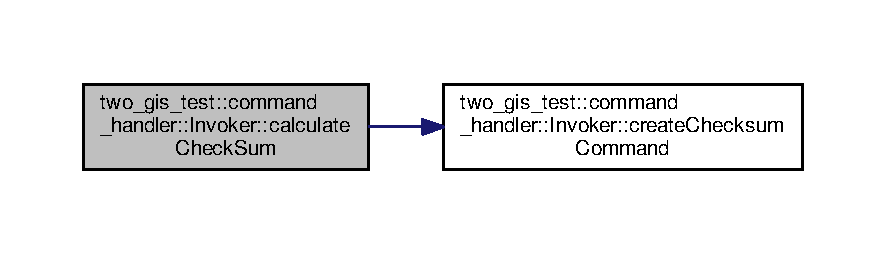
\includegraphics[width=350pt]{classtwo__gis__test_1_1command__handler_1_1_invoker_ae8fcf1764c98033f7fe855f4924eab7f_cgraph}
\end{center}
\end{figure}


\index{two\+\_\+gis\+\_\+test\+::command\+\_\+handler\+::\+Invoker@{two\+\_\+gis\+\_\+test\+::command\+\_\+handler\+::\+Invoker}!count\+Occurrences\+Word@{count\+Occurrences\+Word}}
\index{count\+Occurrences\+Word@{count\+Occurrences\+Word}!two\+\_\+gis\+\_\+test\+::command\+\_\+handler\+::\+Invoker@{two\+\_\+gis\+\_\+test\+::command\+\_\+handler\+::\+Invoker}}
\subsubsection[{\texorpdfstring{count\+Occurrences\+Word(std\+::string \&filename, std\+::string \&search\+Word)}{countOccurrencesWord(std::string &filename, std::string &searchWord)}}]{\setlength{\rightskip}{0pt plus 5cm}void two\+\_\+gis\+\_\+test\+::command\+\_\+handler\+::\+Invoker\+::count\+Occurrences\+Word (
\begin{DoxyParamCaption}
\item[{std\+::string \&}]{filename, }
\item[{std\+::string \&}]{search\+Word}
\end{DoxyParamCaption}
)}\hypertarget{classtwo__gis__test_1_1command__handler_1_1_invoker_aa883eef9d0cdc7d9d2b299a656fc0dc0}{}\label{classtwo__gis__test_1_1command__handler_1_1_invoker_aa883eef9d0cdc7d9d2b299a656fc0dc0}


count\+Occurrences\+Word -\/ create \hyperlink{classtwo__gis__test_1_1command__handler_1_1_count_occurrences_word_command}{Count\+Occurrences\+Word\+Command} and send to \hyperlink{classtwo__gis__test_1_1command__handler_1_1_command_handler}{Command\+Handler} 


\begin{DoxyParams}{Parameters}
{\em filename} & -\/ input file \\
\hline
{\em search\+Word} & -\/ word, the number of occurrences of which will be calculated \\
\hline
\end{DoxyParams}


Definition at line 21 of file invoker.\+cpp.



Here is the call graph for this function\+:\nopagebreak
\begin{figure}[H]
\begin{center}
\leavevmode
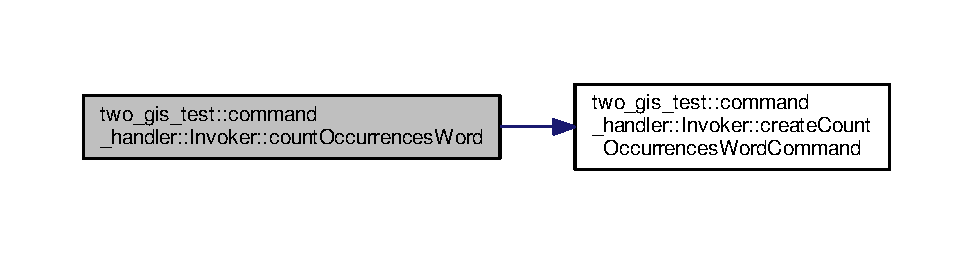
\includegraphics[width=350pt]{classtwo__gis__test_1_1command__handler_1_1_invoker_aa883eef9d0cdc7d9d2b299a656fc0dc0_cgraph}
\end{center}
\end{figure}


\index{two\+\_\+gis\+\_\+test\+::command\+\_\+handler\+::\+Invoker@{two\+\_\+gis\+\_\+test\+::command\+\_\+handler\+::\+Invoker}!create\+Checksum\+Command@{create\+Checksum\+Command}}
\index{create\+Checksum\+Command@{create\+Checksum\+Command}!two\+\_\+gis\+\_\+test\+::command\+\_\+handler\+::\+Invoker@{two\+\_\+gis\+\_\+test\+::command\+\_\+handler\+::\+Invoker}}
\subsubsection[{\texorpdfstring{create\+Checksum\+Command(std\+::string \&filename)}{createChecksumCommand(std::string &filename)}}]{\setlength{\rightskip}{0pt plus 5cm}std\+::shared\+\_\+ptr$<$ {\bf I\+Command} $>$ two\+\_\+gis\+\_\+test\+::command\+\_\+handler\+::\+Invoker\+::create\+Checksum\+Command (
\begin{DoxyParamCaption}
\item[{std\+::string \&}]{filename}
\end{DoxyParamCaption}
)\hspace{0.3cm}{\ttfamily [protected]}}\hypertarget{classtwo__gis__test_1_1command__handler_1_1_invoker_a9ad77345397bfea08fe5319388fcd91a}{}\label{classtwo__gis__test_1_1command__handler_1_1_invoker_a9ad77345397bfea08fe5319388fcd91a}


create\+Checksum\+Command -\/ create new exemplar of \hyperlink{classtwo__gis__test_1_1command__handler_1_1_checksum_command}{Checksum\+Command} class 


\begin{DoxyParams}{Parameters}
{\em filename} & -\/ input file \\
\hline
\end{DoxyParams}
\begin{DoxyReturn}{Returns}
new exemplar of \hyperlink{classtwo__gis__test_1_1command__handler_1_1_checksum_command}{Checksum\+Command} class 
\end{DoxyReturn}


Definition at line 17 of file invoker.\+cpp.



Here is the caller graph for this function\+:\nopagebreak
\begin{figure}[H]
\begin{center}
\leavevmode
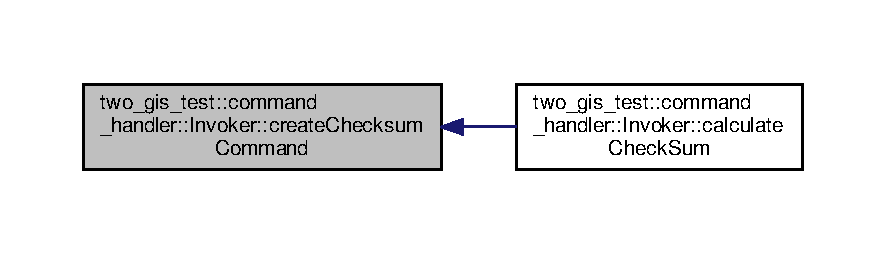
\includegraphics[width=350pt]{classtwo__gis__test_1_1command__handler_1_1_invoker_a9ad77345397bfea08fe5319388fcd91a_icgraph}
\end{center}
\end{figure}


\index{two\+\_\+gis\+\_\+test\+::command\+\_\+handler\+::\+Invoker@{two\+\_\+gis\+\_\+test\+::command\+\_\+handler\+::\+Invoker}!create\+Count\+Occurrences\+Word\+Command@{create\+Count\+Occurrences\+Word\+Command}}
\index{create\+Count\+Occurrences\+Word\+Command@{create\+Count\+Occurrences\+Word\+Command}!two\+\_\+gis\+\_\+test\+::command\+\_\+handler\+::\+Invoker@{two\+\_\+gis\+\_\+test\+::command\+\_\+handler\+::\+Invoker}}
\subsubsection[{\texorpdfstring{create\+Count\+Occurrences\+Word\+Command(std\+::string \&filename, std\+::string \&search\+Word)}{createCountOccurrencesWordCommand(std::string &filename, std::string &searchWord)}}]{\setlength{\rightskip}{0pt plus 5cm}std\+::shared\+\_\+ptr$<$ {\bf I\+Command} $>$ two\+\_\+gis\+\_\+test\+::command\+\_\+handler\+::\+Invoker\+::create\+Count\+Occurrences\+Word\+Command (
\begin{DoxyParamCaption}
\item[{std\+::string \&}]{filename, }
\item[{std\+::string \&}]{search\+Word}
\end{DoxyParamCaption}
)\hspace{0.3cm}{\ttfamily [protected]}}\hypertarget{classtwo__gis__test_1_1command__handler_1_1_invoker_aaa8657d1d2b7724976ddbaca0817415d}{}\label{classtwo__gis__test_1_1command__handler_1_1_invoker_aaa8657d1d2b7724976ddbaca0817415d}


create\+Count\+Occurrences\+Word\+Command -\/ create new exemplar of \hyperlink{classtwo__gis__test_1_1command__handler_1_1_count_occurrences_word_command}{Count\+Occurrences\+Word\+Command} class 


\begin{DoxyParams}{Parameters}
{\em filename} & -\/ input file \\
\hline
{\em search\+Word} & -\/ Word, the number of occurrences of which will be calculated \\
\hline
\end{DoxyParams}
\begin{DoxyReturn}{Returns}
-\/ new exemplar of \hyperlink{classtwo__gis__test_1_1command__handler_1_1_count_occurrences_word_command}{Count\+Occurrences\+Word\+Command} class 
\end{DoxyReturn}


Definition at line 12 of file invoker.\+cpp.



Here is the caller graph for this function\+:\nopagebreak
\begin{figure}[H]
\begin{center}
\leavevmode
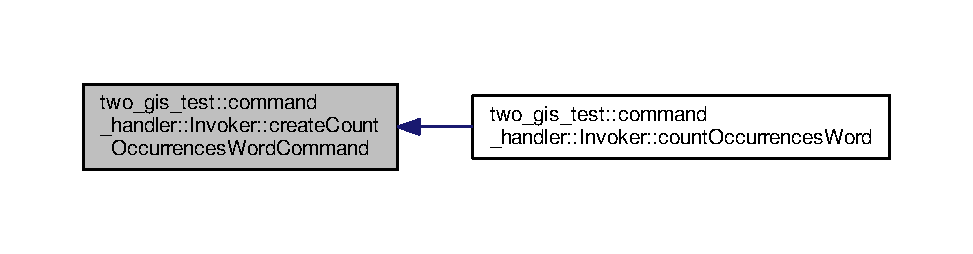
\includegraphics[width=350pt]{classtwo__gis__test_1_1command__handler_1_1_invoker_aaa8657d1d2b7724976ddbaca0817415d_icgraph}
\end{center}
\end{figure}


\index{two\+\_\+gis\+\_\+test\+::command\+\_\+handler\+::\+Invoker@{two\+\_\+gis\+\_\+test\+::command\+\_\+handler\+::\+Invoker}!operator=@{operator=}}
\index{operator=@{operator=}!two\+\_\+gis\+\_\+test\+::command\+\_\+handler\+::\+Invoker@{two\+\_\+gis\+\_\+test\+::command\+\_\+handler\+::\+Invoker}}
\subsubsection[{\texorpdfstring{operator=(const Invoker \&)=default}{operator=(const Invoker &)=default}}]{\setlength{\rightskip}{0pt plus 5cm}{\bf Invoker}\& two\+\_\+gis\+\_\+test\+::command\+\_\+handler\+::\+Invoker\+::operator= (
\begin{DoxyParamCaption}
\item[{const {\bf Invoker} \&}]{}
\end{DoxyParamCaption}
)\hspace{0.3cm}{\ttfamily [default]}}\hypertarget{classtwo__gis__test_1_1command__handler_1_1_invoker_ab0f46886672dd682e4c3da7de24afb16}{}\label{classtwo__gis__test_1_1command__handler_1_1_invoker_ab0f46886672dd682e4c3da7de24afb16}


operator= -\/ copy assignment operator 

\index{two\+\_\+gis\+\_\+test\+::command\+\_\+handler\+::\+Invoker@{two\+\_\+gis\+\_\+test\+::command\+\_\+handler\+::\+Invoker}!operator=@{operator=}}
\index{operator=@{operator=}!two\+\_\+gis\+\_\+test\+::command\+\_\+handler\+::\+Invoker@{two\+\_\+gis\+\_\+test\+::command\+\_\+handler\+::\+Invoker}}
\subsubsection[{\texorpdfstring{operator=(\+Invoker \&\&)=default}{operator=(Invoker &&)=default}}]{\setlength{\rightskip}{0pt plus 5cm}{\bf Invoker}\& two\+\_\+gis\+\_\+test\+::command\+\_\+handler\+::\+Invoker\+::operator= (
\begin{DoxyParamCaption}
\item[{{\bf Invoker} \&\&}]{}
\end{DoxyParamCaption}
)\hspace{0.3cm}{\ttfamily [default]}}\hypertarget{classtwo__gis__test_1_1command__handler_1_1_invoker_a0e5ad5a769bf4ad41793ef577fbd36f7}{}\label{classtwo__gis__test_1_1command__handler_1_1_invoker_a0e5ad5a769bf4ad41793ef577fbd36f7}


operator= move assignment operator 



\subsection{Member Data Documentation}
\index{two\+\_\+gis\+\_\+test\+::command\+\_\+handler\+::\+Invoker@{two\+\_\+gis\+\_\+test\+::command\+\_\+handler\+::\+Invoker}!start@{start}}
\index{start@{start}!two\+\_\+gis\+\_\+test\+::command\+\_\+handler\+::\+Invoker@{two\+\_\+gis\+\_\+test\+::command\+\_\+handler\+::\+Invoker}}
\subsubsection[{\texorpdfstring{start}{start}}]{\setlength{\rightskip}{0pt plus 5cm}boost\+::signals2\+::signal$<$void(std\+::shared\+\_\+ptr$<${\bf I\+Command}$>$ command)$>$ two\+\_\+gis\+\_\+test\+::command\+\_\+handler\+::\+Invoker\+::start}\hypertarget{classtwo__gis__test_1_1command__handler_1_1_invoker_a93519fc81bdc3f6e1832c6e3c1b5ad3a}{}\label{classtwo__gis__test_1_1command__handler_1_1_invoker_a93519fc81bdc3f6e1832c6e3c1b5ad3a}


start -\/ boost signal for sending command to \hyperlink{classtwo__gis__test_1_1command__handler_1_1_command_handler}{Command\+Handler} 



Definition at line 67 of file invoker.\+hpp.



The documentation for this class was generated from the following files\+:\begin{DoxyCompactItemize}
\item 
/home/boa/\+C\+Lion\+Projects/word\+\_\+counter/command\+\_\+handler/include/\hyperlink{invoker_8hpp}{invoker.\+hpp}\item 
/home/boa/\+C\+Lion\+Projects/word\+\_\+counter/command\+\_\+handler/src/\hyperlink{invoker_8cpp}{invoker.\+cpp}\end{DoxyCompactItemize}

\chapter{File Documentation}
\hypertarget{args__parse__exception_8hpp}{}\section{/home/boa/\+C\+Lion\+Projects/word\+\_\+counter/args\+\_\+parser/include/args\+\_\+parse\+\_\+exception.hpp File Reference}
\label{args__parse__exception_8hpp}\index{/home/boa/\+C\+Lion\+Projects/word\+\_\+counter/args\+\_\+parser/include/args\+\_\+parse\+\_\+exception.\+hpp@{/home/boa/\+C\+Lion\+Projects/word\+\_\+counter/args\+\_\+parser/include/args\+\_\+parse\+\_\+exception.\+hpp}}
{\ttfamily \#include $<$exception$>$}\\*
{\ttfamily \#include $<$string$>$}\\*
Include dependency graph for args\+\_\+parse\+\_\+exception.\+hpp\+:\nopagebreak
\begin{figure}[H]
\begin{center}
\leavevmode
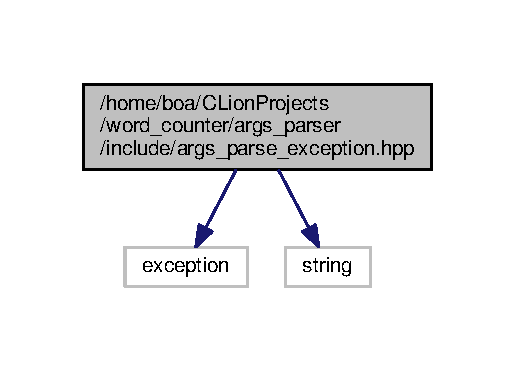
\includegraphics[width=247pt]{args__parse__exception_8hpp__incl}
\end{center}
\end{figure}
This graph shows which files directly or indirectly include this file\+:\nopagebreak
\begin{figure}[H]
\begin{center}
\leavevmode
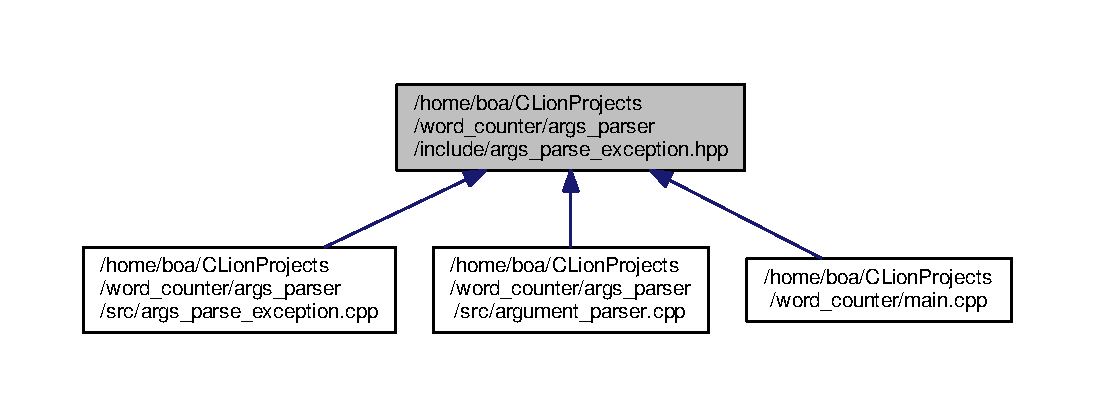
\includegraphics[width=350pt]{args__parse__exception_8hpp__dep__incl}
\end{center}
\end{figure}
\subsection*{Classes}
\begin{DoxyCompactItemize}
\item 
class \hyperlink{classtwo__gis__test_1_1argument__parser_1_1_args_parse_exception}{two\+\_\+gis\+\_\+test\+::argument\+\_\+parser\+::\+Args\+Parse\+Exception}
\end{DoxyCompactItemize}
\subsection*{Namespaces}
\begin{DoxyCompactItemize}
\item 
 \hyperlink{namespacetwo__gis__test}{two\+\_\+gis\+\_\+test}
\item 
 \hyperlink{namespacetwo__gis__test_1_1argument__parser}{two\+\_\+gis\+\_\+test\+::argument\+\_\+parser}
\end{DoxyCompactItemize}

\hypertarget{argument__parser_8hpp}{}\section{/home/boa/\+C\+Lion\+Projects/word\+\_\+counter/args\+\_\+parser/include/argument\+\_\+parser.hpp File Reference}
\label{argument__parser_8hpp}\index{/home/boa/\+C\+Lion\+Projects/word\+\_\+counter/args\+\_\+parser/include/argument\+\_\+parser.\+hpp@{/home/boa/\+C\+Lion\+Projects/word\+\_\+counter/args\+\_\+parser/include/argument\+\_\+parser.\+hpp}}
{\ttfamily \#include $<$boost/program\+\_\+options.\+hpp$>$}\\*
{\ttfamily \#include $<$boost/signals2.\+hpp$>$}\\*
{\ttfamily \#include $<$boost/filesystem.\+hpp$>$}\\*
{\ttfamily \#include $<$iostream$>$}\\*
{\ttfamily \#include \char`\"{}../../service/include/service.\+hpp\char`\"{}}\\*
Include dependency graph for argument\+\_\+parser.\+hpp\+:\nopagebreak
\begin{figure}[H]
\begin{center}
\leavevmode
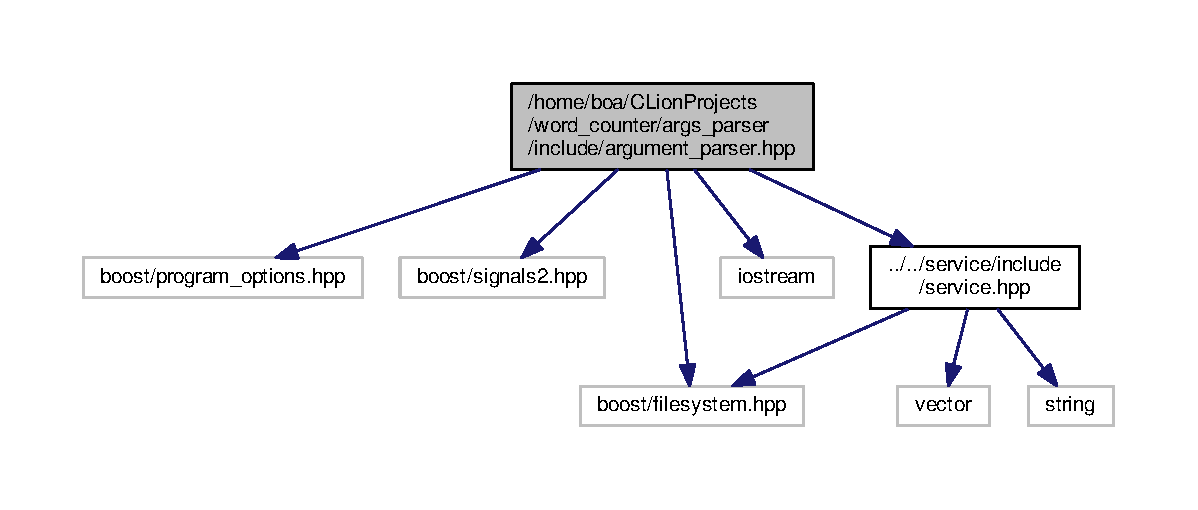
\includegraphics[width=350pt]{argument__parser_8hpp__incl}
\end{center}
\end{figure}
This graph shows which files directly or indirectly include this file\+:\nopagebreak
\begin{figure}[H]
\begin{center}
\leavevmode
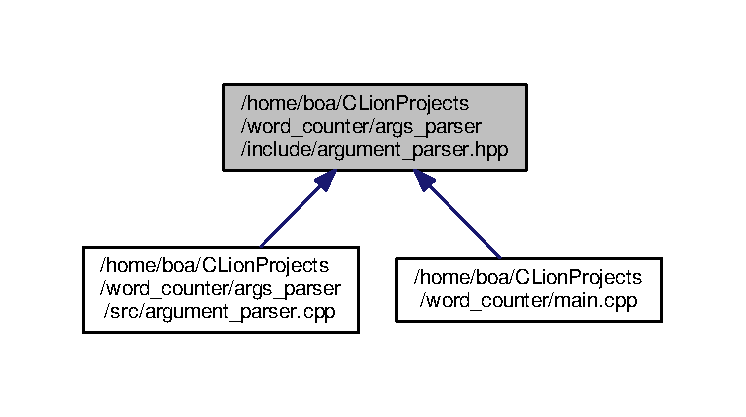
\includegraphics[width=350pt]{argument__parser_8hpp__dep__incl}
\end{center}
\end{figure}
\subsection*{Classes}
\begin{DoxyCompactItemize}
\item 
class \hyperlink{classtwo__gis__test_1_1argument__parser_1_1_argument_parser}{two\+\_\+gis\+\_\+test\+::argument\+\_\+parser\+::\+Argument\+Parser}
\end{DoxyCompactItemize}
\subsection*{Namespaces}
\begin{DoxyCompactItemize}
\item 
 \hyperlink{namespacetwo__gis__test}{two\+\_\+gis\+\_\+test}
\item 
 \hyperlink{namespacetwo__gis__test_1_1argument__parser}{two\+\_\+gis\+\_\+test\+::argument\+\_\+parser}
\end{DoxyCompactItemize}

\hypertarget{args__parse__exception_8cpp}{}\section{/home/boa/\+C\+Lion\+Projects/word\+\_\+counter/args\+\_\+parser/src/args\+\_\+parse\+\_\+exception.cpp File Reference}
\label{args__parse__exception_8cpp}\index{/home/boa/\+C\+Lion\+Projects/word\+\_\+counter/args\+\_\+parser/src/args\+\_\+parse\+\_\+exception.\+cpp@{/home/boa/\+C\+Lion\+Projects/word\+\_\+counter/args\+\_\+parser/src/args\+\_\+parse\+\_\+exception.\+cpp}}
{\ttfamily \#include $<$cstring$>$}\\*
{\ttfamily \#include $<$memory$>$}\\*
{\ttfamily \#include \char`\"{}../include/args\+\_\+parse\+\_\+exception.\+hpp\char`\"{}}\\*
Include dependency graph for args\+\_\+parse\+\_\+exception.\+cpp\+:\nopagebreak
\begin{figure}[H]
\begin{center}
\leavevmode
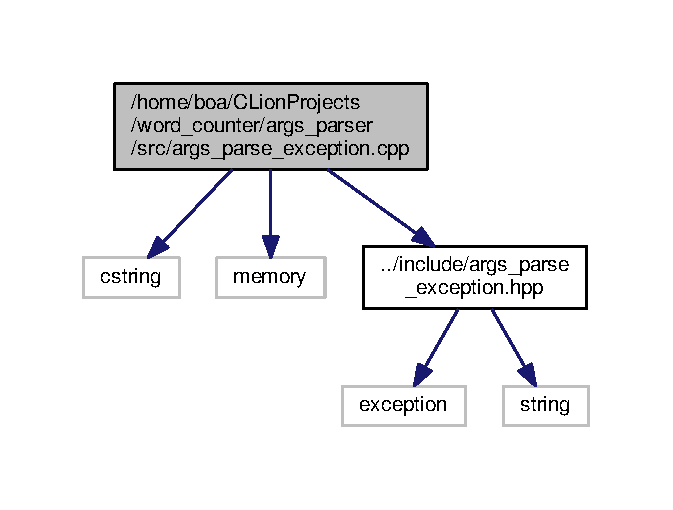
\includegraphics[width=323pt]{args__parse__exception_8cpp__incl}
\end{center}
\end{figure}
\subsection*{Namespaces}
\begin{DoxyCompactItemize}
\item 
 \hyperlink{namespacetwo__gis__test}{two\+\_\+gis\+\_\+test}
\item 
 \hyperlink{namespacetwo__gis__test_1_1argument__parser}{two\+\_\+gis\+\_\+test\+::argument\+\_\+parser}
\end{DoxyCompactItemize}

\hypertarget{argument__parser_8cpp}{}\section{/home/boa/\+C\+Lion\+Projects/word\+\_\+counter/args\+\_\+parser/src/argument\+\_\+parser.cpp File Reference}
\label{argument__parser_8cpp}\index{/home/boa/\+C\+Lion\+Projects/word\+\_\+counter/args\+\_\+parser/src/argument\+\_\+parser.\+cpp@{/home/boa/\+C\+Lion\+Projects/word\+\_\+counter/args\+\_\+parser/src/argument\+\_\+parser.\+cpp}}
{\ttfamily \#include \char`\"{}../include/argument\+\_\+parser.\+hpp\char`\"{}}\\*
{\ttfamily \#include \char`\"{}../include/args\+\_\+parse\+\_\+exception.\+hpp\char`\"{}}\\*
Include dependency graph for argument\+\_\+parser.\+cpp\+:\nopagebreak
\begin{figure}[H]
\begin{center}
\leavevmode
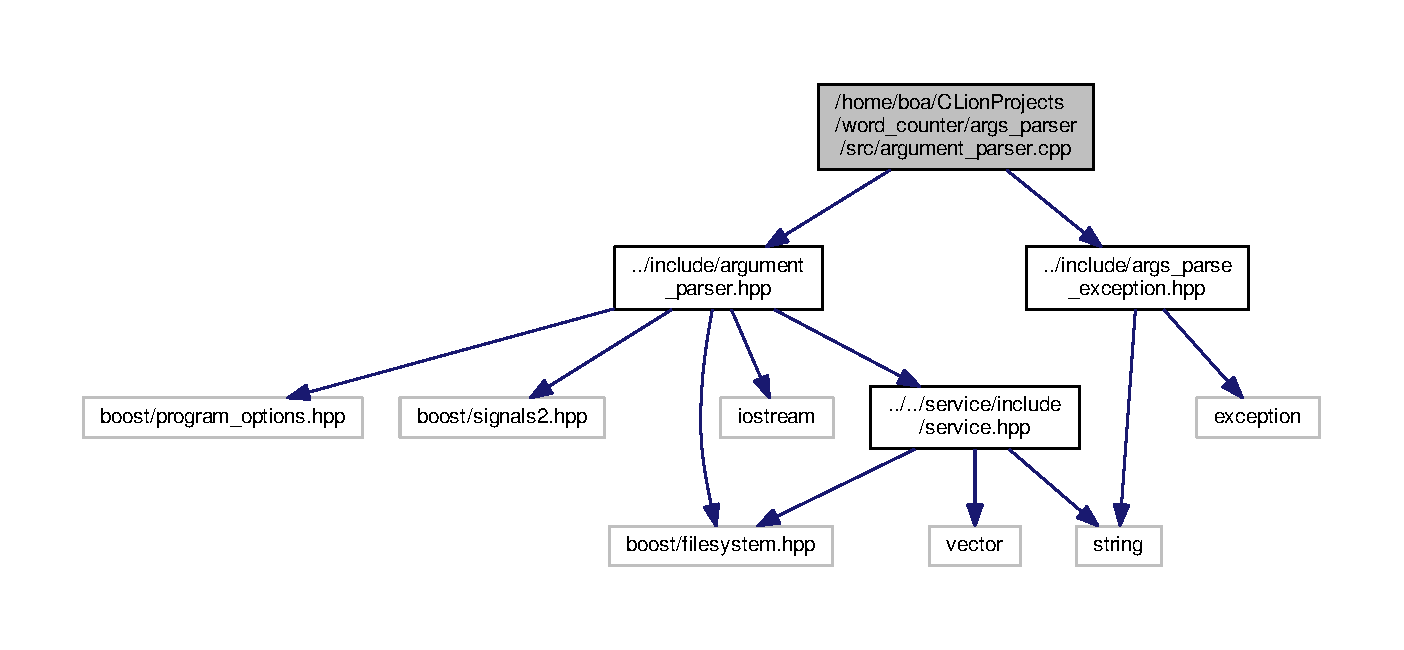
\includegraphics[width=350pt]{argument__parser_8cpp__incl}
\end{center}
\end{figure}
\subsection*{Namespaces}
\begin{DoxyCompactItemize}
\item 
 \hyperlink{namespacetwo__gis__test}{two\+\_\+gis\+\_\+test}
\item 
 \hyperlink{namespacetwo__gis__test_1_1argument__parser}{two\+\_\+gis\+\_\+test\+::argument\+\_\+parser}
\end{DoxyCompactItemize}

\hypertarget{test_8cpp}{}\section{/home/boa/\+C\+Lion\+Projects/word\+\_\+counter/args\+\_\+parser/test/test.cpp File Reference}
\label{test_8cpp}\index{/home/boa/\+C\+Lion\+Projects/word\+\_\+counter/args\+\_\+parser/test/test.\+cpp@{/home/boa/\+C\+Lion\+Projects/word\+\_\+counter/args\+\_\+parser/test/test.\+cpp}}

\hypertarget{checksum__command_8hpp}{}\section{/home/boa/\+C\+Lion\+Projects/word\+\_\+counter/command\+\_\+handler/include/checksum\+\_\+command.hpp File Reference}
\label{checksum__command_8hpp}\index{/home/boa/\+C\+Lion\+Projects/word\+\_\+counter/command\+\_\+handler/include/checksum\+\_\+command.\+hpp@{/home/boa/\+C\+Lion\+Projects/word\+\_\+counter/command\+\_\+handler/include/checksum\+\_\+command.\+hpp}}
{\ttfamily \#include $<$string$>$}\\*
{\ttfamily \#include \char`\"{}icommand.\+hpp\char`\"{}}\\*
Include dependency graph for checksum\+\_\+command.\+hpp\+:\nopagebreak
\begin{figure}[H]
\begin{center}
\leavevmode
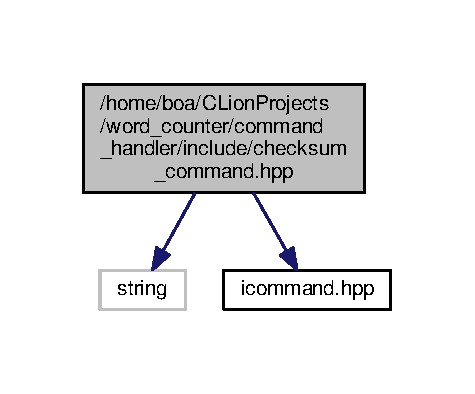
\includegraphics[width=228pt]{checksum__command_8hpp__incl}
\end{center}
\end{figure}
This graph shows which files directly or indirectly include this file\+:\nopagebreak
\begin{figure}[H]
\begin{center}
\leavevmode
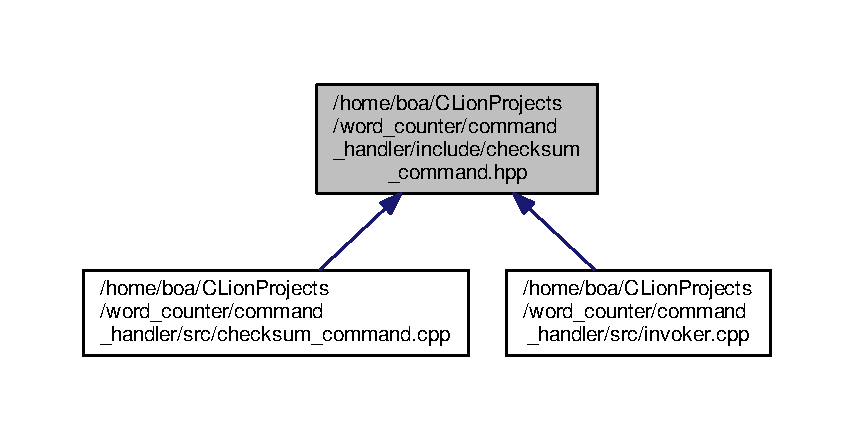
\includegraphics[width=350pt]{checksum__command_8hpp__dep__incl}
\end{center}
\end{figure}
\subsection*{Classes}
\begin{DoxyCompactItemize}
\item 
class \hyperlink{classtwo__gis__test_1_1command__handler_1_1_checksum_command}{two\+\_\+gis\+\_\+test\+::command\+\_\+handler\+::\+Checksum\+Command}
\end{DoxyCompactItemize}
\subsection*{Namespaces}
\begin{DoxyCompactItemize}
\item 
 \hyperlink{namespacetwo__gis__test}{two\+\_\+gis\+\_\+test}
\item 
 \hyperlink{namespacetwo__gis__test_1_1command__handler}{two\+\_\+gis\+\_\+test\+::command\+\_\+handler}
\end{DoxyCompactItemize}

\hypertarget{command__handler_8hpp}{}\section{/home/boa/\+C\+Lion\+Projects/word\+\_\+counter/command\+\_\+handler/include/command\+\_\+handler.hpp File Reference}
\label{command__handler_8hpp}\index{/home/boa/\+C\+Lion\+Projects/word\+\_\+counter/command\+\_\+handler/include/command\+\_\+handler.\+hpp@{/home/boa/\+C\+Lion\+Projects/word\+\_\+counter/command\+\_\+handler/include/command\+\_\+handler.\+hpp}}
{\ttfamily \#include $<$string$>$}\\*
{\ttfamily \#include $<$functional$>$}\\*
{\ttfamily \#include $<$memory$>$}\\*
{\ttfamily \#include \char`\"{}icommand.\+hpp\char`\"{}}\\*
Include dependency graph for command\+\_\+handler.\+hpp\+:\nopagebreak
\begin{figure}[H]
\begin{center}
\leavevmode
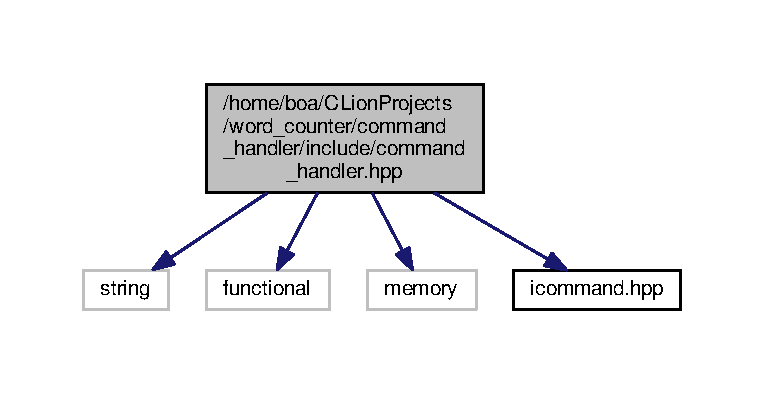
\includegraphics[width=350pt]{command__handler_8hpp__incl}
\end{center}
\end{figure}
This graph shows which files directly or indirectly include this file\+:\nopagebreak
\begin{figure}[H]
\begin{center}
\leavevmode
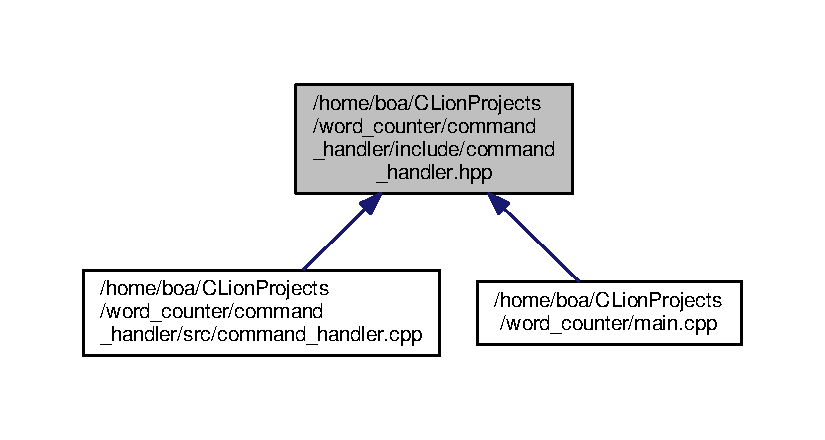
\includegraphics[width=350pt]{command__handler_8hpp__dep__incl}
\end{center}
\end{figure}
\subsection*{Classes}
\begin{DoxyCompactItemize}
\item 
class \hyperlink{classtwo__gis__test_1_1command__handler_1_1_command_handler}{two\+\_\+gis\+\_\+test\+::command\+\_\+handler\+::\+Command\+Handler}
\end{DoxyCompactItemize}
\subsection*{Namespaces}
\begin{DoxyCompactItemize}
\item 
 \hyperlink{namespacetwo__gis__test}{two\+\_\+gis\+\_\+test}
\item 
 \hyperlink{namespacetwo__gis__test_1_1command__handler}{two\+\_\+gis\+\_\+test\+::command\+\_\+handler}
\end{DoxyCompactItemize}

\hypertarget{count__occurrences__word__command_8hpp}{}\section{/home/boa/\+C\+Lion\+Projects/word\+\_\+counter/command\+\_\+handler/include/count\+\_\+occurrences\+\_\+word\+\_\+command.hpp File Reference}
\label{count__occurrences__word__command_8hpp}\index{/home/boa/\+C\+Lion\+Projects/word\+\_\+counter/command\+\_\+handler/include/count\+\_\+occurrences\+\_\+word\+\_\+command.\+hpp@{/home/boa/\+C\+Lion\+Projects/word\+\_\+counter/command\+\_\+handler/include/count\+\_\+occurrences\+\_\+word\+\_\+command.\+hpp}}
{\ttfamily \#include $<$string$>$}\\*
{\ttfamily \#include $<$vector$>$}\\*
{\ttfamily \#include \char`\"{}icommand.\+hpp\char`\"{}}\\*
Include dependency graph for count\+\_\+occurrences\+\_\+word\+\_\+command.\+hpp\+:\nopagebreak
\begin{figure}[H]
\begin{center}
\leavevmode
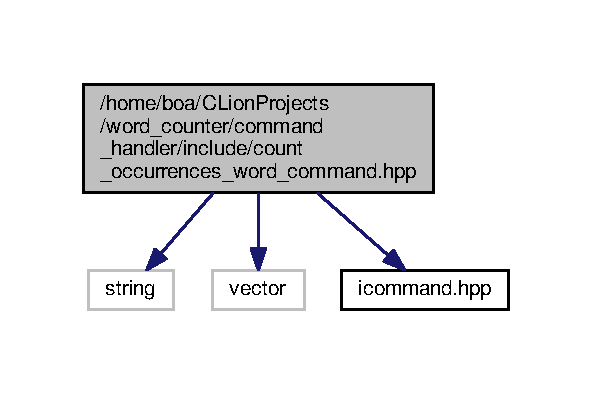
\includegraphics[width=284pt]{count__occurrences__word__command_8hpp__incl}
\end{center}
\end{figure}
This graph shows which files directly or indirectly include this file\+:\nopagebreak
\begin{figure}[H]
\begin{center}
\leavevmode
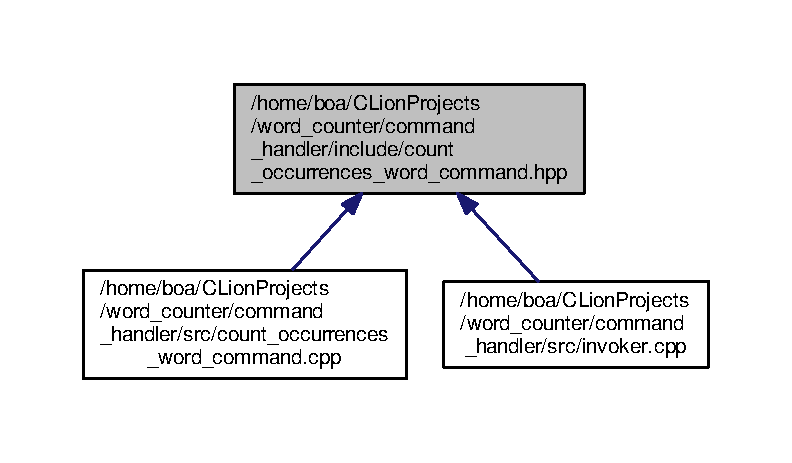
\includegraphics[width=350pt]{count__occurrences__word__command_8hpp__dep__incl}
\end{center}
\end{figure}
\subsection*{Classes}
\begin{DoxyCompactItemize}
\item 
class \hyperlink{classtwo__gis__test_1_1command__handler_1_1_count_occurrences_word_command}{two\+\_\+gis\+\_\+test\+::command\+\_\+handler\+::\+Count\+Occurrences\+Word\+Command}
\end{DoxyCompactItemize}
\subsection*{Namespaces}
\begin{DoxyCompactItemize}
\item 
 \hyperlink{namespacetwo__gis__test}{two\+\_\+gis\+\_\+test}
\item 
 \hyperlink{namespacetwo__gis__test_1_1command__handler}{two\+\_\+gis\+\_\+test\+::command\+\_\+handler}
\end{DoxyCompactItemize}

\hypertarget{icommand_8hpp}{}\section{/home/boa/\+C\+Lion\+Projects/word\+\_\+counter/command\+\_\+handler/include/icommand.hpp File Reference}
\label{icommand_8hpp}\index{/home/boa/\+C\+Lion\+Projects/word\+\_\+counter/command\+\_\+handler/include/icommand.\+hpp@{/home/boa/\+C\+Lion\+Projects/word\+\_\+counter/command\+\_\+handler/include/icommand.\+hpp}}
This graph shows which files directly or indirectly include this file\+:\nopagebreak
\begin{figure}[H]
\begin{center}
\leavevmode
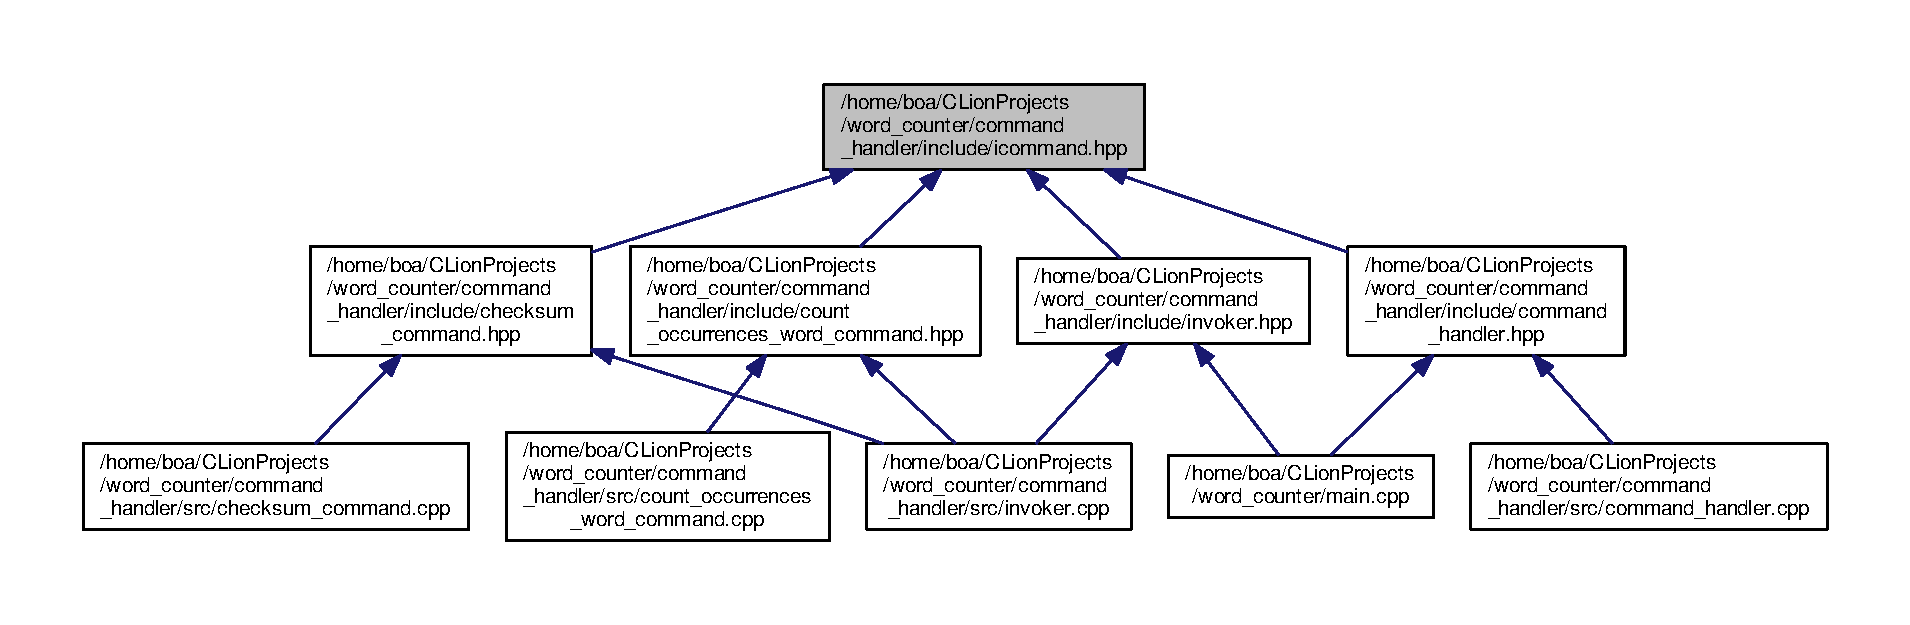
\includegraphics[width=350pt]{icommand_8hpp__dep__incl}
\end{center}
\end{figure}
\subsection*{Classes}
\begin{DoxyCompactItemize}
\item 
class \hyperlink{classtwo__gis__test_1_1command__handler_1_1_i_command}{two\+\_\+gis\+\_\+test\+::command\+\_\+handler\+::\+I\+Command}
\end{DoxyCompactItemize}
\subsection*{Namespaces}
\begin{DoxyCompactItemize}
\item 
 \hyperlink{namespacetwo__gis__test}{two\+\_\+gis\+\_\+test}
\item 
 \hyperlink{namespacetwo__gis__test_1_1command__handler}{two\+\_\+gis\+\_\+test\+::command\+\_\+handler}
\end{DoxyCompactItemize}

\hypertarget{invoker_8hpp}{}\section{/home/boa/\+C\+Lion\+Projects/word\+\_\+counter/command\+\_\+handler/include/invoker.hpp File Reference}
\label{invoker_8hpp}\index{/home/boa/\+C\+Lion\+Projects/word\+\_\+counter/command\+\_\+handler/include/invoker.\+hpp@{/home/boa/\+C\+Lion\+Projects/word\+\_\+counter/command\+\_\+handler/include/invoker.\+hpp}}
{\ttfamily \#include $<$memory$>$}\\*
{\ttfamily \#include $<$boost/signals2.\+hpp$>$}\\*
{\ttfamily \#include \char`\"{}icommand.\+hpp\char`\"{}}\\*
Include dependency graph for invoker.\+hpp\+:\nopagebreak
\begin{figure}[H]
\begin{center}
\leavevmode
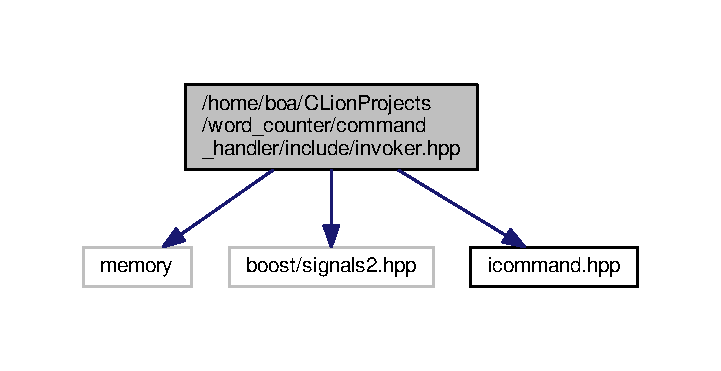
\includegraphics[width=346pt]{invoker_8hpp__incl}
\end{center}
\end{figure}
This graph shows which files directly or indirectly include this file\+:\nopagebreak
\begin{figure}[H]
\begin{center}
\leavevmode
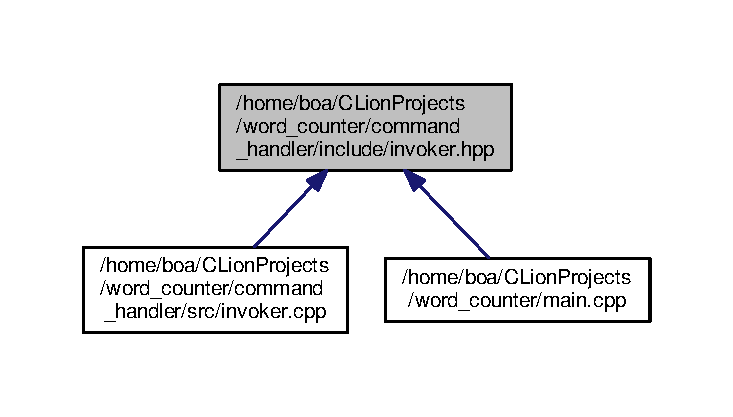
\includegraphics[width=350pt]{invoker_8hpp__dep__incl}
\end{center}
\end{figure}
\subsection*{Classes}
\begin{DoxyCompactItemize}
\item 
class \hyperlink{classtwo__gis__test_1_1command__handler_1_1_invoker}{two\+\_\+gis\+\_\+test\+::command\+\_\+handler\+::\+Invoker}
\end{DoxyCompactItemize}
\subsection*{Namespaces}
\begin{DoxyCompactItemize}
\item 
 \hyperlink{namespacetwo__gis__test}{two\+\_\+gis\+\_\+test}
\item 
 \hyperlink{namespacetwo__gis__test_1_1command__handler}{two\+\_\+gis\+\_\+test\+::command\+\_\+handler}
\end{DoxyCompactItemize}

\hypertarget{checksum__command_8cpp}{}\section{/home/boa/\+C\+Lion\+Projects/word\+\_\+counter/command\+\_\+handler/src/checksum\+\_\+command.cpp File Reference}
\label{checksum__command_8cpp}\index{/home/boa/\+C\+Lion\+Projects/word\+\_\+counter/command\+\_\+handler/src/checksum\+\_\+command.\+cpp@{/home/boa/\+C\+Lion\+Projects/word\+\_\+counter/command\+\_\+handler/src/checksum\+\_\+command.\+cpp}}
{\ttfamily \#include $<$iostream$>$}\\*
{\ttfamily \#include $<$fstream$>$}\\*
{\ttfamily \#include \char`\"{}../include/checksum\+\_\+command.\+hpp\char`\"{}}\\*
{\ttfamily \#include \char`\"{}../../service/include/service.\+hpp\char`\"{}}\\*
Include dependency graph for checksum\+\_\+command.\+cpp\+:\nopagebreak
\begin{figure}[H]
\begin{center}
\leavevmode
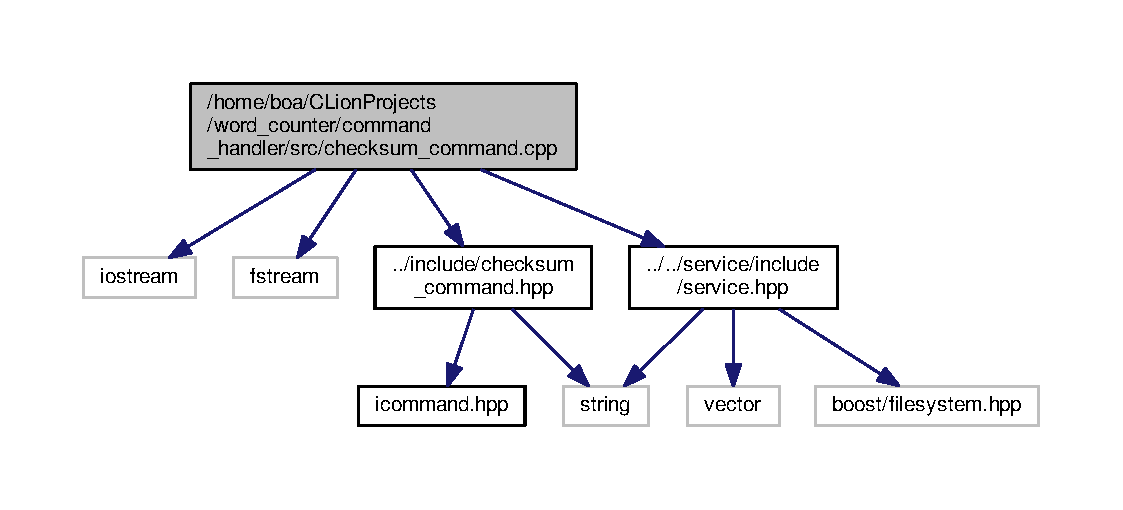
\includegraphics[width=350pt]{checksum__command_8cpp__incl}
\end{center}
\end{figure}
\subsection*{Namespaces}
\begin{DoxyCompactItemize}
\item 
 \hyperlink{namespacetwo__gis__test}{two\+\_\+gis\+\_\+test}
\item 
 \hyperlink{namespacetwo__gis__test_1_1command__handler}{two\+\_\+gis\+\_\+test\+::command\+\_\+handler}
\end{DoxyCompactItemize}

\hypertarget{command__handler_8cpp}{}\section{/home/boa/\+C\+Lion\+Projects/word\+\_\+counter/command\+\_\+handler/src/command\+\_\+handler.cpp File Reference}
\label{command__handler_8cpp}\index{/home/boa/\+C\+Lion\+Projects/word\+\_\+counter/command\+\_\+handler/src/command\+\_\+handler.\+cpp@{/home/boa/\+C\+Lion\+Projects/word\+\_\+counter/command\+\_\+handler/src/command\+\_\+handler.\+cpp}}
{\ttfamily \#include \char`\"{}../include/command\+\_\+handler.\+hpp\char`\"{}}\\*
Include dependency graph for command\+\_\+handler.\+cpp\+:\nopagebreak
\begin{figure}[H]
\begin{center}
\leavevmode
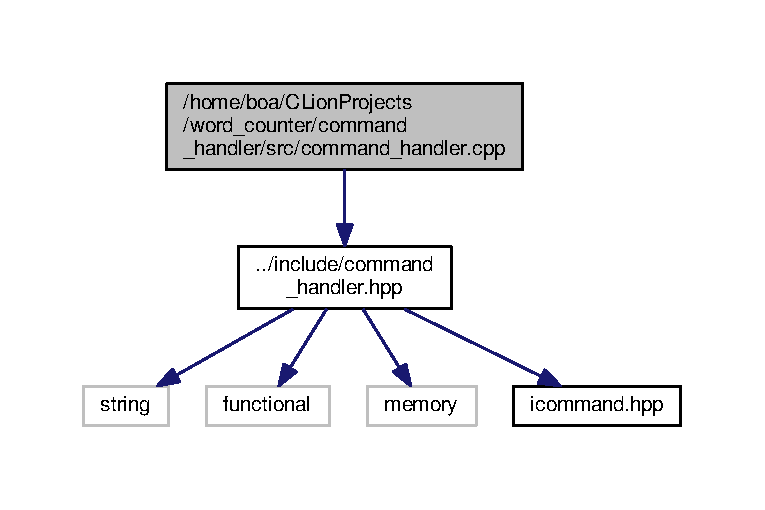
\includegraphics[width=350pt]{command__handler_8cpp__incl}
\end{center}
\end{figure}
\subsection*{Namespaces}
\begin{DoxyCompactItemize}
\item 
 \hyperlink{namespacetwo__gis__test}{two\+\_\+gis\+\_\+test}
\item 
 \hyperlink{namespacetwo__gis__test_1_1command__handler}{two\+\_\+gis\+\_\+test\+::command\+\_\+handler}
\end{DoxyCompactItemize}

\hypertarget{count__occurrences__word__command_8cpp}{}\section{/home/boa/\+C\+Lion\+Projects/word\+\_\+counter/command\+\_\+handler/src/count\+\_\+occurrences\+\_\+word\+\_\+command.cpp File Reference}
\label{count__occurrences__word__command_8cpp}\index{/home/boa/\+C\+Lion\+Projects/word\+\_\+counter/command\+\_\+handler/src/count\+\_\+occurrences\+\_\+word\+\_\+command.\+cpp@{/home/boa/\+C\+Lion\+Projects/word\+\_\+counter/command\+\_\+handler/src/count\+\_\+occurrences\+\_\+word\+\_\+command.\+cpp}}
{\ttfamily \#include $<$iostream$>$}\\*
{\ttfamily \#include $<$fstream$>$}\\*
{\ttfamily \#include $<$boost/system/error\+\_\+code.\+hpp$>$}\\*
{\ttfamily \#include \char`\"{}../include/count\+\_\+occurrences\+\_\+word\+\_\+command.\+hpp\char`\"{}}\\*
{\ttfamily \#include \char`\"{}../../service/include/service.\+hpp\char`\"{}}\\*
Include dependency graph for count\+\_\+occurrences\+\_\+word\+\_\+command.\+cpp\+:\nopagebreak
\begin{figure}[H]
\begin{center}
\leavevmode
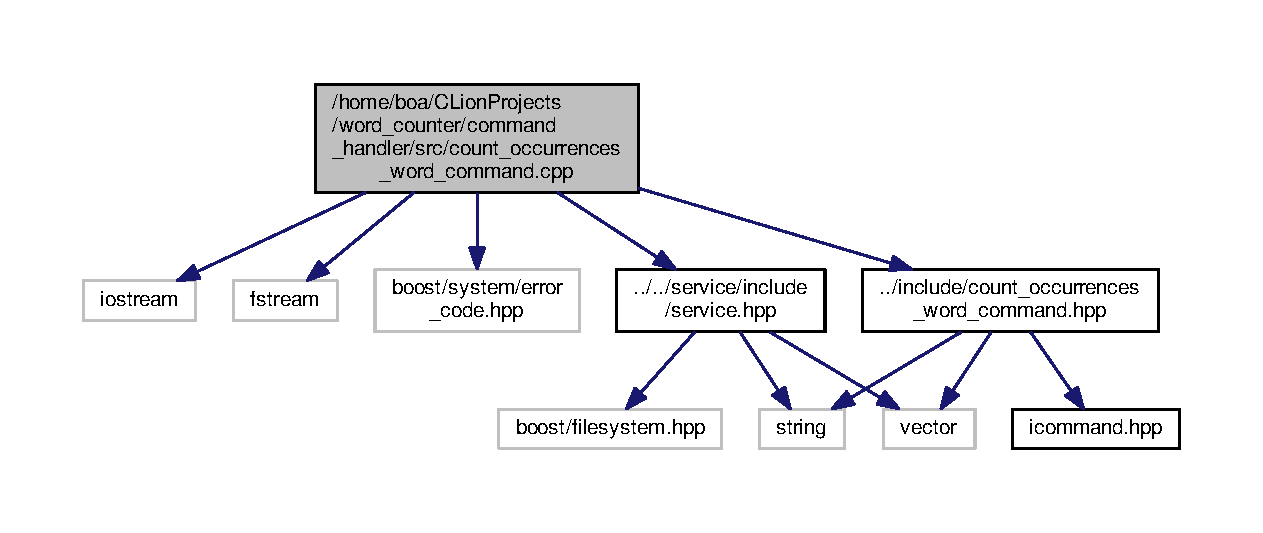
\includegraphics[width=350pt]{count__occurrences__word__command_8cpp__incl}
\end{center}
\end{figure}
\subsection*{Namespaces}
\begin{DoxyCompactItemize}
\item 
 \hyperlink{namespacetwo__gis__test}{two\+\_\+gis\+\_\+test}
\item 
 \hyperlink{namespacetwo__gis__test_1_1command__handler}{two\+\_\+gis\+\_\+test\+::command\+\_\+handler}
\end{DoxyCompactItemize}

\hypertarget{invoker_8cpp}{}\section{/home/boa/\+C\+Lion\+Projects/word\+\_\+counter/command\+\_\+handler/src/invoker.cpp File Reference}
\label{invoker_8cpp}\index{/home/boa/\+C\+Lion\+Projects/word\+\_\+counter/command\+\_\+handler/src/invoker.\+cpp@{/home/boa/\+C\+Lion\+Projects/word\+\_\+counter/command\+\_\+handler/src/invoker.\+cpp}}
{\ttfamily \#include \char`\"{}../include/invoker.\+hpp\char`\"{}}\\*
{\ttfamily \#include \char`\"{}../include/count\+\_\+occurrences\+\_\+word\+\_\+command.\+hpp\char`\"{}}\\*
{\ttfamily \#include \char`\"{}../include/checksum\+\_\+command.\+hpp\char`\"{}}\\*
Include dependency graph for invoker.\+cpp\+:\nopagebreak
\begin{figure}[H]
\begin{center}
\leavevmode
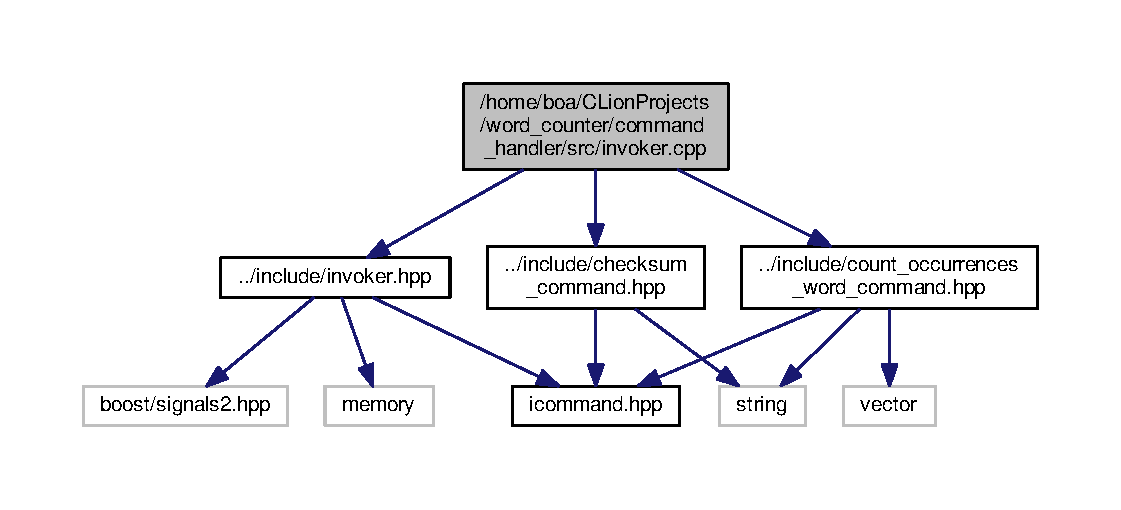
\includegraphics[width=350pt]{invoker_8cpp__incl}
\end{center}
\end{figure}
\subsection*{Namespaces}
\begin{DoxyCompactItemize}
\item 
 \hyperlink{namespacetwo__gis__test}{two\+\_\+gis\+\_\+test}
\item 
 \hyperlink{namespacetwo__gis__test_1_1command__handler}{two\+\_\+gis\+\_\+test\+::command\+\_\+handler}
\end{DoxyCompactItemize}

\hypertarget{main_8cpp}{}\section{/home/boa/\+C\+Lion\+Projects/word\+\_\+counter/main.cpp File Reference}
\label{main_8cpp}\index{/home/boa/\+C\+Lion\+Projects/word\+\_\+counter/main.\+cpp@{/home/boa/\+C\+Lion\+Projects/word\+\_\+counter/main.\+cpp}}
{\ttfamily \#include $<$iostream$>$}\\*
{\ttfamily \#include \char`\"{}args\+\_\+parser/include/argument\+\_\+parser.\+hpp\char`\"{}}\\*
{\ttfamily \#include \char`\"{}command\+\_\+handler/include/command\+\_\+handler.\+hpp\char`\"{}}\\*
{\ttfamily \#include \char`\"{}args\+\_\+parser/include/args\+\_\+parse\+\_\+exception.\+hpp\char`\"{}}\\*
{\ttfamily \#include \char`\"{}command\+\_\+handler/include/invoker.\+hpp\char`\"{}}\\*
Include dependency graph for main.\+cpp\+:\nopagebreak
\begin{figure}[H]
\begin{center}
\leavevmode
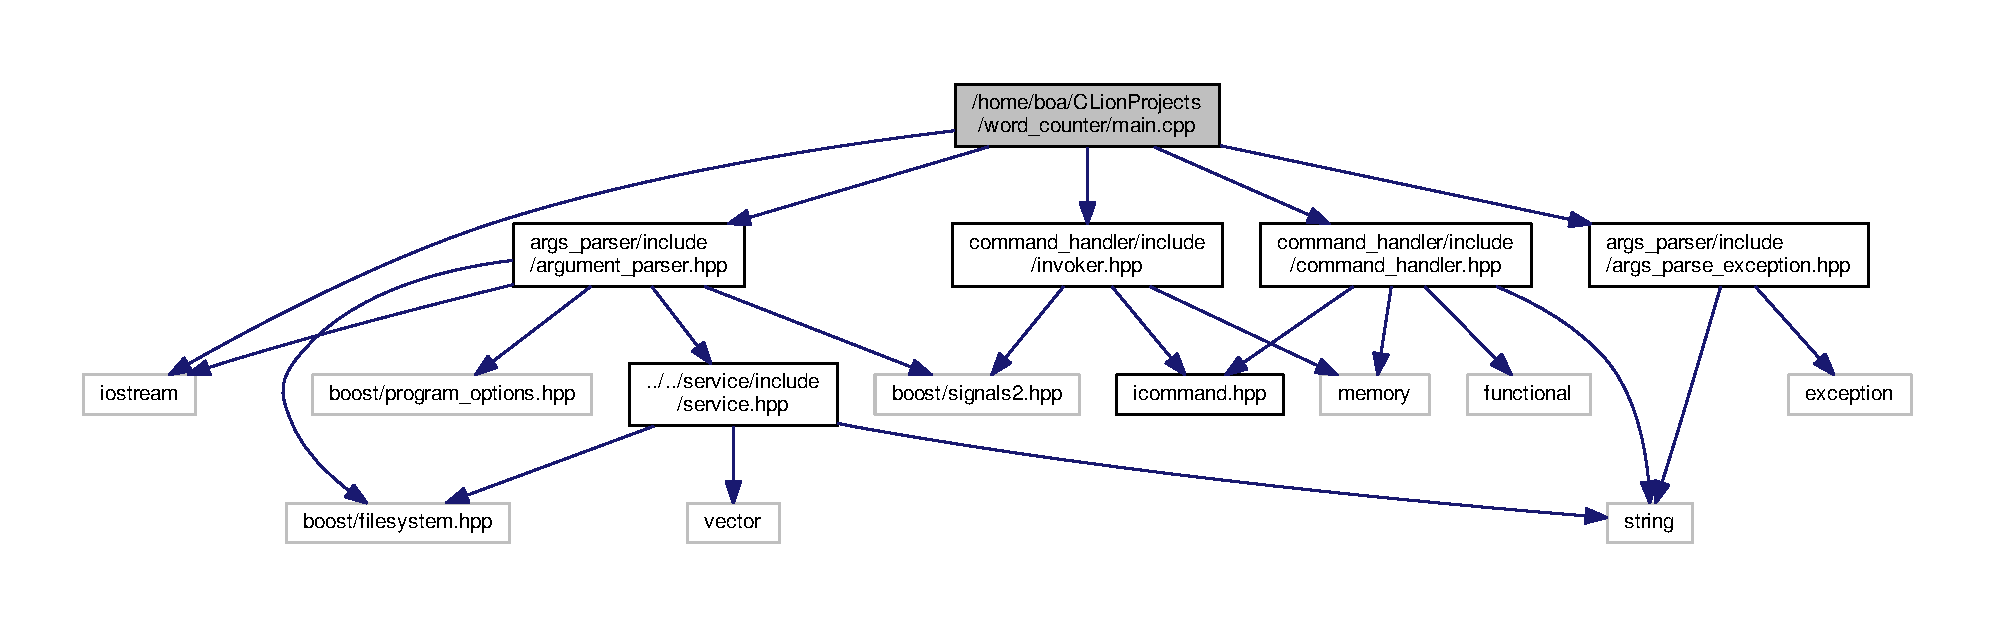
\includegraphics[width=350pt]{main_8cpp__incl}
\end{center}
\end{figure}
\subsection*{Functions}
\begin{DoxyCompactItemize}
\item 
int \hyperlink{main_8cpp_a0ddf1224851353fc92bfbff6f499fa97}{main} (int argc, char $\ast$argv\mbox{[}$\,$\mbox{]})
\end{DoxyCompactItemize}


\subsection{Function Documentation}
\index{main.\+cpp@{main.\+cpp}!main@{main}}
\index{main@{main}!main.\+cpp@{main.\+cpp}}
\subsubsection[{\texorpdfstring{main(int argc, char $\ast$argv[])}{main(int argc, char *argv[])}}]{\setlength{\rightskip}{0pt plus 5cm}int main (
\begin{DoxyParamCaption}
\item[{int}]{argc, }
\item[{char $\ast$}]{argv\mbox{[}$\,$\mbox{]}}
\end{DoxyParamCaption}
)}\hypertarget{main_8cpp_a0ddf1224851353fc92bfbff6f499fa97}{}\label{main_8cpp_a0ddf1224851353fc92bfbff6f499fa97}


Definition at line 22 of file main.\+cpp.



Here is the call graph for this function\+:\nopagebreak
\begin{figure}[H]
\begin{center}
\leavevmode
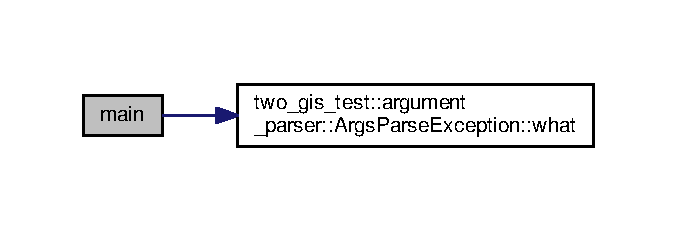
\includegraphics[width=325pt]{main_8cpp_a0ddf1224851353fc92bfbff6f499fa97_cgraph}
\end{center}
\end{figure}



\hypertarget{service_8hpp}{}\section{/home/boa/\+C\+Lion\+Projects/word\+\_\+counter/service/include/service.hpp File Reference}
\label{service_8hpp}\index{/home/boa/\+C\+Lion\+Projects/word\+\_\+counter/service/include/service.\+hpp@{/home/boa/\+C\+Lion\+Projects/word\+\_\+counter/service/include/service.\+hpp}}
{\ttfamily \#include $<$vector$>$}\\*
{\ttfamily \#include $<$string$>$}\\*
{\ttfamily \#include $<$boost/filesystem.\+hpp$>$}\\*
Include dependency graph for service.\+hpp\+:\nopagebreak
\begin{figure}[H]
\begin{center}
\leavevmode
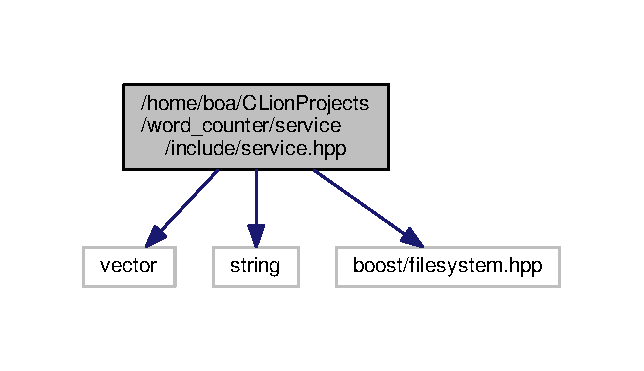
\includegraphics[width=309pt]{service_8hpp__incl}
\end{center}
\end{figure}
This graph shows which files directly or indirectly include this file\+:\nopagebreak
\begin{figure}[H]
\begin{center}
\leavevmode
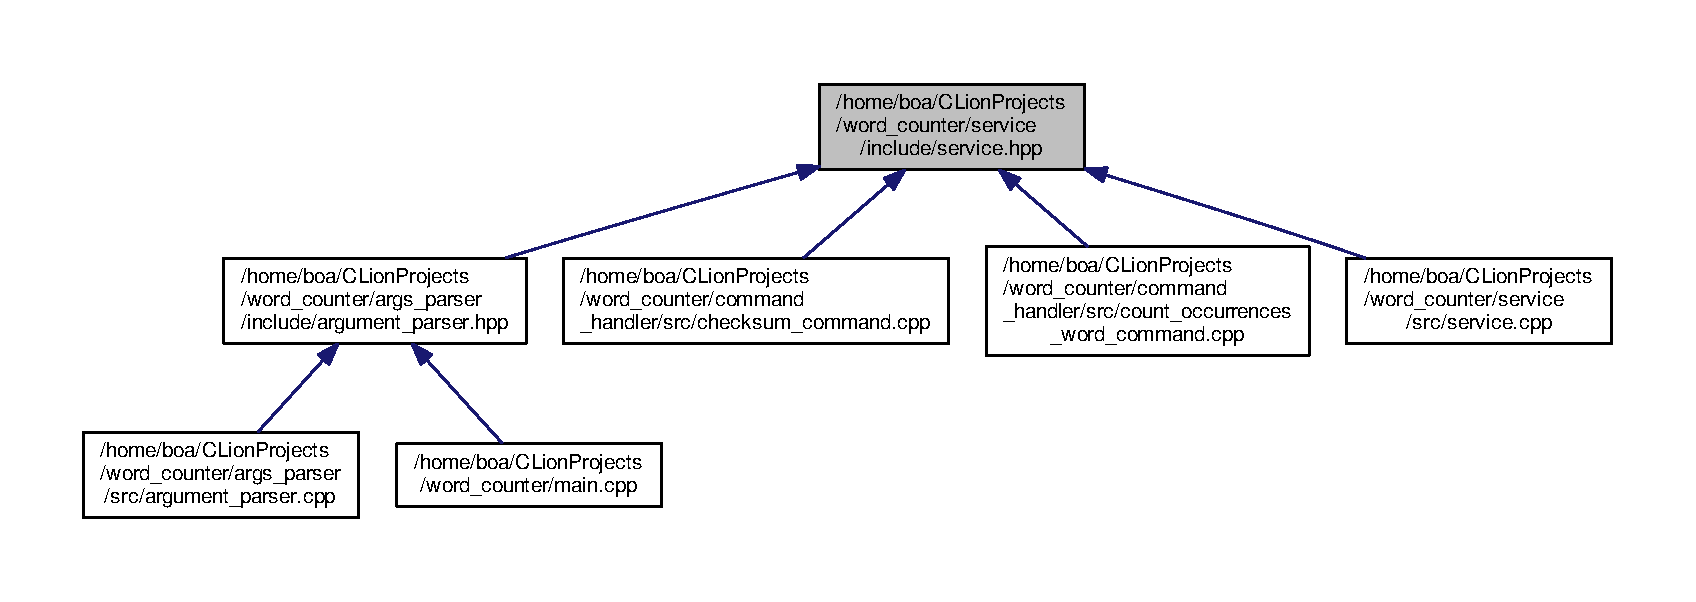
\includegraphics[width=350pt]{service_8hpp__dep__incl}
\end{center}
\end{figure}
\subsection*{Namespaces}
\begin{DoxyCompactItemize}
\item 
 \hyperlink{namespacetwo__gis__test}{two\+\_\+gis\+\_\+test}
\item 
 \hyperlink{namespacetwo__gis__test_1_1service}{two\+\_\+gis\+\_\+test\+::service}
\end{DoxyCompactItemize}
\subsection*{Functions}
\begin{DoxyCompactItemize}
\item 
bool \hyperlink{namespacetwo__gis__test_1_1service_ae373eed74cdbd1fd23749a7cd25ec61f}{two\+\_\+gis\+\_\+test\+::service\+::is\+Valid\+File} (const std\+::string \&filename, boost\+::system\+::error\+\_\+code \&error\+Code)
\begin{DoxyCompactList}\small\item\em is\+Valid\+File -\/ checks the existence of the file and its status \end{DoxyCompactList}\end{DoxyCompactItemize}

\hypertarget{service_8cpp}{}\section{/home/boa/\+C\+Lion\+Projects/word\+\_\+counter/service/src/service.cpp File Reference}
\label{service_8cpp}\index{/home/boa/\+C\+Lion\+Projects/word\+\_\+counter/service/src/service.\+cpp@{/home/boa/\+C\+Lion\+Projects/word\+\_\+counter/service/src/service.\+cpp}}
{\ttfamily \#include \char`\"{}../include/service.\+hpp\char`\"{}}\\*
Include dependency graph for service.\+cpp\+:\nopagebreak
\begin{figure}[H]
\begin{center}
\leavevmode
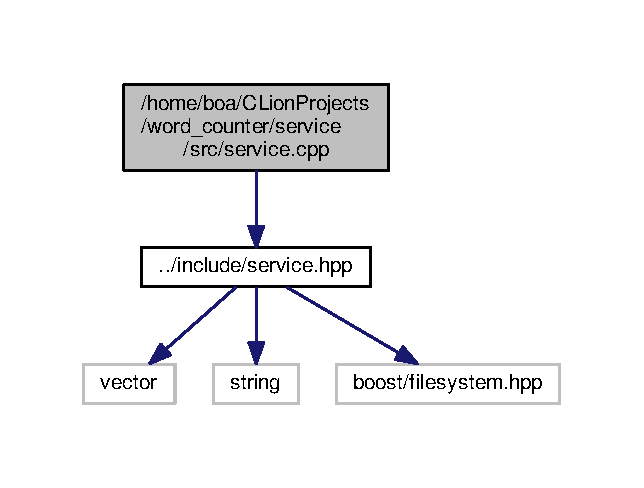
\includegraphics[width=309pt]{service_8cpp__incl}
\end{center}
\end{figure}
\subsection*{Namespaces}
\begin{DoxyCompactItemize}
\item 
 \hyperlink{namespacetwo__gis__test}{two\+\_\+gis\+\_\+test}
\item 
 \hyperlink{namespacetwo__gis__test_1_1service}{two\+\_\+gis\+\_\+test\+::service}
\end{DoxyCompactItemize}
\subsection*{Functions}
\begin{DoxyCompactItemize}
\item 
bool \hyperlink{namespacetwo__gis__test_1_1service_ae373eed74cdbd1fd23749a7cd25ec61f}{two\+\_\+gis\+\_\+test\+::service\+::is\+Valid\+File} (const std\+::string \&filename, boost\+::system\+::error\+\_\+code \&error\+Code)
\begin{DoxyCompactList}\small\item\em is\+Valid\+File -\/ checks the existence of the file and its status \end{DoxyCompactList}\end{DoxyCompactItemize}

%--- End generated contents ---

% Index
\backmatter
\newpage
\phantomsection
\clearemptydoublepage
\addcontentsline{toc}{chapter}{Index}
\printindex

\end{document}
